\documentclass[a4paper,12pt]{book}
%  A simple AAU report template.
%  2015-05-08 v. 1.2.0
%  Copyright 2010-2015 by Jesper Kjær Nielsen <jkn@es.aau.dk>
%
%  This is free software: you can redistribute it and/or modify
%  it under the terms of the GNU General Public License as published by
%  the Free Software Foundation, either version 3 of the License, or
%  (at your option) any later version.
%
%  This is distributed in the hope that it will be useful,
%  but WITHOUT ANY WARRANTY; without even the implied warranty of
%  MERCHANTABILITY or FITNESS FOR A PARTICULAR PURPOSE.  See the
%  GNU General Public License for more details.
%
%  You can find the GNU General Public License at <http://www.gnu.org/licenses/>.
%
%%%%%%%%%%%%%%%%%%%%%%%%%%%%%%%%%%%%%%%%%%%%%%%%
% Language, Encoding and Fonts
% http://en.wikibooks.org/wiki/LaTeX/Internationalization
%%%%%%%%%%%%%%%%%%%%%%%%%%%%%%%%%%%%%%%%%%%%%%%%
% Select encoding of your inputs. Depends on
% your operating system and its default input
% encoding. Typically, you should use
%   Linux  : utf8 (most modern Linux distributions)
%            latin1 
%   Windows: ansinew
%            latin1 (works in most cases)
%   Mac    : applemac
% Notice that you can manually change the input
% encoding of your files by selecting "save as"
% an select the desired input encoding. 
\usepackage[utf8]{inputenc}
% Make latex understand and use the typographic
% rules of the language used in the document.
\usepackage[english]{babel}
% Use the palatino font
\usepackage[sc]{mathpazo}
\usepackage{gensymb}
\linespread{1.1}         % Palatino needs more leading (space between lines)
% Choose the font encoding
\usepackage[T1]{fontenc}
%%%%%%%%%%%%%%%%%%%%%%%%%%%%%%%%%%%%%%%%%%%%%%%%
% Graphics and Tables
% http://en.wikibooks.org/wiki/LaTeX/Importing_Graphics
% http://en.wikibooks.org/wiki/LaTeX/Tables
% http://en.wikibooks.org/wiki/LaTeX/Colors
%%%%%%%%%%%%%%%%%%%%%%%%%%%%%%%%%%%%%%%%%%%%%%%%
% load a colour package
\usepackage{xcolor}
\definecolor{aaublue}{RGB}{33,26,82}% dark blue
% The standard graphics inclusion package
\usepackage{graphicx}
% Set up how figure and table captions are displayed
\usepackage{caption}
\captionsetup{%
  font=footnotesize,% set font size to footnotesize
  labelfont=bf % bold label (e.g., Figure 3.2) font
}
% Make the standard latex tables look so much better
\usepackage{array,booktabs}
% Enable the use of frames around, e.g., theorems
% The framed package is used in the example environment
\usepackage{framed}
\usepackage{wrapfig}
%%%%%%%%%%%%%%%%%%%%%%%%%%%%%%%%%%%%%%%%%%%%%%%%
% Mathematics
% http://en.wikibooks.org/wiki/LaTeX/Mathematics
%%%%%%%%%%%%%%%%%%%%%%%%%%%%%%%%%%%%%%%%%%%%%%%%
% Defines new environments such as equation,
% align and split 
\usepackage{amsmath}
% Adds new math symbols
\usepackage{amssymb}
% Use theorems in your document
% The ntheorem package is also used for the example environment
% When using thmmarks, amsmath must be an option as well. Otherwise \eqref doesn't work anymore.
\usepackage[framed,amsmath,thmmarks]{ntheorem}
\usepackage{pdfpages}
%%%%%%%%%%%%%%%%%%%%%%%%%%%%%%%%%%%%%%%%%%%%%%%%
% Page Layout
% http://en.wikibooks.org/wiki/LaTeX/Page_Layout
%%%%%%%%%%%%%%%%%%%%%%%%%%%%%%%%%%%%%%%%%%%%%%%%
% Change margins, papersize, etc of the document
\usepackage[
  a4paper,
  top=28mm,
  inner=20mm,% left margin on an odd page
  outer=20mm,% right margin on an odd page
  bottom=20mm
  ]{geometry}
% Modify how \chapter, \section, etc. look
% The titlesec package is very configureable
%\usepackage{titlesec}
%\titleformat{\chapter}[display]{\normalfont\huge\bfseries}{\chaptertitlename\ \thechapter}{20pt}{\Huge}
%\titleformat*{\section}{\normalfont\Large\bfseries}
%\titleformat*{\subsection}{\normalfont\large\bfseries}
%\titleformat*{\subsubsection}{\normalfont\normalsize\bfseries}
%\titleformat*{\paragraph}{\normalfont\normalsize\bfseries}
%\titleformat*{\subparagraph}{\normalfont\normalsize\bfseries}

% Clear empty pages between chapters
\let\origdoublepage\cleardoublepage
\newcommand{\clearemptydoublepage}{%
  \clearpage
  {\pagestyle{empty}\origdoublepage}%
}
\let\cleardoublepage\clearemptydoublepage

% Change the headers and footers
\usepackage{fancyhdr}
\pagestyle{fancy}
\fancyhf{} %delete everything
\renewcommand{\headrulewidth}{1pt} %remove the horizontal line in the header
\fancyhead[RE]{\small\nouppercase\leftmark} %even page - chapter title
\fancyhead[LO]{\small\nouppercase\rightmark} %uneven page - section title
\fancyhead[LE,RO]{\thepage} %page number on all pages
% Do not stretch the content of a page. Instead,
% insert white space at the bottom of the page
\raggedbottom
% Enable arithmetics with length. Useful when
% typesetting the layout.
\usepackage{calc}
\usepackage{svg}
\addto\captionsenglish{% Replace "english" with the language you use
  \renewcommand{\contentsname}%
    {Table of contents}%
}

%%%%%%%%%%%%%%%%%%%%%%%%%%%%%%%%%%%%%%%%%%%%%%%%
% Misc
%%%%%%%%%%%%%%%%%%%%%%%%%%%%%%%%%%%%%%%%%%%%%%%%
% Add bibliography and index to the table of
% contents
\usepackage[nottoc]{tocbibind}
% Add the command \pageref{LastPage} which refers to the
% page number of the last page
\usepackage{lastpage}
% Add todo notes in the margin of the document
\usepackage[
%  disable, %turn off todonotes
  colorinlistoftodos, %enable a coloured square in the list of todos
  textwidth=\marginparwidth, %set the width of the todonotes
  textsize=scriptsize, %size of the text in the todonotes
  ]{todonotes}

%%%%%%%%%%%%%%%%%%%%%%%%%%%%%%%%%%%%%%%%%%%%%%%%
% Hyperlinks
% http://en.wikibooks.org/wiki/LaTeX/Hyperlinks
%%%%%%%%%%%%%%%%%%%%%%%%%%%%%%%%%%%%%%%%%%%%%%%%
% Enable hyperlinks and insert info into the pdf
% file. Hypperref should be loaded as one of the 
% last packages
\usepackage{hyperref}
\hypersetup{%
	pdfpagelabels=true,%
	plainpages=false,%
	pdfauthor={Author(s)},%
	pdftitle={Title},%
	pdfsubject={Subject},%
	bookmarksnumbered=true,%
	colorlinks=false,%
	citecolor=black,%
	filecolor=black,%
	linkcolor=black,% you should probably change this to black before printing
	urlcolor=black,%
	pdfstartview=FitH%
}


\usepackage{amsmath}
\usepackage{amssymb}
%  A simple AAU report template.
%  2015-05-08 v. 1.2.0
%  Copyright 2010-2015 by Jesper Kjær Nielsen <jkn@es.aau.dk>
%
%  This is free software: you can redistribute it and/or modify
%  it under the terms of the GNU General Public License as published by
%  the Free Software Foundation, either version 3 of the License, or
%  (at your option) any later version.
%
%  This is distributed in the hope that it will be useful,
%  but WITHOUT ANY WARRANTY; without even the implied warranty of
%  MERCHANTABILITY or FITNESS FOR A PARTICULAR PURPOSE.  See the
%  GNU General Public License for more details.
%
%  You can find the GNU General Public License at <http://www.gnu.org/licenses/>.
%
%
%
% see, e.g., http://en.wikibooks.org/wiki/LaTeX/Customizing_LaTeX#New_commands
% for more information on how to create macros

%%%%%%%%%%%%%%%%%%%%%%%%%%%%%%%%%%%%%%%%%%%%%%%%
% Macros for the titlepage
%%%%%%%%%%%%%%%%%%%%%%%%%%%%%%%%%%%%%%%%%%%%%%%%
%Creates the aau titlepage
\newcommand{\aautitlepage}[3]{%
  {
    %set up various length
    \ifx\titlepageleftcolumnwidth\undefined
      \newlength{\titlepageleftcolumnwidth}
      \newlength{\titlepagerightcolumnwidth}
    \fi
    \setlength{\titlepageleftcolumnwidth}{0.5\textwidth-\tabcolsep}
    \setlength{\titlepagerightcolumnwidth}{\textwidth-2\tabcolsep-\titlepageleftcolumnwidth}
    %create title page
    \thispagestyle{empty}
    \noindent%
    \begin{tabular}{@{}ll@{}}
      \parbox{\titlepageleftcolumnwidth}{
        \iflanguage{danish}{%
          \includegraphics[width=\titlepageleftcolumnwidth]{figures/aau_logo_da}
        }{%
          
\includegraphics[width=\titlepageleftcolumnwidth]{Figures/aau_logo_en.pdf}
        }
      } &
      \parbox{\titlepagerightcolumnwidth}{\raggedleft\sf\small
        #2
      }\bigskip\\
       #1 &
      \parbox[t]{\titlepagerightcolumnwidth}{%
      \textbf{Abstract:}\bigskip\par
        \fbox{\parbox{\titlepagerightcolumnwidth-2\fboxsep-2\fboxrule}{%
          #3
        }}
      }\\
    \end{tabular}
    \vfill
    \iflanguage{danish}{%
      \noindent{\footnotesize\emph{Rapportens indhold er frit tilgængeligt, men offentliggørelse (med kildeangivelse) må kun ske efter aftale med forfatterne.}}
    }{%
      \noindent{\footnotesize\emph{The content of this report is freely available, but publication (with reference) may only be pursued due to agreement with the author.}}
    }
    \clearpage
  }
}

%Create english project info
\newcommand{\englishprojectinfo}[8]{%
  \parbox[t]{\titlepageleftcolumnwidth}{
    \textbf{Title:}\\ #1\bigskip\par
    \textbf{Theme:}\\ #2\bigskip\par
    \textbf{Project Period:}\\ #3\bigskip\par
    \textbf{Project Group:}\\ #4\bigskip\par
    \textbf{Participants:}\\ #5\bigskip\par
    \textbf{Supervisor:}\\ #6\bigskip\par
    \textbf{Copies:} #7\bigskip\par
    \textbf{Page Numbers:} \pageref{LastPage}\bigskip\par
    \textbf{Date of Completion:}\\ #8
  }
}

%Create danish project info
\newcommand{\danishprojectinfo}[8]{%
  \parbox[t]{\titlepageleftcolumnwidth}{
    \textbf{Titel:}\\ #1\bigskip\par
    \textbf{Tema:}\\ #2\bigskip\par
    \textbf{Projektperiode:}\\ #3\bigskip\par
    \textbf{Projektgruppe:}\\ #4\bigskip\par
    \textbf{Deltager(e):}\\ #5\bigskip\par
    \textbf{Vejleder(e):}\\ #6\bigskip\par
    \textbf{Oplagstal:} #7\bigskip\par
    \textbf{Sidetal:} \pageref{LastPage}\bigskip\par
    \textbf{Afleveringsdato:}\\ #8
  }
}

\makeatletter
\newsavebox\myboxA
\newsavebox\myboxB
\newlength\mylenA

\newcommand*{\rom}[1]{\expandafter\@slowromancap\romannumeral #1@}

\newcommand*\xoverline[2][0.75]{%
    \sbox{\myboxA}{$\m@th#2$}%
    \setbox\myboxB\null% Phantom box
    \ht\myboxB=\ht\myboxA%
    \dp\myboxB=\dp\myboxA%
    \wd\myboxB=#1\wd\myboxA% Scale phantom
    \sbox\myboxB{$\m@th\overline{\copy\myboxB}$}%  Overlined phantom
    \setlength\mylenA{\the\wd\myboxA}%   calc width diff
    \addtolength\mylenA{-\the\wd\myboxB}%
    \ifdim\wd\myboxB<\wd\myboxA%
       \rlap{\hskip 0.5\mylenA\usebox\myboxB}{\usebox\myboxA}%
    \else
        \hskip -0.5\mylenA\rlap{\usebox\myboxA}{\hskip 0.5\mylenA\usebox\myboxB}%
    \fi}
\makeatother

%%%%%%%%%%%%%%%%%%%%%%%%%%%%%%%%%%%%%%%%%%%%%%%%
% An example environment
%%%%%%%%%%%%%%%%%%%%%%%%%%%%%%%%%%%%%%%%%%%%%%%%
\theoremheaderfont{\normalfont\bfseries}
\theorembodyfont{\normalfont}
\theoremstyle{break}
\def\theoremframecommand{{\color{gray!50}\vrule width 5pt \hspace{5pt}}}
\newshadedtheorem{exa}{Example}[chapter]
\newenvironment{example}[1]{%
		\begin{exa}[#1]
}{%
		\end{exa}
}

\usepackage{array}
\usepackage{siunitx} % adds SI units
\usepackage{placeins} % includes FloatBarrier
\usepackage{graphicx}
\usepackage{epstopdf}
\usepackage{caption}
\usepackage{subcaption}
\usepackage{amsmath}
\usepackage{amsfonts}
\usepackage{mathtools}
\usepackage{float}
\usepackage{gensymb}
\usepackage{csvsimple}
\usepackage{hhline}
\usepackage{pdfpages}
\usepackage[T1]{fontenc}
\usepackage{stix} 
\usepackage{gensymb}
\usepackage{listings}
\usepackage{color} %red, green, blue, yellow, cyan, magenta, black, white
\definecolor{mygreen}{RGB}{28,172,0} % color values Red, Green, Blue
\definecolor{mylilas}{RGB}{170,55,241}

\usepackage[backend=biber, sorting=none]{biblatex}
\usepackage{booktabs}
\addbibresource{articles.bib}
%\renewcommand{\thesection}{\hspace*{-1.0em}}
%\renewcommand{\thesection}{\arabic{section}}

\newcommand{\argmin}{\operatornamewithlimits{argmin}}
\newcommand{\argmax}{\operatornamewithlimits{argmax}}

\lstset{language=Matlab,%
    %basicstyle=\color{red},
    breaklines=true,%
    morekeywords={matlab2tikz},
    keywordstyle=\color{blue},%
    morekeywords=[2]{1}, keywordstyle=[2]{\color{black}},
    identifierstyle=\color{black},%
    stringstyle=\color{mylilas},
    commentstyle=\color{mygreen},%
    showstringspaces=false,%without this there will be a symbol in the places where there is a space
    numbers=left,%
    numberstyle={\tiny \color{black}},% size of the numbers
    numbersep=9pt, % this defines how far the numbers are from the text
    emph=[1]{for,end,break},emphstyle=[1]\color{red}, %some words to emphasise
    %emph=[2]{word1,word2}, emphstyle=[2]{style},    
}

\usepackage{etoolbox}
%\usepackage{tocloft}
%\usepackage[titles]{tocloft}
%\usepackage[bottom]{footmisc}
\usepackage[titletoc]{appendix}
\setcounter{secnumdepth}{2}
\setcounter{tocdepth}{2}

%\begin{titlepage}
%	\rule{1pt}{1.1\textheight} % Vertical line
%	\hspace{0.02\textwidth} 
%	\parbox[b]{0.95\textwidth}{ \\
%		
%		{\huge \bfseries Report\\[\baselineskip]}
%		{\large SDM vs Binaural:\\ A comparison of different room auralization techniques}\\[2\baselineskip]
%		{\large\textit{Acoustics and Audio Technology }\\{9th semester project}}\\
%		{\large Aalborg University\\[4\baselineskip]}
%		
%		\vspace{0.6\textheight}
%		{\noindent Ashwin~~~~~~~~~~~~~~~~~~~~~~~~~~~~~~~~~~~~~~~~~~ Maxime}\\[0\baselineskip]
%		{\noindent Saraf~~~~~~~~~~~~~~~~~~~~~~~~~~~~~~~~~~~~~~~~~~~ Démurger}}
%
%\end{titlepage} 


\usepackage[intoc]{nomencl}
\usepackage{amsmath}
\usepackage{amssymb}
\usepackage{pgfplots}
\usepackage{mathtools}

\pgfplotsset{compat=1.9}


\usepackage[bottom]{footmisc}

\begin{document}

\begin{figure}[H]
    \centering
    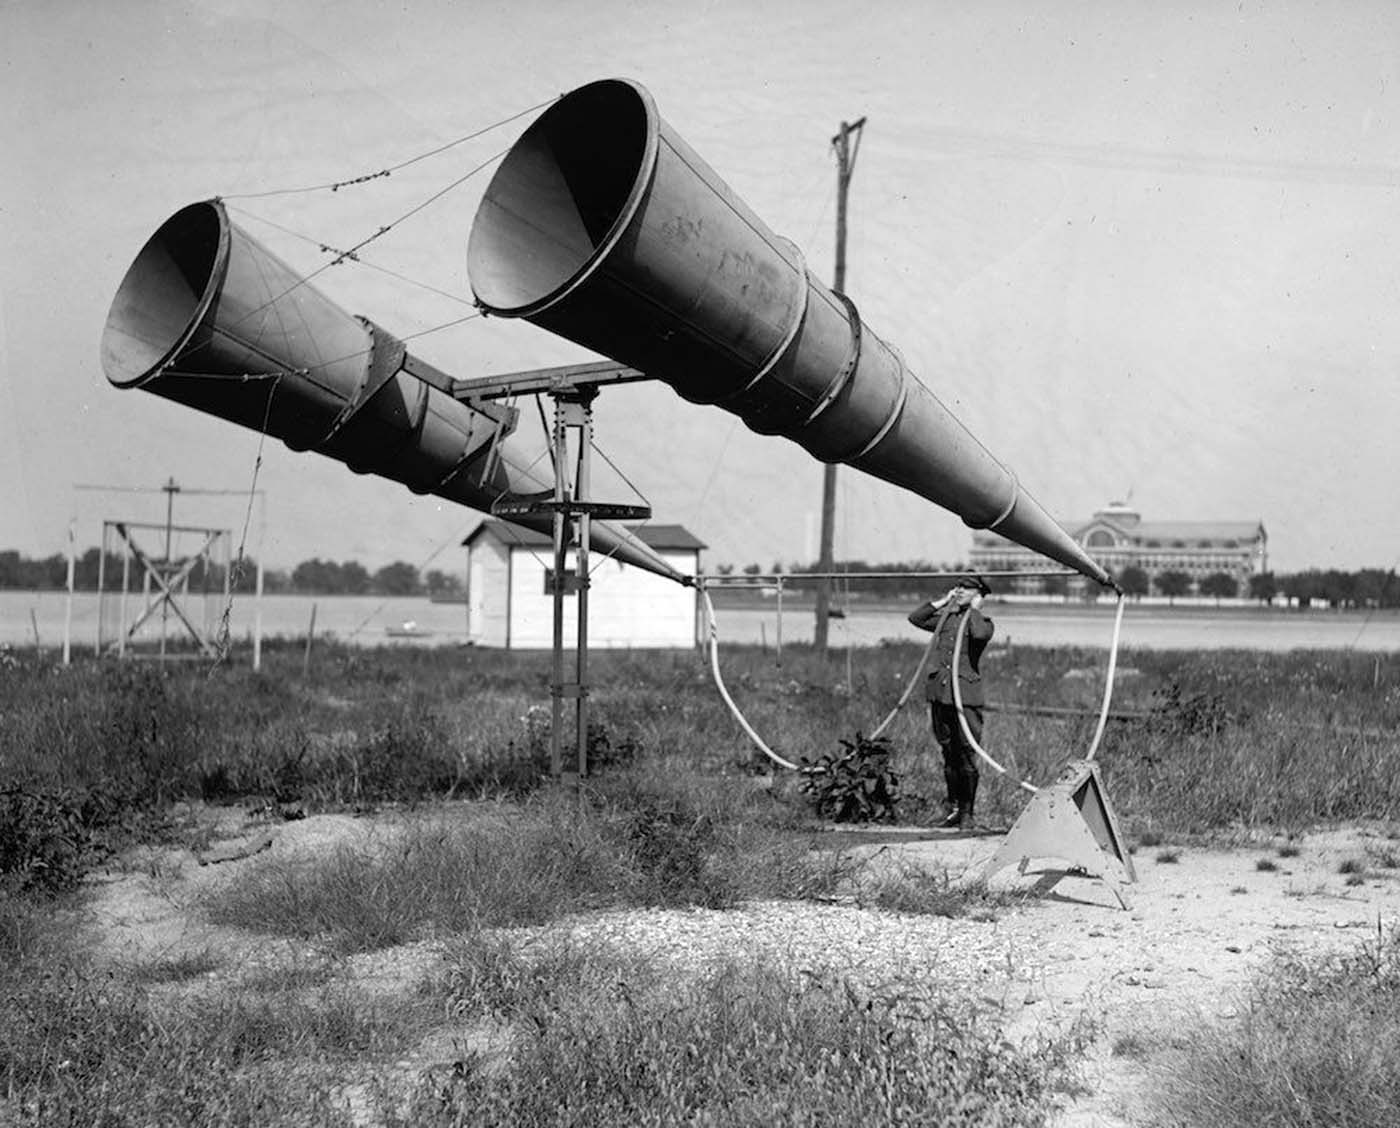
\includegraphics[width=1\textwidth]{Figures/acousticloc.jpg}
    \label{fig:acousticloc}
\end{figure}

\thispagestyle{empty}
{\small
\strut\vfill % push the content to the bottom of the page
\noindent Copyright \copyright{} Aalborg University 2018\par
\vspace{0.2cm}
\noindent This report has been compiled using \LaTeX.
}
\clearpage

\newpage
\pdfbookmark[0]{English title page}{label:titlepage_en}
\aautitlepage{%
  \englishprojectinfo{
    Outdoor Sound Localization using a tetrahedral microphone array %title
  }{%
    Master's Thesis %theme
  }{%
    Fall Semester 2018 %project period
  }{%
    AAT10-1062 % project group
  }{%
    %list of group members
    Ashwin Saraf\\ 
    Maxime Démurger
  }{%
    %list of supervisors
    Søren Krarup Olesen\\
  }{%
    1 % number of printed copies
  }{%
    \today % date of completion
  }%
}{%department and address
  \textbf{Electronics and IT}\\
  Aalborg University\\
  \href{http://www.aau.dk}{http://www.aau.dk}
}{% the abstract
   The impact of sound on individual's health can be dramatic when one is exposed to high sound pressure level (SPL) for a long period of time. While SPL at concerts are measurable using one microphone, it can be difficult to do the same in outdoor environments when multiple sources are present. This work aims at developing a monitoring system to localize the main outdoor noise contributors while retrieving their SPL. Using signal processing and a microphone array to capture the sound, it is possible to compute a sound map of the array surroundings. Sound localization techniques have been implemented successfully in a wide range of product, notably the SRP-PHAT algorithm which combines the beamforming techniques and time difference of arrival (TDOA) information. However this method is designed for sources in a reverberant field while the outdoor environment is sensibly different. This works improves the robustness of SRP-PHAT for outdoor sound localization and present a method to deconvolve the array response from the result. This new algorithm, the MP-SRP-PHAT is presented and experimentally evaluated in various conditions. The algorithm improves SRP-PHAT when multiple sources are present on the map however it cannot handle coherent sources.
  
}


\frontmatter
\section*{Preface}\\

\vspace{1cm}

This report has been carried out during Spring of 2018 as a Acoustics and Audio Technology Master's Thesis at Aalborg University by group 10GR1062.\\

\noindent
The group would like to thank Søren Krarup Olesen (Associate Professor, AAU) and Karim Haddad (Research engineer, Brüel \& Kjær)  for their supervision throughout the project.\\

\noindent
The figures in the report are produced by the group unless a source is specified.\\

\noindent

\newcommand{\doubleSignature}[5]{
\begin{minipage}[c]{\textwidth}
\vspace{2cm}

\makebox[12cm][c]{
 #1, \today 
}
\vspace{3cm}

\makebox[12cm][c]{
\hfill \makebox[5cm][c] {\hrulefill} \hfill \makebox[5cm][c] {\hrulefill} \hfill
}
\makebox[12cm][c]{
\hfill #2 \hfill #3 \hfill
}
\makebox[12cm][c]{
\hfill #4 \hfill #5 \hfill
}
\vspace{1cm}
\end{minipage}
}

\doubleSignature{Aalborg}{Ashwin Saraf}{Maxime Démurger}{asaraf16@student.aau.dk}{mdemur16@student.aau.dk}


\tableofcontents


\makenomenclature
\renewcommand{\nomname}{Glossary of terms}

\nomenclature{\textbf{MP-SRP-PHAT}}{Minimum Power Steered Response Power PHAT}
\nomenclature{\textbf{Array aperture}}{Distance between two microphones in a uniform microphone array}


\printnomenclature
\mainmatter
\chapter{Introduction}

\section{Motivation}
Sound has been a subject of fascination for a long time and with good reason. We have known since prehistoric times that sound travels slower than light, evermore proven whenever a flash of lightning was seen before the clap was heard \cite{ampel1993history}.  In 1636AD, Marin Mersènne of Paris used a pendulum to make speed of sound measurements by firing cannons. The $\rom{19}^{th}$ century mark the first attempts to create transducers and Graham Bell invention of the phone in 1876 mark a clear step forward in the technology allowing to transmit intelligible sounds. While the transducer technology was slowly developing, the inability to process the data limited the development of sound localization tool. The beginnings of sound localization can be trace back during the $\rom{20}^{th}$ century war, when rudimentary systems were developed to localize incoming enemy airplanes, giant rotating waveguides were used by an operator to steer and amplify the sound arriving from a given direction, the prequel of beamforming. For a long time, ears were the only tool to localize sound, until the development of computer and array signal processing techniques. Sound localization technology has matured since then and is now part of our daily life and implemented in countless products such as hearing aid, headset, etc.. making our life much easier in the end. This technology can now be used to solve new problems such as accessing the impact of environmental noise on human. This impact is still been studied by researchers around the world \footnote{some study claim that sound can cause health issue. Regulation are still being written to quantify a safe daily noise exposure} and a reliable noise monitoring system is yet to be developed to detect the main noise contributors in an outdoor environment. This thesis tackle the problem of localizing and quantifying main noise disturbance in outdoor environment. The main challenges of sound localization arise in developing a robust technique to localize multiple sources in a changing complex outdoor sound field. This thesis propose a method to solve this problem.

\section{Background}

Sound localization algorithms have been successfully applied (to varying degrees) to a wide range of engineering problems. Traditionally, distinction is usually made between algorithm using the time difference of arrival (TDOA) \nomenclature{\textbf{TDOA}}{Time Difference Of Arrival}  of signal between pairs microphones to find the position of a source and the algorithm using beamforming Steered Response Power (SRP). However, the SRP-PHAT algorithm, one of the most robust and widely implemented technique combines the advantages of those two techniques. A significant bit of research has been done on implementing SRP-PHAT on speech enhancement systems, whereby speaker identification and teleconferencing in an environment having high background noise and reverberant conditions was needed. Outdoor sound can be appreciably different from this situation. This thesis proposes a method to adapt the SRP-PHAT to compute a sound map of a multi-source outdoor environment.

\begin{figure}[H]
    \centering
    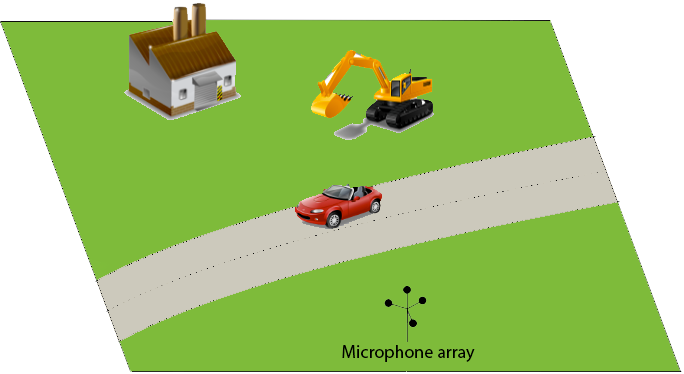
\includegraphics[width=0.8\textwidth]{Figures/scenariofarfield.png}
    \caption{Various outdoor sound sources being localized by a microphone array}
    \label{fig:Introductioncase}
\end{figure}

\section{Scope and outline of the thesis}

This thesis focus mainly on source signal spectrum ranging from low-to-mid frequencies in the far field. It should be noted that the purpose of this thesis is not to track moving sources, rather the thesis tackles the problem of \textit{static outdoor sound levels and their contributors} with the constraint of using as few microphones as possible while being robust to different noise and weather conditions. The thesis propose a solution capable of retrieving the noise source position in a variety of scenario including free-field to moderate reverberating environments. While previous research mostly tackle the problem of single source localization using linear or circular arrays, this thesis use a tetrahedral array to capture the signals.

The organization of the thesis is as follows: Chapter 2 derives the theory used to analyze the problem and create our simulation framework. Chapter 3 focus on describing the methods employed to solve the problem as well as algorithm features and its robustness and performance in outdoor conditions the algorithm performance.
Chapter 4 contains experimental results, anechoic and outdoor measurements investigating the algorithm limits in a variety of scenario.
Chapter 5 encompass a discussion about the solution and propose new ideas and further work.





%\section{Tetrahedral microphone array}
A unit vector $\overline{u}$ in 3d space can be defined in spherical coordinates by (1,$\theta$,$\phi$), where the magnitude of the vector is 1, $\theta$ the azimuth and $\phi$ the elevation [3d space point fig here]. We get
\begin{equation}
    \begin{split}
        x_u&=cos(\theta)cos(\phi) \\
        y_u&=sin(\theta)cos(\phi) \\
        z_u&=sin(\phi),
    \end{split}
\end{equation}
this can be denoted by the unit propagation vector ${a(\theta,\phi)}$ in the Cartesian coordinates
\begin{equation}
    a(\theta,\phi)=\begin{bmatrix}cos(\theta)cos(\phi) \\sin(\theta)cos(\phi) \\sin(\phi)\end{bmatrix},
\end{equation}
Suppose sound is travelling along the unit vector $\overline{u}$. Let 2 microphones be placed at positions $\overline{p_1}=(x_1,y_1,z_1)$ and $\overline{p_2}=(x_2,y_2,z_2)$.  Then $\overline{p_{12}}=\overline{p_{2}}-\overline{p_{1}}$, where ${\overline{p_{12}}}$ is the distance between the two microphones. The projection of this distance in the direction of $\overline{u}$ is simply $a(\theta,\phi)\overline{p_{12}}$ and the time it takes for sound to travel between the two microphones is then 
\begin{equation}
    T_{12}=\frac{a(\theta,\phi)\overline{p_{12}}}{c},
\end{equation} c being the speed of sound. For 4 microphones, a Least-Squares approach could be considered, with $^4C_2$ combinations possible. The 'correct' DOA is then the $a(\Theta,\Phi)$ which minimizes the cost function
\begin{equation}
    J(\Theta,\Phi) = \sum\bigg(T_{ij}-\frac{a(\Theta,\Phi)\overline{p_{ij}}}{c}\bigg)^2, \text{for } i,j \in \begin{pmatrix}4\\2\end{pmatrix}.
\end{equation}

Using atleast 4 microphones a spatial array can be constructed. The simplest spatial structure with 4 vertices is a tetrahedron (a triangular pyramid). The tetrahedron has 4 vertices, 4 faces and 6 edges. If the tetrahedron is regular then all the vertices are equally spaced from each other and every face is an equilateral triangle.The following section discusses the simulated performance of different TDOA and DOA algorithms on a tetrahedral array in an outdoor environment.

\subsection{Regular tetrahedral array}

%Let's define a regular tetrahedral array geometry as follows
%\begin{equation}
%    \begin{split}
%        p_1 &= \begin{bmatrix}{-0.5} & {0} & {0}\end{bmatrix}^T \\
%        p_2 &= \begin{bmatrix}{0.5} & {0} & {0}\end{bmatrix}^T \\
%        p_3 &= \begin{bmatrix}{0} & {\sqrt{(0.75)}} & {0}\end{bmatrix}^T \\
%        p_4 &= \begin{bmatrix}{0} & {\sqrt{(0.75)/2}} & {\sqrt{(0.5)}}\end{bmatrix}^T,
%    \end{split}
%\end{equation}


\begin{figure}[H]
    \centering
    \begin{subfigure}[b]{0.48\textwidth}
    \centering
    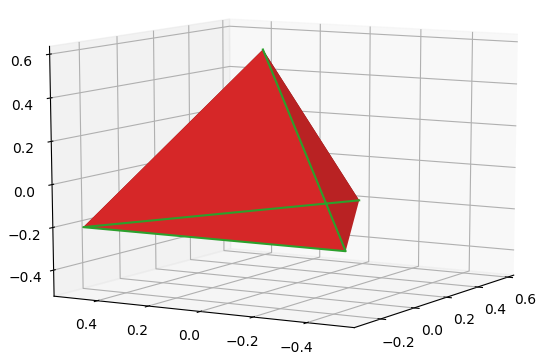
\includegraphics[width=0.9\textwidth]{Figures/unit_tetra.png}
    \caption{Frontal view}
    \label{fig:d1}
\end{subfigure}
\hfill
\begin{subfigure}[b]{0.48\textwidth}
    \centering
    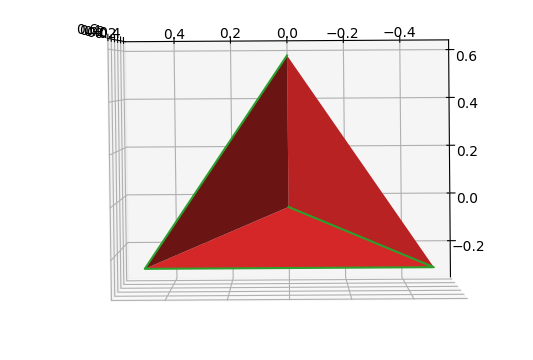
\includegraphics[width=0.9\textwidth]{Figures/unit_tetra_top.png}
    \caption{Top view}
    \label{fig:d2}
\end{subfigure}
    \caption{Representation of a regular Tetrahedral with unit side, centroid at origin and horizontally level lower face, front view and top view}
    \label{fig:regulartetra}
\end{figure}

The distance between the microphones (array aperture) for the tetrahedron in Fig. \ref{fig:regulartetra} is 1m. For such an array, spatial aliasing would occur for frequencies $> (c*1m)/2 \approx $170Hz, c being the speed on sound.  When Fourier based techniques are used for non-stationary signal, the spatial frequency must satisfy the Nyquist Frequency (i.e be $< c/2$) but this requirement can be relaxed for a stationary signal by using anti-aliasing techniques \cite{dmochowski2009spatial}. Fig. \ref{fig:directivityregulartetra} shows the directivity of a tetrahedral array for various frequencies. As expected, aliasing occurs and the main lobe disappears for frequencies $> c/2$. Fig. \ref{fig:directivityothers} shows the directivity for a 4-element uniform linear array (ULA) and uniform circular array (UCA) with the same array aperture of 1m. Since no elevation information can be retrieved from a uni-dimensional linear array the directivity pattern is donut shaped, meaning that the source is located somewhere on the donut. 


\begin{figure}[H]
\centering
\begin{subfigure}{.5\textwidth}
    \centering
        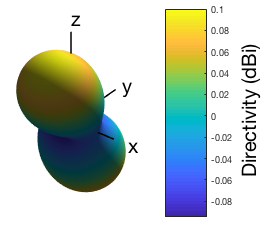
\includegraphics[width=0.7\textwidth]{Figures/regulartetra50hzdirectivity.png}
    \label{fig:directivity200hzregulartetra}
\end{subfigure}%
\begin{subfigure}{.5\textwidth}
        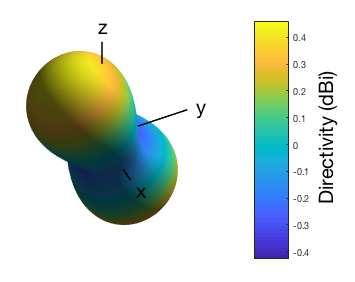
\includegraphics[width=0.7\textwidth]{Figures/regulartetra100hzdirectivity.png}
    \label{fig:directivity100hzregulartetra}
\end{subfigure}
\begin{subfigure}{.5\textwidth}
    \centering
        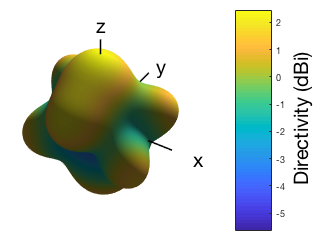
\includegraphics[width=0.9\textwidth]{Figures/regulartetra200hzdirectivity.png}
    \label{fig:directivity200hzregulartetra}
\end{subfigure}%
\begin{subfigure}{.5\textwidth}
    \centering
        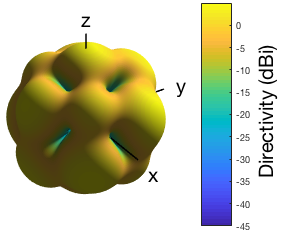
\includegraphics[width=0.9\textwidth]{Figures/regulartetra400hz.png}
    \label{fig:directivity400hzregulartetra}
\end{subfigure}
\caption{Directivity of the regular tetrahedral array at 50hz (top), 100hz(right), 200hz (bottom left) and 400hz (bottom right)}
\label{fig:directivityregulartetra}
\end{figure}


\begin{figure}[H]
\centering
\begin{subfigure}{.5\textwidth}
    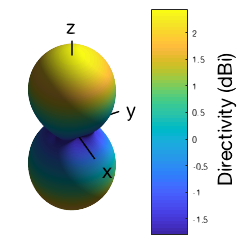
\includegraphics[width=0.85\textwidth]{Figures/uca100hzdirectivity4mic.png}
    \label{fig:directivity100hzuca}
\end{subfigure}%
\begin{subfigure}{.5\textwidth}
    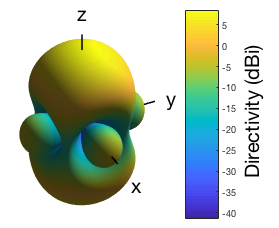
\includegraphics[width=0.85\textwidth]{Figures/uca200hzdirectivity4mic.png}
    \label{fig:directivity100hzuca}
\end{subfigure}%
\caption{Directivity of the UCA array at 100hz(left) and 200hz (right)}
%\label{fig:test}
\end{figure}

\begin{figure}[H]
\centering
\begin{subfigure}{.5\textwidth}
    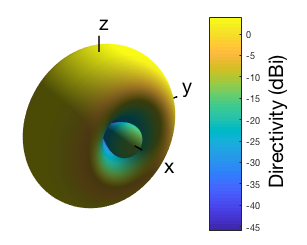
\includegraphics[width=0.85\textwidth]{Figures/ula100hzdirectivity.png}
    \label{fig:directivity100hzuca}
\end{subfigure}%
\begin{subfigure}{.5\textwidth}
    \centering
    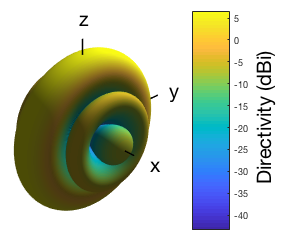
\includegraphics[width=1.1\textwidth]{Figures/ula200hzdirectivity.png}
    \label{fig:directivity100hzula}
\end{subfigure}
\caption{Directivity of the ULA array at 100hz (left) and 200hz (right)}
\label{fig:directivityothers}
\end{figure}
\section{Direction of arrival using time delay information}
\subsection{Time delay between a single microphone pair}\label{sec:TDOA}

When using a pair of microphones, sound from a particular source arrives at the two microphones at different times, based on the source distance to the particular microphone. For a pair of microphones located at $m_{1}$ and $m_{2}$, the time difference of arrival (TDOA) of a sound signal from a source located at s can be defined as:
\begin{equation}
    \begin{split}
    T(\{m_{1},m_{2}\},s)&=\frac{|s-m_{1}|-|s-m_{2}|}{c}\\
                        &=\frac{|D_{1}|-|D_{2}|}{c}
    \label{eq:tdoa}
    \end{split}
\end{equation}
where c is the speed of sound in the medium and $|D_{1}|$ and $|D_{2}|$ the distance between the source and the microphones at $m_1$ and $m_2$.

In 2D, this equation leads to a hyperbola (Fig.\ref{eq:tdoa}) where the two focus points of the hyperbola are the sensors. The difference of the distance from any point of the hyperbola to the two focus is always the same.

\begin{figure}[H]
    \centering
    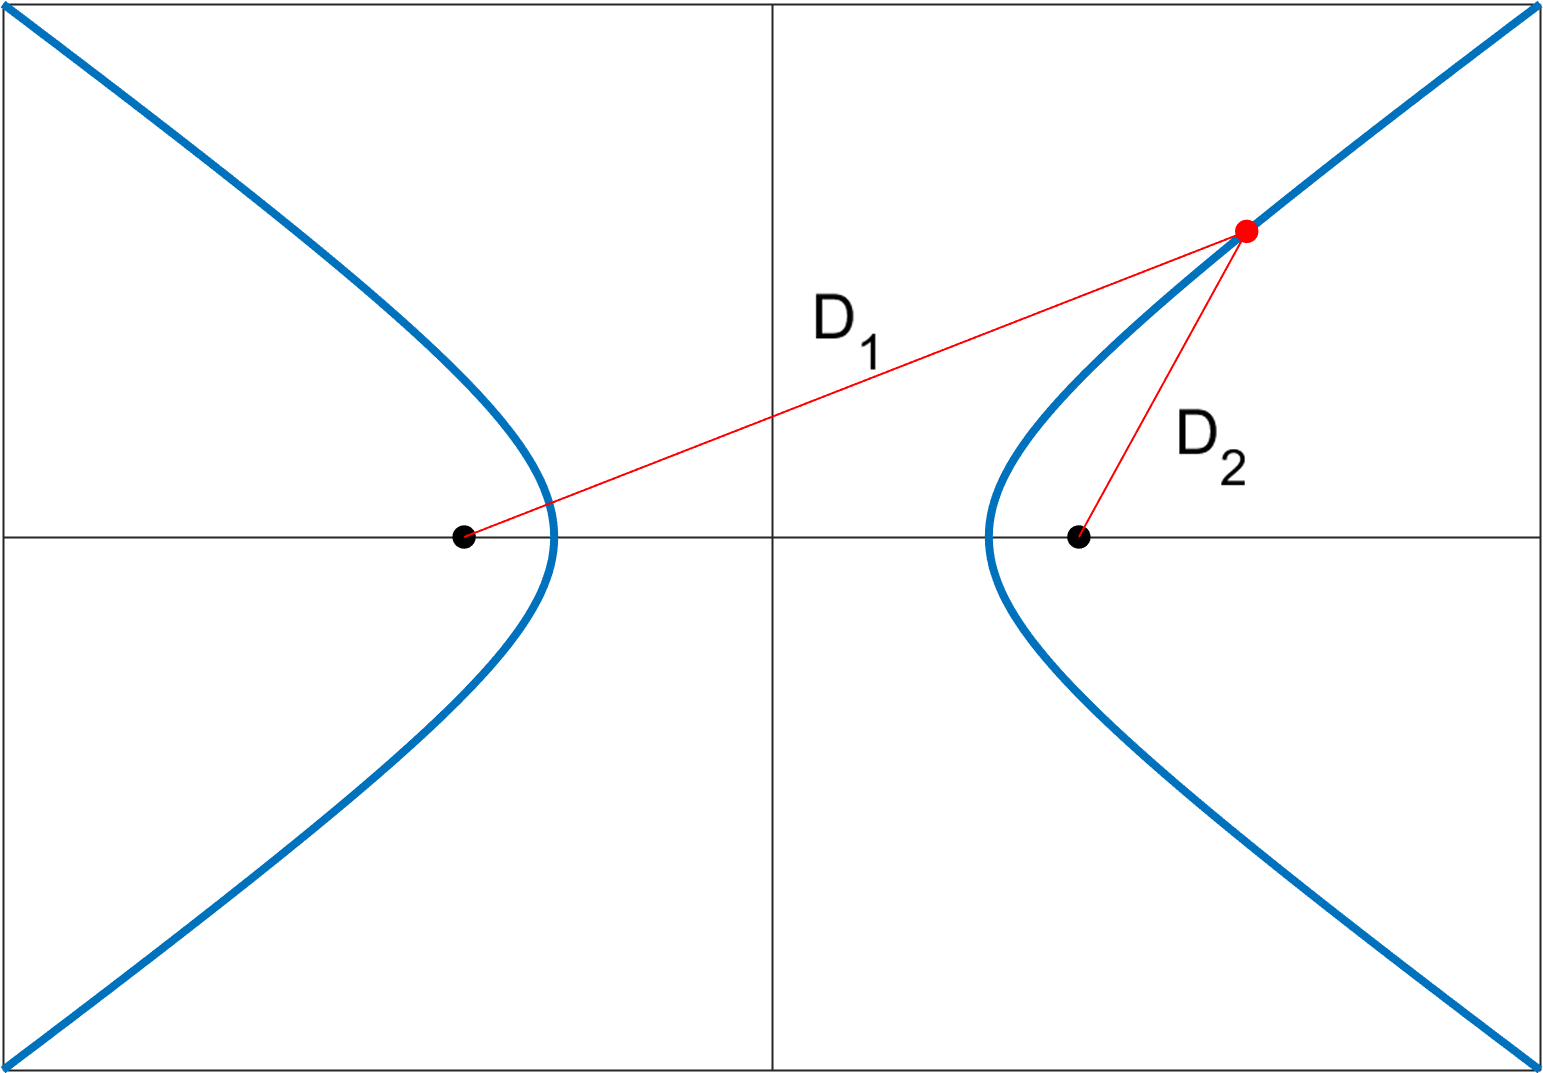
\includegraphics[width=0.8\textwidth]{Figures/hyperbola.png}
    \caption{A hyperbola (represented in blue), the red dot is any point on the hyperbola, the black dots represent the two foci. For any point on the hyperbola, $|D_1|-|D_2| = constant$}
    \label{eq:tdoa}
\end{figure}

In 3D, the TDOA information can be used to locate the source on a two-sheeted hyperboloid $\chi(\{m_{1},m_{2}\},s)$ such that the microphone positions are its foci. In practice the two-sheeted hyperboloid can be approximated to a cone so as to have a much simpler equation for the locus: $\theta$  = \textit{constant}, where $\theta$ is the angle of the source to the  midpoint of the line segment joining the two microphones (Fig. \ref{fig:hyperboloid_Cone}).

\begin{figure}[H]
    \centering
    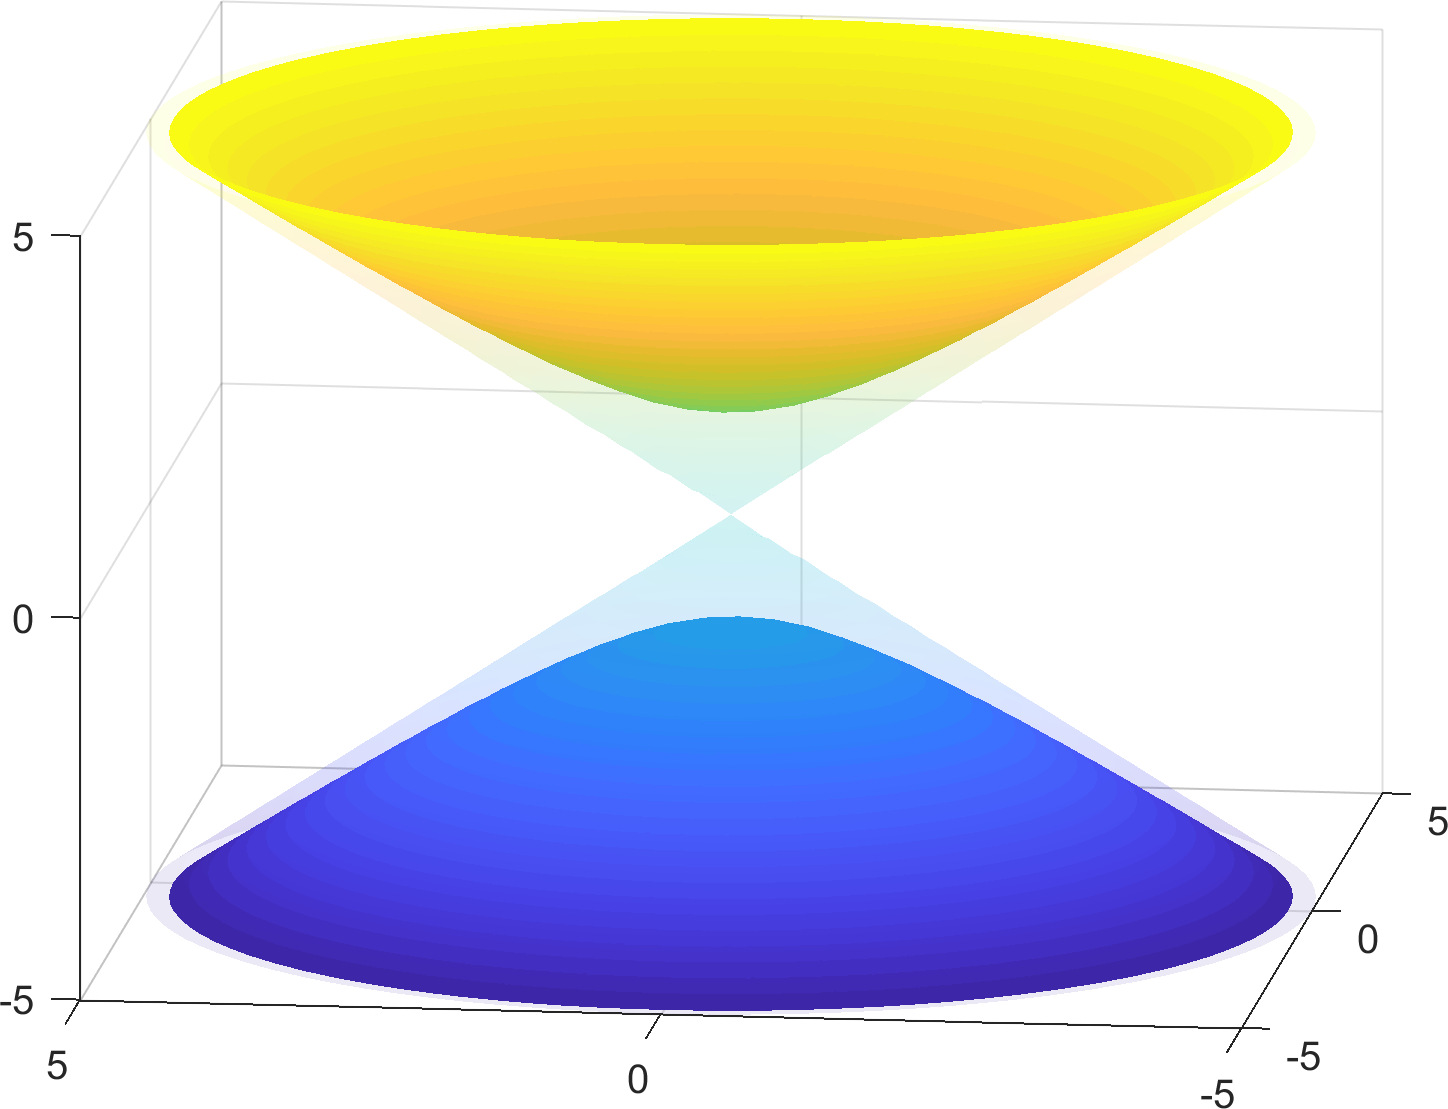
\includegraphics[width=0.8\textwidth]{Figures/hyperboloid.png}
    \caption{A 2-sheeted hyperboloid with a cone approximation overlay. As the tips of the hyperbola get closer (the microphones are closer), the hyperbola approximates the cone better.}
    \label{fig:hyperboloid_Cone}
\end{figure}

Of course as the source location gets closer to being orthogonal to the midpoint of the line segment joining the two microphones ($\theta=90\degree$), the hyperbola gets wider and flatter (more planar) and approximates the cone better. Also as the source gets closer to the line joining the two microphones ($\theta=0\degree, 180\degree$), the hyperbola collapses to a straight line and approximates the cone better. Thus, the error minimizes for broad-side sound source ($\theta=90\degree$) and for end-side sound source ($\theta=0\degree, 180\degree$), and maximizes for the midsection ($\theta=45\degree, 135\degree$). The equation for the error is given by
\begin{equation}
\begin{split}
    max\{\theta_{error}\} \approx  \frac{M_{dist}^2}{16R^2}\\
    max\{D_{error}\} \approx  \frac{M_{dist}^2}{16R},
\end{split}
\end{equation}
where $D_{error}$ is the actual source distance error (the gap between the cone and the hyperboloid) \cite{Brandstein:1995:FSS:922154}.

Microphones in microphone arrays are usually closely spaced with respect to the actual source distance, so the cone approximation works well. In most scenarios errors due to noise from other system parameters are greater than the errors associated with this approximation. Thus, given the time delay information between a microphone pair, the source can be located at a particular direction $\theta$, associated with the cone for that time delay. 

It can be shown that the cone approximation is the same as a far-field assumption for the sound source. The far-field assumption leads to a planar wave-front for a uniform linear microphone array. Thus, for the far-field, the DOA estimation problem is essentially the same as the TDOA estimation problem.

[FIG FOR FAR FIELD HERE !!!]

Now, given the TDOA between multiple microphone pairs, the source localization problem can be solved by triangulation. This triangulation problem can be solved for different variables ($\theta$, Source Distance or the Time Delay itself). The next section will detail the basics of solving such a problem. 

\subsection{TDOA of N pair of microphones}\label{sec:TDOAN}

Each pair i of sensor gives a locus $\chi{i}(\{m_{i1},m_{i2}\},s)$ on which the source can be located. When more than one pair of sensor is used, the position of the source can be found at the intersection of each locus. Depending on the position of each sensor pair and the direction of arrival of the source, the intersection of all the locus could in theory be found $ ( s\in {\bigcap}_{i=0}^k \chi{i} )$. In practical, the DOA is corrupted by random noise process which influence the localization precision and therefore the locus of each microphone pair. In most case, the locus intersection is the empty set. $ ( {\bigcap}_{i=0}^k \chi{i} = \emptyset ) $


Figure \ref{fig:hyperboloid_intersect} gives a 2D representation of 3 hyperboloid intersecting. The problem is therefore how to estimate the best intersection and how does this estimation influence our TDOA. Solution to this problem are discussed in section \ref{sec:LSTDOA}

\begin{figure}[H]
    \centering
    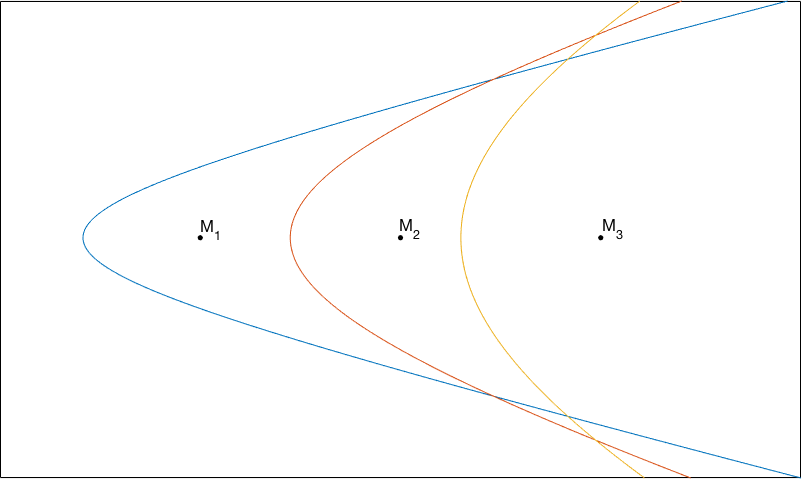
\includegraphics[width=0.8\textwidth]{Figures/intersect.png}
    \caption{2D representation of 3 locus. As seen above the intersection of the 3 locus is the empty set. $M_{1}$ , $M_{2}$ and $M_{3}$ represent the sensor position}
    \label{fig:hyperboloid_intersect}
\end{figure}

\subsection{Least Square problem}\label{sec:LSTDOA}

Let's define a Least Square (LS) problem which solves the localization of the sources in space as explained in section \ref{sec:TDOAN}. The LS problem optimize the position of the source in space by minimizing a given error criterion $ J $.
\begin{equation}
\hat{s}= \argmin_{s} J(s) 
\end{equation}

Traditionally, the literature define 3 errors criterion for solving the source location LS problem:  $J_{TDOA}(s)$, $J_{DOA}(s)$, $J_{D}(s)$. Those criterion are explains in the following sections.

\subsubsection{$J_{TDOA}(s)$ Error Criterion}

$J_{TDOA}(s)$ is the squared error difference between the time delay estimate $\tau$ and the time delay measured between the microphone pairs. The criterion and the optimization problem is given in the following.

\begin{equation}
J_{TDOA}(s) = {\sum}_{i=0}^k \epsilon_{itdoa}.[\tau_{i}-T(\{m_{i1},m_{i2}\},s)]^2
\label{eq:jtdoa}
\end{equation}
\begin{equation}
\hat{s}_{tdoa}= \argmin_{s} J_{tdoa}(s) 
\end{equation}

Assuming that the TDOA estimates $\tau_{i}$ are independently corrupted by zero-mean white gaussian noise, the stochastic variable $\mathcal{T}_{i}$ associated with this random process follows a normal distribution. The likelihood function of such a distribution is well-known and therefore the log of the distribution likelihood can be maximized yielding the Maximum Likelihood (ML) estimate of the TDOA from which the estimated position can be computed . 

Note that the error criterion is scaled by a factor $\epsilon_{itdoa}$ which is the inverse of the TDOA estimate $\mathcal{T}_{i}$ variance. 

\begin{equation}
\epsilon_{itdoa}=\frac{1}{\mathrm{Var}{\mathcal{T}_{i}}}
\label{eq:epsilonjtdoa}
\end{equation}

\subsubsection{$J_{DOA}(s)$ Error Criterion}

This is a classical formulation of the problem, which follows the same idea as the TDOA error criterion but this time the $J_{DOA}(s)$ is the squared error difference between the DOA estimate $\theta$ and the DOA measured between the microphone pairs. 

\begin{equation}
J_{DOA}(s) = {\sum}_{i=0}^k \epsilon_{idoa}.[\Theta_{i}-\theta(\{m_{i1},m_{i2}\},s)]^2
\label{eq:jdoa}
\end{equation}
\begin{equation}
\hat{s}_{doa}= \argmin_{s} J_{doa}(s) 
\end{equation}


Assuming that the DOA estimates $\theta_{i}$ are independently corrupted by zero-mean additive white Gaussian noise, the stochastic variable $\Theta_{i}$ associated with this random process follow a normal distribution. The error criterion is also scaled by a factor $\epsilon_{idoa}$ which is the inverse of the DOA estimate $\Theta_{i}$ variance. 

\begin{equation}
\epsilon_{idoa}=\frac{1}{\mathrm{Var}{\Theta_{i}}}
\label{eq:epsilonjtdoa}
\end{equation}

\subsubsection{$J_{D}(s)$ Error Criterion}

finally, $J_{D}(s)$ is the squared error difference between the orthogonal distance from s to the appropriate cone approximation 

\begin{equation}
J_{DOA}(s) = {\sum}_{i=0}^k \epsilon_{id}.[D(\chi_{i},s)]^2
\label{eq:jd}
\end{equation}
\begin{equation}
\hat{s}_{d}= \argmin_{s} J_{d}(s) 
\end{equation}


\begin{equation}
D(\chi_{i},s)=R_{i}.\sin{[\theta_{i}-\Theta(m_{i1},m_{i2},s)}]  
\end{equation}

\begin{equation}
 \epsilon_{id}=\frac{1}{\mathrm{Var}{\Theta_{i}}}    
\end{equation}

\subsubsection{Estimator performance}

The estimators described above vary in term of performance under certain conditions. For a bi-linear array, Brandstein has shown that $J_{TDOA}(s)$ and $J_{DOA}(s)$ are more robust to great angle of incidence than $J_{D}(s)$. At low noise level, $J_{TDOA}(s)$ is proven to be slightly better than $J_{DOA}(s)$ but $J_{DOA}(s)$ perform better overall especially for long range source location. $J_{TDOA}(s)$ is better for broadside sources and low noise level but $J_{DOA}(s)$ is more robust for less favorable noise conditions

%Pros and Cons of each estimators are sumarized in the following table.
\section{Methods}
\subsection{Generalized correlation method}
The famous Knapp-Carter paper details the generalized cross-correlation method (GCC) for estimation of time delay \cite{1162830} in free field. For a pair of microphones, $m_1$ \& $m_2$, separated by a distance, the signals from a source received at time t can be given by
\begin{equation}
    \begin{split}
        x_1(t) &= s_1(t) + n_1(t) \\
        x_2(t) &= \alpha s_1(t - D) + n_2(t) ,
    \end{split}
\end{equation}
where $n_1(t)$ \& $n_2(t)$ are the noise at time t at the two microphones which are uncorrelated to the signal $s_1(t)$. The microphone $m_1$ receives the signal $s_1(t)$ first, while the microphone $m_2$ receives a delayed and attenuated version $\alpha s_1(t - D)$ at time t. The $\alpha$ depends on the microphone relative distance and microphone calibration and within-media factors like absorption. The time delay D depends on the microphone pair relative distance, the speed of sound in the media and the position of the sound source. 

Based on the discussions in previous sections, if we can estimate the value of D, we can estimate the source location. However, depending on source movement and environmental factors, both $\alpha$ and D can change over time. The estimation of D thus can only be made for observations of a finite duration. D can be estimated by computing the cross-correlation of the two signals
\begin{equation}
        R_{x_1x_2}(\tau) = \textbf{E[}x_1(t)x_2(t+\tau)\textbf], 
\end{equation}
Assuming noise to be uncorrelated to each other as well as the source signal, the cross correlation can be expressed as
\begin{equation}
    \begin{split}
        R_{x_1x_2}(\tau) &= \textbf{E[}\{s_1(t) + n_1(t)\}\{\alpha s_1(t+\tau - D) + n_2(t)\}\textbf] \\
                         &= \alpha\textbf{E[}s_1(t)s_1(t+\tau - D)\textbf] \\
                         &= \alpha R_{s_1s_1}(\tau - D),
    \end{split}
    \label{Eq:crosscorr}
\end{equation}
this cross-correlation peaks at $\tau - D = 0$, i.e. $\tau = D$. So the $\tau$ that maximizes the cross-correlation is an estimator for the time delay D. Assuming the processes to be ergodic so that the samples from a finite duration T can be used to estimate the cross-correlation, the estimate can be given by
\begin{equation}
    \hat{R}_{x_1 x_2}(\tau) = \frac{1}{T-\tau}\int_{0}^{T-\tau}x_1(t)x_2(t+\tau)dt,
\end{equation}
choosing sample mean as the estimator. Notice that even though the observation interval is T, we can only get usable information for time T - $\tau$, as we will have no corresponding signal for microphone $m_2$ for any signal that we receive at microphone $m_1$ after that time.

Taking the Fourier transform of Eq. \ref{Eq:crosscorr} to move to the frequency domain
\begin{equation}
        G_{x_1x_2}(f) = \alpha G_{s_1s_1}(f)\cdot e^{-j2\pi fD},
        \label{Eq:Gx1x2Gs1s1}
\end{equation}
multiplication with $e^{-j2\pi fD}$ in the frequency domain becomes convolution in the time domain
\begin{equation}
        R_{x_1x_2}(\tau) = \alpha R_{s_1s_1}(\tau) \circledast\delta(\tau - D),
        \label{Eq:Rx1x2}
\end{equation}
which can be seen as the Fourier transform of the signal spectrum spreading the delta function. The way to ensure no spreading takes place is to use a white noise signal. The autocorrelation of white noise is a delta function, in which case convolution with the delay-delta function results in a single peak value. Of course, in any kind of a reverberant field this will never be a single value. This is because the reverberations will have the effect of making the signal add up in a periodic and attenuated manner. However, the peak of the autocorrelation $R_{x_1x_2}(\tau)$ still happens at $\tau = D$, with the spreading having the effect of broadening the peak. If the time delay D is not a single value however, as can be the case in reverberant fields or for periodic signals, the $R_{x_1x_2}(\tau)$ will have multiple peaks. Each broad peak will overlap with the other in an additive or destructive manner making is impossible to detect or distinguish peaks. 

$R_{s_1s_1}(\tau)$ in Eq. \ref{Eq:Rx1x2} can be expanded to frequency domain to get
\begin{equation}
        R_{x_1x_2}(\tau) =  {\bigg[\int_{-\infty}^{\infty}\alpha{G}_{s_1s_1}(f) e^{-j2\pi f\tau} df\bigg]} \circledast\delta(\tau - D),
\end{equation}
this cross-correlation $R_{x_1x_2}(\tau)$ is a function that is spread around $\delta(\tau - D)$ according to ${G}_{s_1s_1}(f)$. This spreading is detrimental to the resolution of the localization results. Also, if the signal itself is non-stationary, like speech signals, this spreading is also unpredictable.

Now we are ready to form a basis for the different GCC weighing methods. If \textit{a priori} signal or noise information is available, the signals  $x_1(t)$ \& $x_2(t)$ can be pre-filtered to improve the accuracy of estimating the time delay. The method of selection of the pre-filter weights then forms the basis for the different GCC methods. 

Suppose, $x_1(t)$ \& $x_2(t)$ are filtered through filters $H_1(f)$ and $H_2(f)$, to get filtered signals $y_1(t)$ \& $y_2(t)$ respectively, then we have
\begin{equation}
        G_{y_1y_2}(f) = H_1(f)H^*_2(f) G_{x_1x_2}(f),
\end{equation}
taking the Fourier transform
\begin{equation}
\begin{split}
            R_{y_1y_2}(\tau) &= \int_{-\infty}^{\infty}H_1(f)H^*_2(f) G_{x_1x_2}(f) e^{-j2\pi f\tau} df \\
                             &= \int_{-\infty}^{\infty}\psi(f) G_{x_1x_2}(f) e^{-j2\pi f\tau} df,
\end{split}
\end{equation}
where 
\begin{equation}
            \psi(f) = H_1(f)H^*_2(f),
\end{equation}
since we can only estimate the cross-power spectra, we can write
\begin{equation}
            \hat{R}_{y_1y_2}(\tau) = \int_{-\infty}^{\infty}\psi(f) \hat{G}_{x_1x_2}(f) e^{-j2\pi f\tau} df,
\end{equation}
the frequency weights given by $\psi(f)$ can be selected according to the purpose that is wished to be achieved. For example, if the purpose is to maximize the signal-to-noise (SNR) ratio in the signal passed, then the $\psi(f)$ could be selected so that it attenuates the frequencies in the noise spectra. Obviously this requires either priori-knowledge or estimation of the noise spectra. The following sections introduce the different methods of frequency weight selection. Four methods are described here, ROTH, SCOT, PHAT and ML. Of particular interest are the PHAT and ML, direct and improved versions of which have been consistently used to do robust source localization. 

\subsubsection{ROTH}
The frequency weights for ROTH processor are defined as
\begin{equation}
            \psi(f) = \frac{1}{G_{x_1x_1}(f)},
\end{equation}
so we get 
\begin{equation}
            {R}_{y_1y_2}(\tau) = \int_{-\infty}^{\infty}\frac{{G}_{x_1x_2}(f)}{G_{x_1x_1}(f)} e^{j2\pi f\tau} df,
\end{equation}
substituting the value for ${G}_{x_1x_2}(f)$ assuming uncorrelated noise from Eq. \ref{Eq:Gx1x2Gs1s1} we get
\begin{equation}
\begin{split}
                \hat{R}_{y_1y_2}(\tau) &= \int_{-\infty}^{\infty}\frac{\alpha\hat{G}_{s_1s_1}(f)}{G_{x_1x_1}(f)} e^{j2\pi f.(\tau-D)} df \\
                                        &= \delta (\tau - D) \circledast \bigg[\int_{-\infty}^{\infty}\frac{\alpha\hat{G}_{s_1s_1}(f)}{G_{s_1s_1}(f) + G_{n_1n_1}(f)} e^{j2\pi f\tau}  df\bigg],
                                        %&= \delta (\tau - D) \circledast \alpha\bigg[\int_{-\infty}^{\infty}\frac{{G}_{s_1s_1}(f) + G_{n_1n_1}(f) -G_{n_1n_1}(f)}{G_{s_1s_1}(f) + G_{n_1n_1}(f)} e^{j2\pi f\tau}  df\bigg] \\
                                        %&= \delta (\tau - D) \circledast \alpha\bigg[\int_{-\infty}^{\infty}e^{j2\pi f\tau}df-\int_{-\infty}^{\infty}\frac{G_{n_1n_1}(f)}{G_{s_1s_1}(f) + G_{n_1n_1}(f)} e^{j2\pi f\tau}  df\bigg] \\
\end{split}
\end{equation}
so now the delta function is spread according to the value of $G_{n_1n_1}(f)$. For frequencies f where $G_{n_1n_1}(f)$ has a high magnitude, the cross-correlation will be suppressed, so that peaks in the frequency regions where $n_1$ is high disappear. But as can be seen ROTH processor does nothing to improve the high $n_2$ regions or the spreading around the main peak.

\subsubsection{SCOT}
The frequency weights for SCOT processor are defined as
\begin{equation}
            \psi(f) = \frac{1}{\sqrt{G_{x_1x_1}(f)G_{x_2x_2}(f)}},
\end{equation}
so this takes care of regions where either $n_1$ or $n_2$ might be high solving a possible disadvantage with ROTH. 

\subsubsection{PHAT}
Both SCOT and ROTH suffer from the disadvantage that the value of ${R}_{y_1y_2}(\tau)$ is spread around the delta function depending on the cross-spectrum ${G}_{x_1x_2}(f)$. However, the TDOA information is carried only by the phase of the cross-spectrum and not the amplitude. So, setting the weights as
\begin{equation}
            \psi(f) = \frac{1}{|G_{x_1x_2}(f)|},
\end{equation}
we get
\begin{equation}
        {R}_{y_1y_2}(\tau) = \int_{-\infty}^{\infty}\frac{{G}_{x_1x_2}(f)}{|G_{x_1x_2}(f)|}e^{j2\pi f\tau}   df,
\end{equation}
Now, we have from Eq. \ref{Eq:Gx1x2Gs1s1}
\begin{equation}
\begin{split}
        |G_{x_1x_2}(f)| &= \alpha G_{s_1s_1}(f) \\
    \frac{{G}_{x_1x_2}(f)}{|G_{x_1x_2}(f)|}&=e^{-j2\pi fD},
\end{split}
\label{Eq:ModGx1x2}
\end{equation}
where the magnitude information is cancelled and only the phase information remains, where D is the delay or the 'phase'. We get
\begin{equation}
\begin{split}
            {R}_{y_1y_2}(\tau) &= \int_{-\infty}^{\infty}e^{j2\pi f(\tau - D)}   df \\
                           &=  \delta (\tau - D) \circledast \int_{-\infty}^{\infty}e^{j2\pi f\tau} df,
\end{split}
\label{Eq:RY1Y2}
\end{equation}
So ideally PHAT weighing gives a cross-correlation value that has no spreading and gives a clean peak at $\tau=D$.

Even though PHAT seems to solve all problems, the method is not without issues. Most of the issues arise from the assumptions made for PHAT. These are itemized below: 
\begin{itemize}
    \item $n_1$ and $n_2$ are assumed to be uncorrelated. If that is not the case, the magnitude of $G_{x_1x_2}(f)$ would obviously not cancel out in Eq. \ref{Eq:ModGx1x2}
    \item The GCC methods assume single-source in free-field model, ie, no reverberation is assumed. The effects of reverberation can actually be moderate to severe in PHAT and have been discussed in various papers [Cite papers here]. 
    \item The 'expected' value of $G_{x_1x_2}(f)$ is assumed to be known. In reality it can only be estimated, viz $\hat{G}_{x_1x_2}(f)$. In situations where $\hat{G}_{x_1x_2}(f) \neq G_{x_1x_2}(f)$, the cross-correlation in Eq. \ref{Eq:RY1Y2} will not be a delta function. This error is magnified even more in regions where $G_{s_1s_1}(f)$ is very low. This has the potential to cause PHAT to provide poor results in low SNR conditions.
\end{itemize}  

A practical issue that exists with GCC methods is the angular resolution of localization. If the signals are recorded at 44.1kHz sample rate, then the minimum time delay allowed is $1/$ 44100 sec for 1 sample delay. For 2 microphones placed distance $20$ cm apart, the minimum resolution achievable in this time is $2.2\degree$ broadside to $16\degree$ endside, assuming speed of sound to be 343 m/sec (Fig. \ref{fig:ang_res}). At 192kHz and 1m microphone distance, the issue is less severe, being $0.5\degree$ broadside to $7.7\degree$ endside.
\begin{figure}[H]
     \centering
     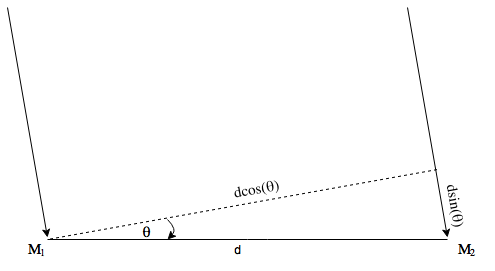
\includegraphics[width=0.8\textwidth]{Figures/AngularRes.png}
     \caption{Figure represents plane wave incidence on a microphone pair. For broadside incidence the time delay is the minimum = 0 between the two microphones. The next time delay allowed is $1/$fs, corresponding to travel distance of $c/$fs (c being the speed of sound). So we have  dsin($\theta$) = $c$/fs. For endside incidence the time delay is maximum = $d/c$. The next time delay allowed is $d/c$-$1/$fs, corresponding to travel distance of $d$-$c/$fs, and we have dsin($\theta$) =  $d$-$c/$fs.}
     \label{fig:ang_res}
\end{figure}

The issue is solved by curve fitting and interpolation. Parabolic curve fitting was initially proposed method to solve it, but was shown to be a biased estimator \cite{boucher1981analysis}. Consequently, various interpolation techniques have been developed to overcome this issue \cite{jacovitti1993discrete}, \cite{brandstein1997practical}, \cite{zhang2005cross}, \cite{tervo2008interpolation}. The 2D localization resolution with no interpolation is plotted in Fig. \ref{fig:res_diff}.

\begin{figure}[H]
    \centering
    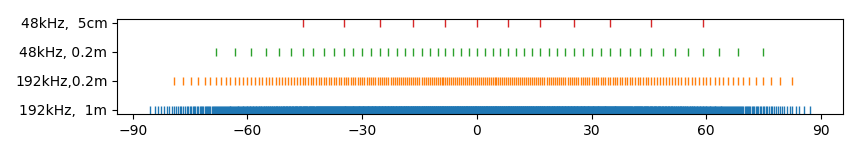
\includegraphics[width=\textwidth]{Figures/res_diff.png}
    \caption{Frontal 2D localization resolution for different sample rates and distance between a pair of microphones. As can be seen large apertures and high sample rates have a better resolution than lower sample rates and smaller apertures.}
    \label{fig:res_diff}
\end{figure}

Some simulations for GCC are given in Fig. \ref{fig:GCC_SIM}. It can be seen that the resolution falls the closer we get to end-side ($0\degree$ and $180\degree$). Also it can be seen that the results are poor if no weights are used. PHAT and SCOT perform quite similarly in the simulations, with PHAT being marginally better. It can be seen that the level difference is maintained between the 2 sources in the results. However no peaks are visible if the SNR falls to 0 dB.

\begin{figure}[H]
    \centering
    \begin{subfigure}[b]{0.48\textwidth}
    \centering
    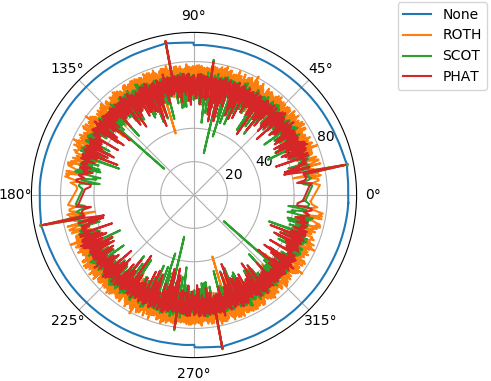
\includegraphics[width=0.9\textwidth]{Figures/GCC_40.png}
    \caption{Both sources at 40dB SNR}
    \label{fig:d1}
\end{subfigure}
\hfill
\begin{subfigure}[b]{0.48\textwidth}
    \centering
    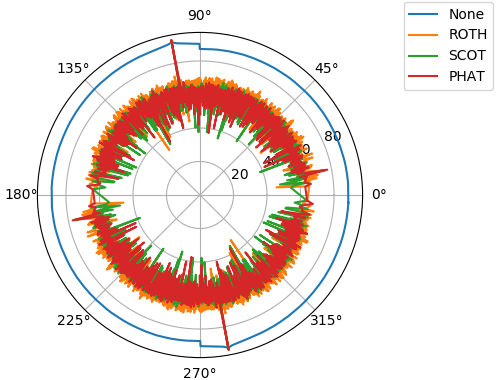
\includegraphics[width=0.9\textwidth]{Figures/GCC_20_40.png}
    \caption{S1 at 20dB SNR, S2 at 40dB SNR}
    \label{fig:d2}
\end{subfigure}
\vskip \baselineskip
\begin{subfigure}[b]{0.48\textwidth}
    \centering
    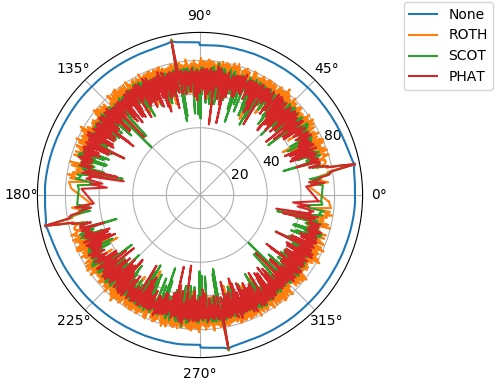
\includegraphics[width=0.9\textwidth]{Figures/GCC_20_20.png}
    \caption{Both sources at 20dB SNR}
    \label{fig:d3}
\end{subfigure}
\quad
\begin{subfigure}[b]{0.48\textwidth}
    \centering
    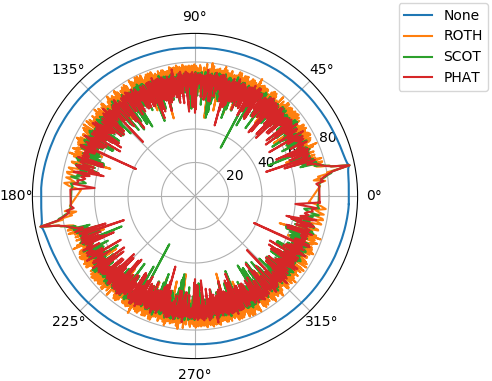
\includegraphics[width=0.9\textwidth]{Figures/GCC_0_20.png}
    \caption{S1 at 20 SNR, S2 at 0 SNR}
    \label{fig:d4}
\end{subfigure}
\caption{Figures compares different GCC algorithms for localization performance for 2 sources with various SNRs. The simulations assume 2 microphones placed 1m apart along the $0\degree-180\degree$ axis. The sampling rate is assumed to be 192kHz and speed of sound is 343m/sec. Two sources playing pink noise at different levels and located at $S_1:15\degree$ and $S_2:100\degree$ are assumed. Uncorrelated white noise is assumed to be present at the 2 microphones. No interpolation fixing is done. The level of the noise is unchanged but the level of the signal is varied to achieve the different SNRs.}
\label{fig:GCC_SIM}
\end{figure}


\subsection{Multiple pair GCC}

GCC equations described above are for a single pair of microphones only. Various algorithms have been designed that extend the GCC algorithm to multiple pairs of microphones. SRP-PHAT approach \cite{dibiase2000high} combines the steered response power (SRP) beamformer methods \cite{krim1996two} to the GCC approach. Griebel \cite{griebel2001microphone} describes a method where the \enquote{GCC functions derived from various microphone pairs are simultaneously maximized over a set of potential delay combinations consistent with candidate locations} which can be seen as a special case of SRP-PHAT where the redundant information from additional microphone pairs are utilized. \textit{Okuyama et al.} show in a 2002 study\cite{okuyama2002study} that when using a spatial array like a tetrahedron, the propagation direction of sound through the array can be determined, irrespective of the speed of sound, by using the least-squares approach. This means that for localizing sound sources outdoors, the instantaneous temperature and wind on the microphone array need not be known. Benesty \cite{benesty2004time} provides a method to fully utilize the redundant information from multiple microphone pairs to make the time-delay estimation (TDE) process more robust against distortion and also improve angular resolution. The method re-derives multi-channel cross correlation (MCCC) to apply linear interpolation on the GCC data to improve the angular resolution of localization. More recently, in \cite{liu2010continuous} the author used a motorized robot with 4 microphone arranged in a cross-formation. The algorithm uses 'de-noising' techniques such as adding a small regularization term to the denominator of the PHAT weight, which can reduce the low SNR issues surrounding PHAT. The low SNR regions can be further penalized by using reliability-weighted RW-PHAT \cite{valin2006robust}, where a-priori SNR information is used to estimate the weight to be multiplied during the PHAT computation. Eigenvalue decomposition based GCC (ES-GCC) is done by authors in \cite{hu2009estimation}. They conclude that ES-GCC produces less number of outlier locations that GCC-PHAT. Badali \cite{badali2009evaluating} compares various localization algorithms using a 8 microphone array located on a cube. The authors use hyperbolic intersection on the GCC results from multiple pairs of microphones. They conclude that if \textit{Direction Refinement} procedure is run, in which first a far-field assumption search is done and the locations are then 'refined' for near field, then the results from SRP-PHAT can be improved. But this procedure might not be relevant for far-field outdoor localization.  

The next sections will discuss some of the algorithms that are relevant for outdoor source localization and make the PHAT process more robust. 
\subsection{Steered Response Power}

Steered Response Power (SRP) source localization is a method to detect sound source locations using beamforming techniques \cite{krim1996two}. SRP is different from TDOA based methods discussed before. While the generalized cross correlation is a simple cross correlation between each pair of microphones and only outputs an estimate of the time delay, the SRP method beamforms the space around the array and computes the energy of each location beam.  It `looks' at all possible directions individually (steering) and computes the power of the signal cross correlation in that direction (beamforming). The assumption is that the cross power of the steered microphone array will be the maximum in the correct source direction. However, the computational demand for this can rise quite fast (depending on the sampling rate and the angular resolution of the beamforming), making it nearly impossible to implement in real time applications. However, its performance in difficult conditions outperforms the TDOA based methods \cite{dmochowski2007generalized}. Since real-time localization is not of primary importance for this thesis, SRP based methods can be applied. In the same fashion as the GCC method proposed to pre-filter the signal before performing the cross correlation, a PHAT weighing can be applied on the beamformed signal. This method is called SRP-PHAT. In this section, the first part discusses the basic principles behind the method whereas the second part introduces a hybrid method that improves the computational time of SRP without decreasing its robustness. 

%\subsubsection{Steered Beamformer}

The SRP method is based on a regular delay-and-sum beamformer, for a given point in space having range $\rho$, azimuth $\theta$ and elevation $\phi$ with the microphone array, the output of the beamformer is given by

\begin{equation}
    y_{\rho,\theta,\phi}(n)=\sum\limits_{m=0}^{M-1}{w_m x_m[n + f_{0,m}(\rho,\theta,\phi)]},
\end{equation}

where $x_0[n]$ is the signal received at time n, at an arbitrary microphone used as reference, $w_m$ is the amplitude weight for microphone m, and $f_{0,m}(\rho,\theta,\phi)$ is the relative delay between the reference microphone and the $m^{th}$ microphone. When far-field approximation is assumed, the range cannot be computed and the delay-and-sum beamformer output can be rewritten as follows:

\begin{equation}
    y_{\theta,\phi}(n)=\sum\limits_{m=0}^{M-1}{w_m x_m[n + f_{0,m}(\theta,\phi)]} 
\end{equation}


For $w_m=1$ (assuming perfectly omni-directional and equally sensitive microphones), the output power of the beamformer becomes

\begin{equation}
    \mathbb{E}[{y_{\theta,\phi}(n)^2}]=\sum\limits_{i=0}^{M-1}\sum\limits_{j=0}^{M-1}{R_{x_i,x_j}[f_{i,j}(\theta,\phi)]} 
    \label{eq:poweroutputbeamformer}
\end{equation}

This cross correlation is computed in the frequency domain using cross-spectrum which is then inverse fast Fourier transformed (IFFT).

\begin{equation}
    R_{x_i,x_j}(\tau)= \sum\limits_{k=0}^{N_{f}-1}{X_{i}(k)X_{j}^*(k)e^{j2\pi\frac{k}{N_{f}}\tau}}
\end{equation}

%\subsubsection{SRP Search}

The SRP method starts with a look up procedure which associates each set of angles ($\phi,\theta$) to a given set of delays between each microphone pair. For instance if we use a 1$\degree$  resolution, the SRP method associates 360*360=129600 angular positions to corresponding delays. The cross correlations of the signals received at the different microphone pairs combinations possible are then computed. For a given position ($\phi,\theta$), the output of the SRP search is simply the sum of the cross correlation at each time delay found relative to each pair of microphone. It corresponds to the power output of the beamformer defined in Eq. \ref{eq:poweroutputbeamformer}. 
\begin{equation}
    S_{SRP}(\theta,\phi)=\sum\limits_{i=0}^{M-1}\sum\limits_{j=0}^{M-1}{R_{x_i,x_j}[f_{i,j}(\theta,\phi)]}
\end{equation}

\begin{figure}[H]
    \centering
    \begin{subfigure}[t]{0.5\textwidth}
    \centering
    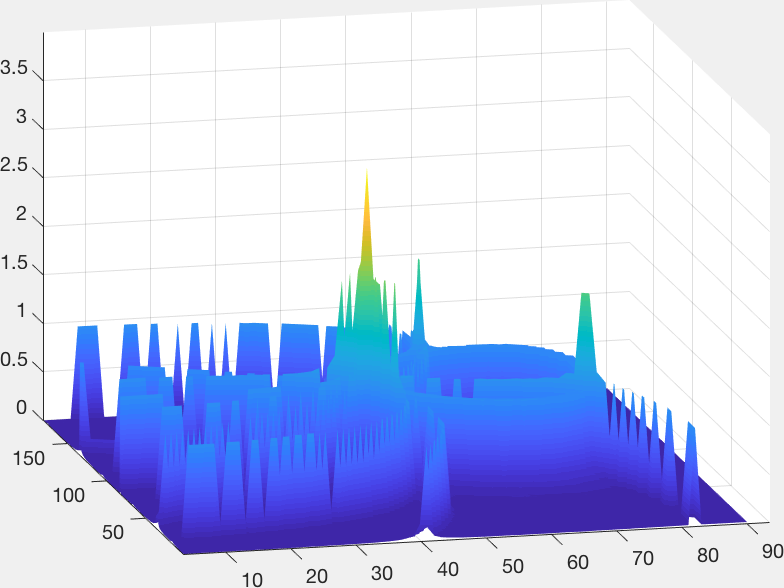
\includegraphics[width=0.9\textwidth]{Figures/viewside.png}
    \caption{SRP map}
    \label{fig:viewsidesrp}
\end{subfigure}%
\begin{subfigure}[t]{0.5\textwidth}
    \centering
    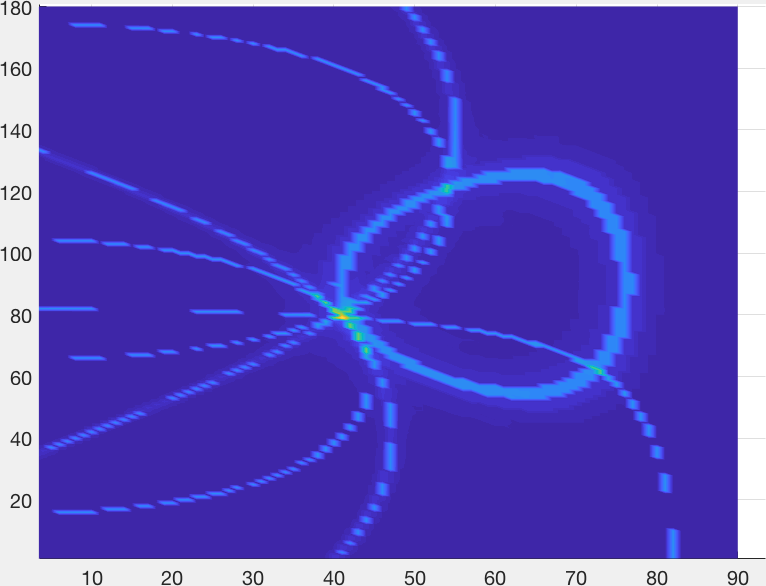
\includegraphics[width=0.9\textwidth]{Figures/topview.png}
    \caption{SRP heat map}
    \label{fig:topviewsrp}
\end{subfigure}
\caption{Power mapping simulation of source localized using SRP-PHAT algorithm in noiseless, free-field situation. For the simulation, first a 4-channel wav file is created such that the channels contain the same pink noise but delayed between each other. The delays are such that the source would be ideally located at azimuth $80\degree$ and elevation $40\degree$ when localized by a 1m aperture tetrahedral array. SRP-PHAT is then applied on the wav file and power received from different angles (beams) is computed and plotted. As can be seen the algorithm was able to localize the source in these ideal conditions fairly correctly.}
\end{figure}

The SRP method estimates the source location ($\hat{\phi},\hat{\theta}$) after creating the SRP search space such that

\begin{equation}
    \hat{\phi},\hat{\theta}=\argmax_{\phi,\theta}S_{SRP}(\phi,\theta)
\end{equation}

%\subsubsection{Premapping the delays to potential sources locations}

The classical SRP search beamforms sequentially the 3D space and locations [($\phi_{1},\theta_{1}$), ($\phi_{2},\theta_{2}$), ... ,($\phi_{x},\theta_{x}$)] which might be associated with the same relative delay $\tau_{1}$ (in case of a uniform linear microphone array). The cross correlation at delay $\tau_{1}$ is then computed $x$ times, which leads to the same results for each [($\phi_{1},\theta_{1}$), ($\phi_{2},\theta_{2}$), ... ,($\phi_{x},\theta_{x}$)] positions, leading to numerous useless cross correlation computations. In \cite{dmochowski2007generalized} the authors propose an improvement on the SRP search algorithm by pre-mapping the relative delays to their corresponding set of locations. Instead of proceeding to a sequential search in the 3D space, a search on the possible relative delays is considered. The possible delays between individual microphone pairs are already known based on the array geometry and can be stored in memory. The cross correlations are calculated for each delay subset and related to a set of potential source location in space in the final steps of the algorithm. Note that the computational cost gain can be immense depending on the number of microphones (the more the microphones, the greater the gain), the aperture size (the smaller the microphone array the more angles are associated with the same time delay) or the sampling rate (again the smaller the sampling rate the more angles are associated with the same time delay). In GCC methods this issue was taken care of by interpolation, where the microphone pair end-side localization had poor resolution (Fig. \ref{fig:res_diff}). 

The method can be easily extended to SRP-PHAT, where pre-filtering the signal beforehand by using PHAT introduces a function $\psi_{ij}$ in the cross correlation

\begin{equation}
    R_{x_i,x_j}(\tau)= \sum\limits_{k=0}^{N_{f}-1}{\psi_{ij}(k) X_{i}(k)X_{j}^*(k)e^{j2\pi\frac{k}{N_{f}}\tau}}
\end{equation}
where
\begin{equation}
    \psi_{ij}(k) = \frac{1}{|{X_{i}(k)X_{j}^*(k)}|}
\end{equation}

\subsubsection{Simulations}

Two identical sound sources are placed in the far field. A tetrahedral array with equal spacing between microphones of 1 meter is receiving the two sources. The sound received at the sources are 3 seconds of two different pink noises with respective DOA $\tetha_{1}=120\degree$, $\phi_{1}=40\degree $ and $\tetha_{2}=150\degree $ , $\phi_{2}=75\degree $. Waves are propagating in free field where no reflections and no noise is added to the microphones. The SRP maps are computed and displayed in the figure \ref{fig:coherent2pinknoise}. Source 2 is placed at a problematic angle for the tetrahedral array, detection errors are discussed in section \ref{sec:detection}. Error probability increases as the source DOA approach the angle of the axis drawn by pairs of microphones (end-side).

\begin{figure}[H]
    \centering
    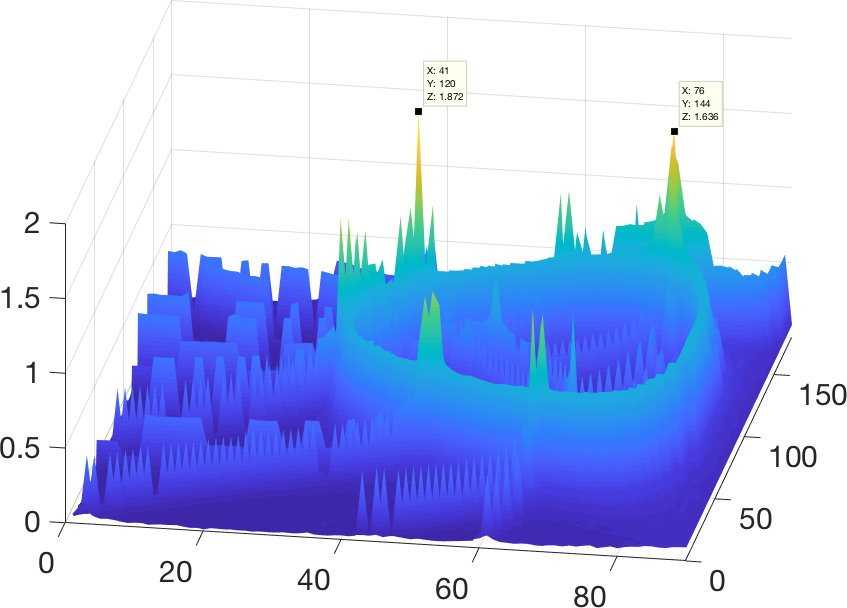
\includegraphics[width=1\textwidth]{Figures/2pinknoisesrpphat.png}
    \caption{SRP-PHAT simulation with 2 sound sources localized using a tetrahedral array}
    \label{fig:coherent2pinknoise}
\end{figure}

\subsubsection{Localization errors} \label{sec:detection}

Two pairs of microphones are considered, the axes drawn by the two pairs is plotted (extended) in figure \ref{fig:locerrortetra}. The two axes form respective angles of $45\degree$ and $60\degree$ with the horizontal axis. Plane waves with DOA between $45\degree$ and $60\degree$ will cross the two pairs of microphones at an angle close to the respective end-sides of the pairs. As shown in figure \ref{fig:errorsimulation1} maximum errors arise in the simulation for DOA contained in between $45\degree$ and $60\degree$. For a tetrahedral array, this can be seen as the 3d space created by extending the arms connecting the microphones. 

\begin{figure}[H]
    \centering
    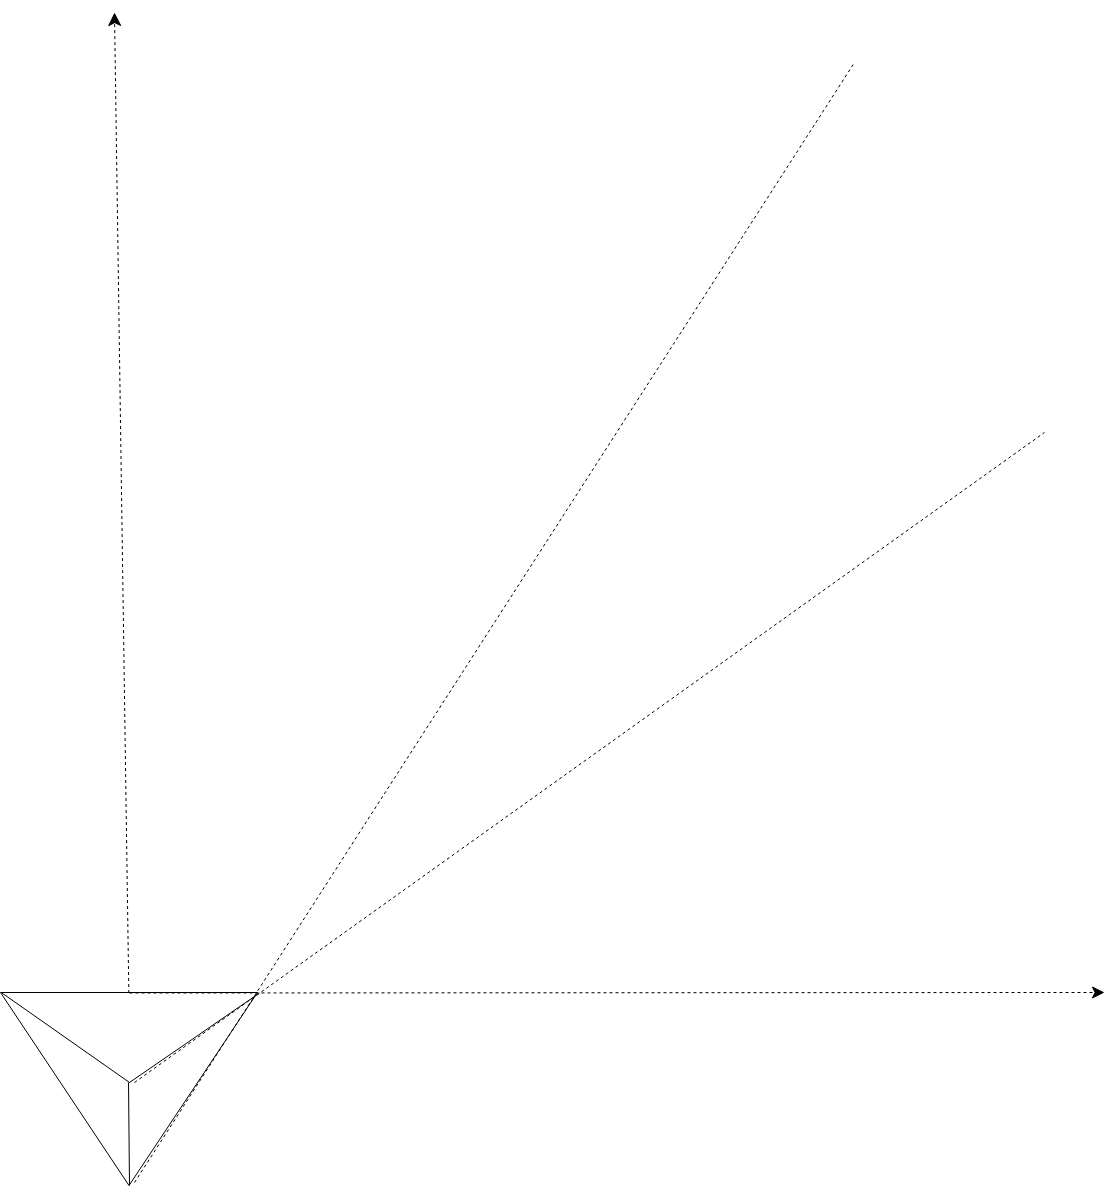
\includegraphics[width=0.9\textwidth]{Figures/locerrors.png}
    \caption{Axis drawn by 2 pairs of microphones}
    \label{fig:locerrortetra}
\end{figure}

\begin{figure}[H]
    \centering
    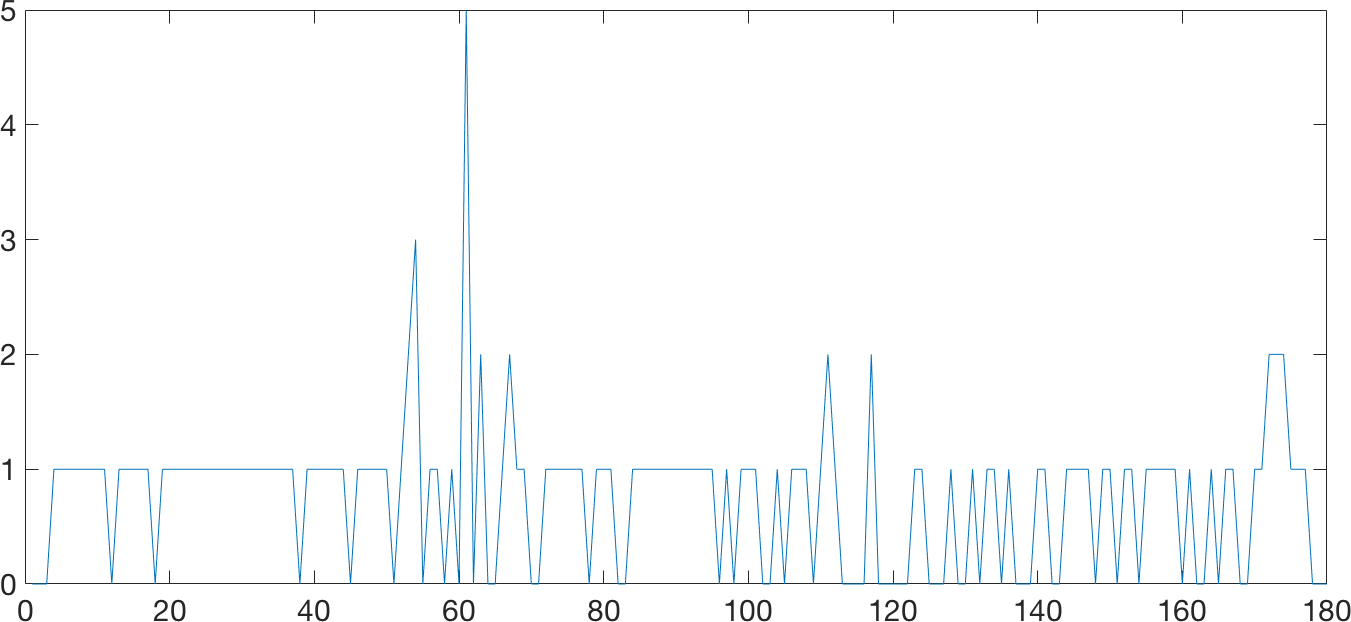
\includegraphics[width=0.9\textwidth]{Figures/errorphinointerpolationandrounding.png}
    \caption{Simulation errors with no interpolation}
    \label{fig:errorsimulation1}
\end{figure}

\subsection{Hybrid SRP-PHAT}

Peterson \cite{peterson2005hybrid} describes a novel approach for sound localization using a two stage approach in order to reduce the computational load. The first stage roughly identifies the sources locations while the second stage is a modified version of the SRP-PHAT algorithm that only performs a grid search around the estimated location from the first stage.  The method is well suited for near-field localization using large aperture array which is not our requirement but the idea can be adapted in the case of far-field sound localization. Section \ref{sec:TDOA} gives an introduction to TDOA based localization and introduces the cone approximation for the far-field. The idea of the hybrid approach is to do a classical GCC-PHAT estimation to get the relative delays between the sensors. The delays estimates are used to derive the cone intersections which give a location estimate which is then input into a SRP-PHAT algorithm where the search region is constrained around the location estimates. A system overview of the algorithm is given in figure \ref{fig:hybridalgo}.

\begin{figure}[H]
    \centering
    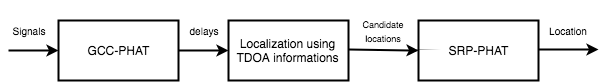
\includegraphics[width=1\textwidth]{Figures/hybridalgo.png}
    \caption{Simplified block diagram of the Hybrid algorithm}
    \label{fig:hybridalgo}
\end{figure}

\subsection{Improvements on SRP}

In \cite{salvati2017exploiting} the author proposes a method to improve the computational efficiency and coherence of the grid search using discreet sampling information where the method is called geometrically sampled grid (GSG). \cite{do2007real} uses Stochastic Region Contraction(SRC) to reduce the computational time of the search. \cite{salvati2014incoherent} introduces an incoherent Frequency Fusion based on a normalized arithmetic mean (NAM) which improves the localization performance of SRP, MVDR and MUSIC. Paper \cite{salvati2015frequency} introduces a SRP weighted MVDR, which combines machine learning power to the noise resilience of the MVDR beamformer, the method is improved in \cite{salvati2016use} by using SVM training. SRP-WMVDR is proved to be much more resilient to noise and better than SRP-PHAT for SNR up to 0. All of those papers uses a microphone array composed of mostly more than 8 microphones. Few experiment data are available for the case of 4 microphones and none for the case of a tetrahedral array, whereby a ULA is mostly used for the different test methods.



\section{Far-field sound localization using minimum-power SRP-PHAT}


\subsubsection{Using the redundant information from the microphone pairs}
A thing to note is that Eq. \ref{Eq:linearDep} is only true for no noise conditions. In case of low SNR, there is a potential to gain information by using the redundant microphone pairs. This is because if noise at all microphones is assumed to be uncorrelated, even though noise causes some microphone pairs to detect a source at a 'sourceless` location of the SRP search, certain microphone pairs will have a lower magnitude at that location. So in case of a SRP-PHAT, the sum of all microphone pairs will be higher at the real source location, and at other locations, the sum due to the noise will be suppressed. Fig. \ref{fig:4mic1srcRedun} shows the effect of using all microphone pairs for noisy conditions. Note that the dynamic range in the figure has been lowered to highlight the differences. It can be seen that using all the microphone pairs adds to the overall noise as more pairs can now contribute to the SRP sum, however, ideally the peak of the true source would also be higher, due to more pairs providing power at the source location. 
\begin{figure}[H]
\begin{subfigure}[b]{0.96\textwidth}
    \centering
    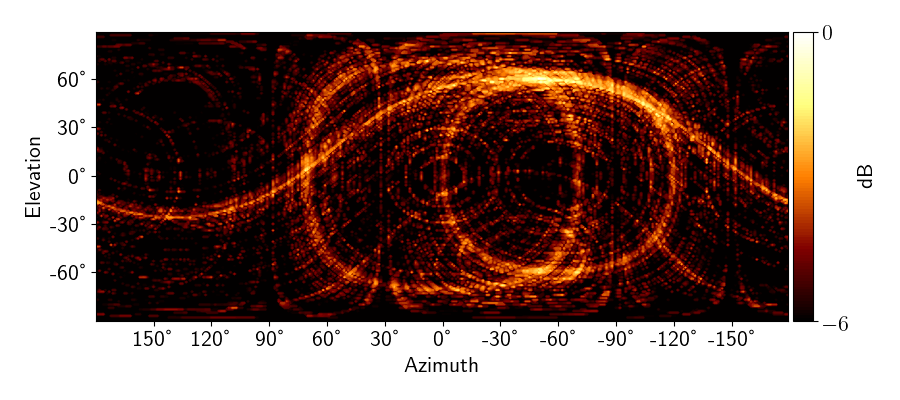
\includegraphics[width=0.8\textwidth]{Figures/Ind4mic1srcResNeg10LowDyn.png}
\end{subfigure}
\vskip \baselineskip
\begin{subfigure}[b]{0.96\textwidth}
    \centering
    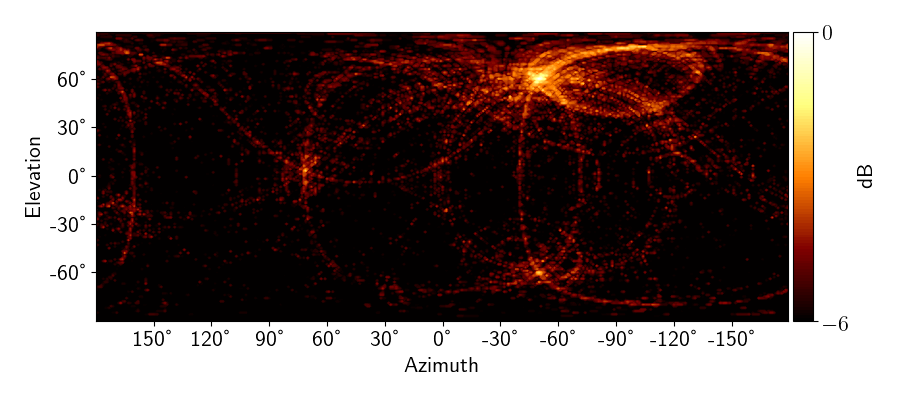
\includegraphics[width=0.8\textwidth]{Figures/Dep4mic1srcResNeg10LowDyn.png}
\end{subfigure}
\caption{Figures depict from SRP-PHAT localization results with SNR = -10dB, for independent microphone pairs (top), and for all  microphone pairs (bottom)}
\label{fig:4mic1srcRedun}
\end{figure}







\subsection{Deconvolution of the array response}

As can be seen in fig. \ref{fig:4mic1srcInd}, even in ideal conditions, the localization results from SRP-PHAT contain many peaks of varying heights. This is due to summing the cross-correlation responses of a non-linear array (Eq. \ref{eq:srpSumInd}). If the array was linear, the localization circles from each pair would all overlap completely. In case of a tetrahedral array, the localization circles from the possible microphone pairs are not co-planar. This is because all the edges of a tetrahedron point in the different directions. The obvious problem here is in multi-source detection. If multiple sources are playing at different levels, how do we determine if a detected peak is a real source or a pseudo-source from another higher level source? The methods to do so form the basis of deconvolution methods for SRP-PHAT.

\subsection{Deconvolution history}
Coming Soon!
\newpage
\subsubsection{Product-SRP-PHAT}
A simple deconvolution approach could be to penalize sources which are only detected by a subset of the microphone pair combinations. This could be done by taking a product and not a sum in Eq. \ref{eq:srpSumInd}.
\begin{equation}
    S_{SRP}(\theta,\phi)=\prod\limits_{i=1}^{M-1}{R_{x_0,x_i}[f_{0,i}(\theta,\phi)]}
     \label{eq:srpProdInd}
\end{equation}
This way, if a peak is caused by a single localization circle, the cross-correlation values from other microphone pairs would be close to zero, and thus would scale the false peak down. The localization results from this are given in fig. \ref{fig:4mic1srcNoisyProd}.
\begin{figure}[H]
    \centering
    \begin{subfigure}[b]{0.96\textwidth}
    \centering
    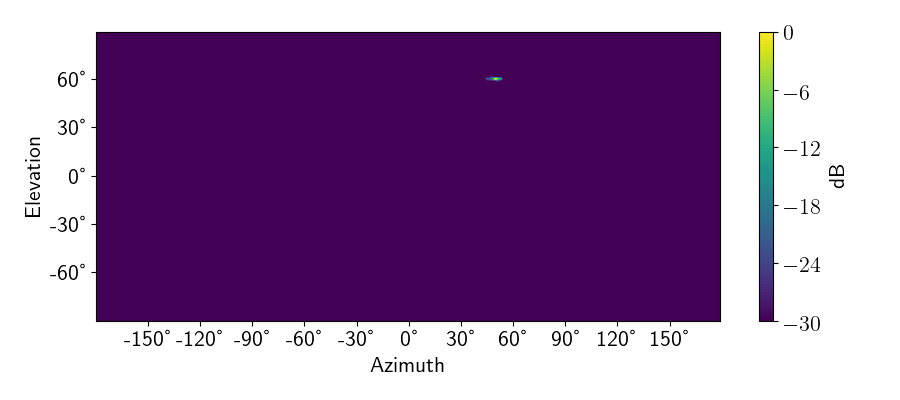
\includegraphics[width=0.8\textwidth]{Figures/Ind4mic1srcProd20.png}
\end{subfigure}
\vskip \baselineskip
\begin{subfigure}[b]{0.96\textwidth}
    \centering
    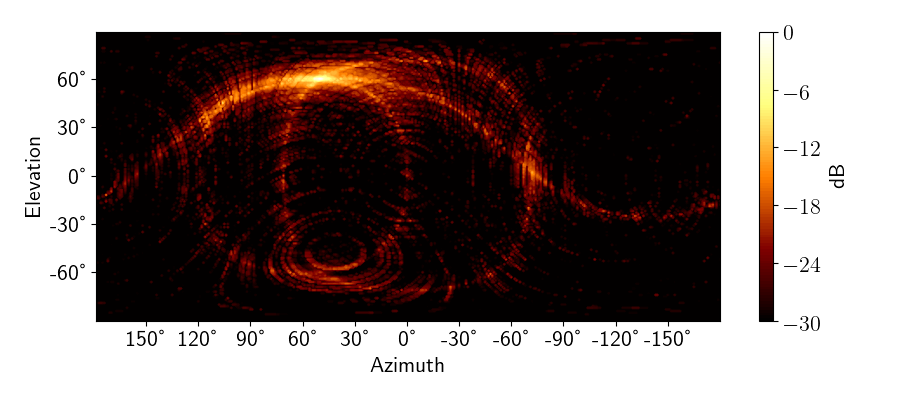
\includegraphics[width=0.8\textwidth]{Figures/Ind4mic1srcProd0.png}
\end{subfigure}
\vskip \baselineskip
\begin{subfigure}[b]{0.96\textwidth}
    \centering
    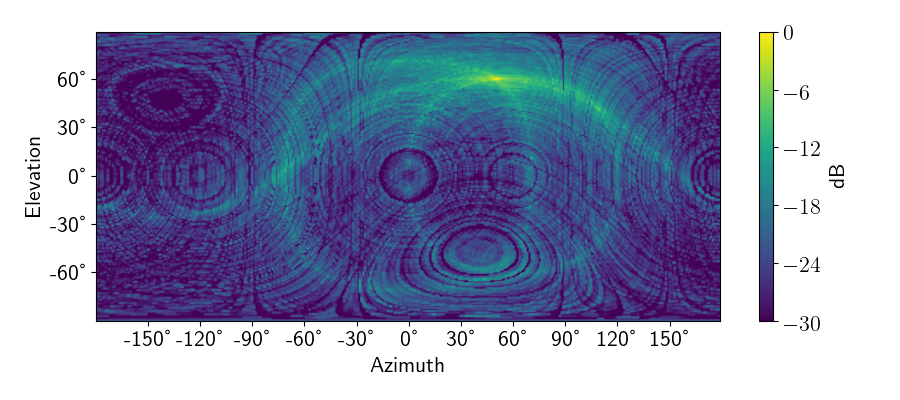
\includegraphics[width=0.8\textwidth]{Figures/Ind4mic1srcProdNeg6.png}
\end{subfigure}
\caption{Figures depict from top-to-bottom product-SRP-PHAT localization results  with SNR = 20dB, SNR = 0dB, SNR = -6dB}
\label{fig:4mic1srcNoisyProd}
\end{figure}
\newpage
The drawback of using product-SRP-PHAT is that the sound level difference between the different sound sources is lost. In normal SRP-PHAT, the array magnitude response at a particular azimuth and elevation is averaged over all microphone pair combinations. Then the level difference between 2 sources is maintained. In product-SRP-PHAT this would not be the case. However if it is assumed that a particular source will have similar magnitude response for all microphone pairs (which is not a strong assumption in far-field), then taking source power $P_{SRP}={S_{SRP}}^{1/M}$, the level difference can be maintained.  Fig. \ref{fig:4mic2srcNoisyCompare} depicts the results of product-SRP-PHAT after level correction.
\begin{figure}[H]
    \centering
    \begin{subfigure}[b]{0.96\textwidth}
    \centering
    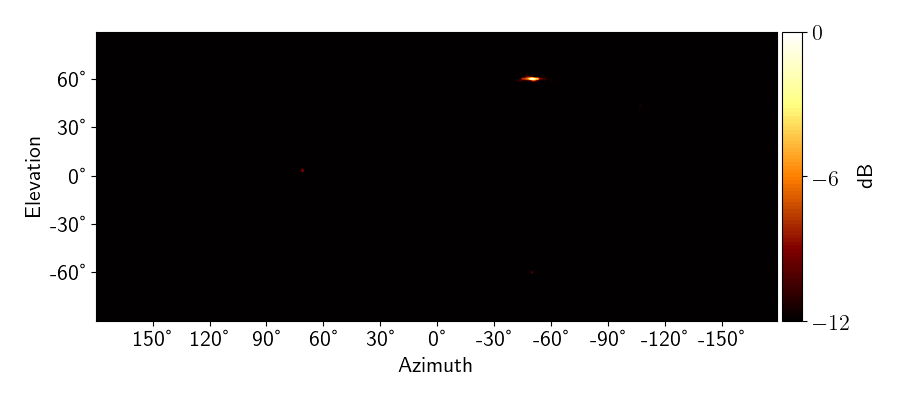
\includegraphics[width=0.8\textwidth]{Figures/Ind4mic1srcProd20Corr.png}
\end{subfigure}
\vskip \baselineskip
\begin{subfigure}[b]{0.96\textwidth}
    \centering
    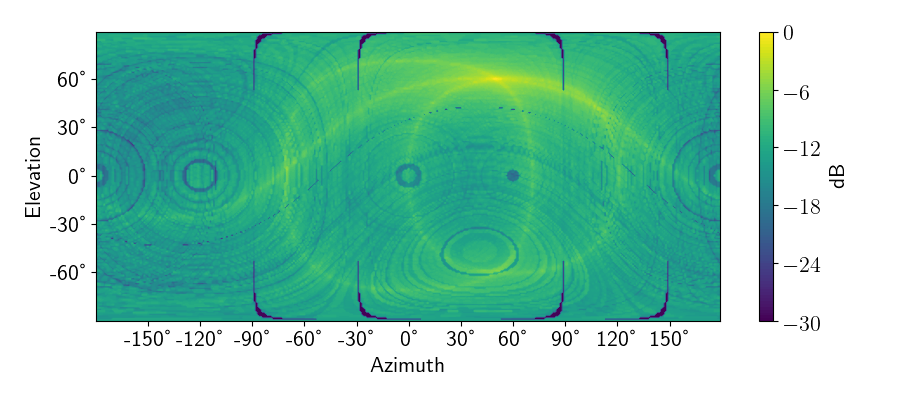
\includegraphics[width=0.8\textwidth]{Figures/Ind4mic1srcProd0Corr.png}
\end{subfigure}
\vskip \baselineskip
\begin{subfigure}[b]{0.96\textwidth}
    \centering
    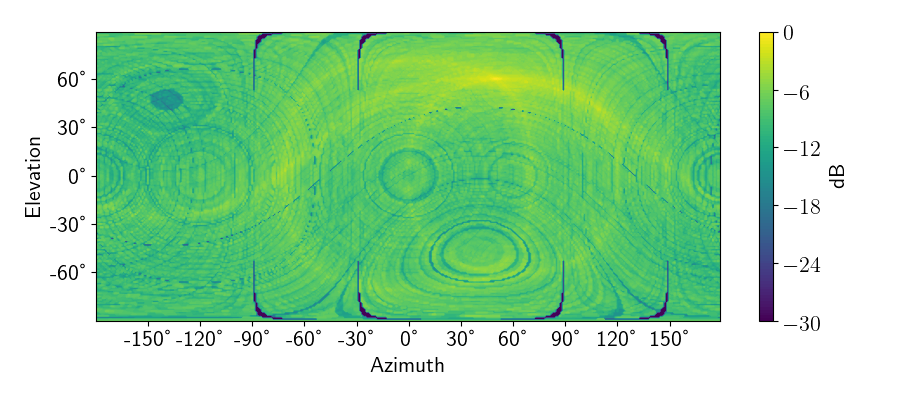
\includegraphics[width=0.8\textwidth]{Figures//Ind4mic1srcProdNeg6Corr.png}
\end{subfigure}
\caption{Figures depict from top-to-bottom level corrected product-SRP-PHAT localization results with SNR = 20dB, SNR = 0dB, SNR = -6dB}
\label{fig:4mic2srcNoisyCompare}
\end{figure}
\subsubsection{Minimum power SRP-PHAT}
Another deconvolution approach can be to use the far-field assumption again, to assume that the power received from a single source to all microphone pairs is the same. In that case, if, the minimum power between the microphone pair is assumed to be the true power (instead of summing), peaks which are detected only by a subset of microphone arrays would disappear automatically and the deconvolution problem can be solved directly. Fig. \ref{fig:4mic1srcNoisyMinPow} shows the results. Even in adverse conditions of -6 dB, the algorithm is fairly able to detect the source at $(50\degree, 60\degree)$. 
\begin{figure}[H]
    \centering
    \begin{subfigure}[b]{0.96\textwidth}
    \centering
    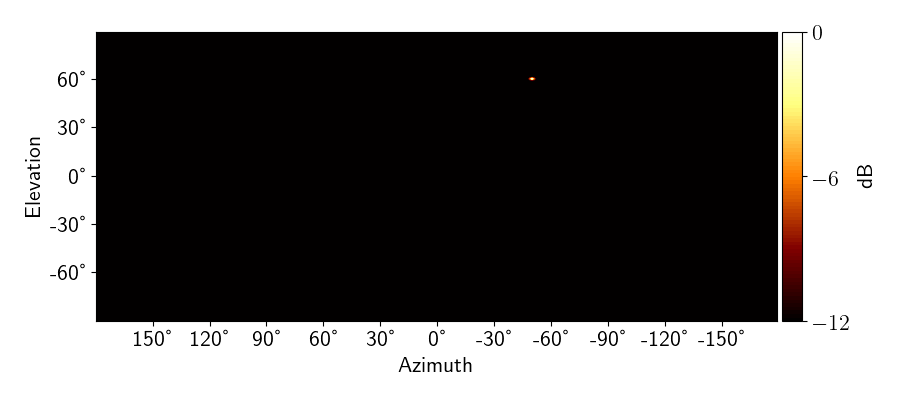
\includegraphics[width=0.8\textwidth]{Figures/Ind4mic1srcMin20.png}
\end{subfigure}
\vskip \baselineskip
\begin{subfigure}[b]{0.96\textwidth}
    \centering
    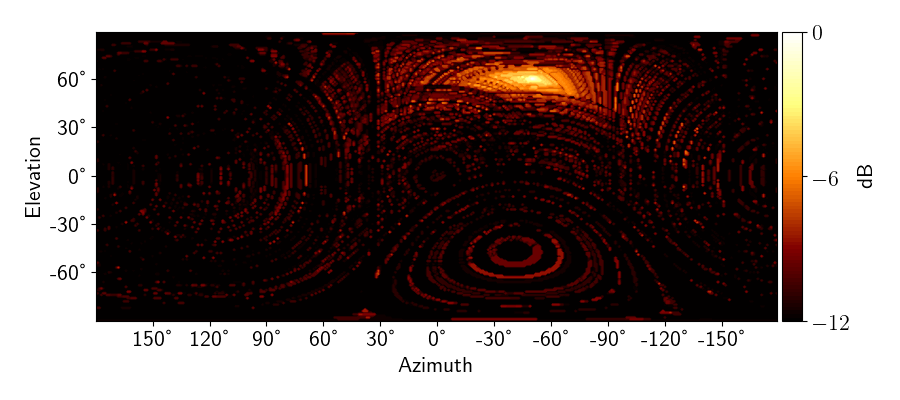
\includegraphics[width=0.8\textwidth]{Figures/Ind4mic1srcMin0.png}
\end{subfigure}
\vskip \baselineskip
\begin{subfigure}[b]{0.96\textwidth}
    \centering
    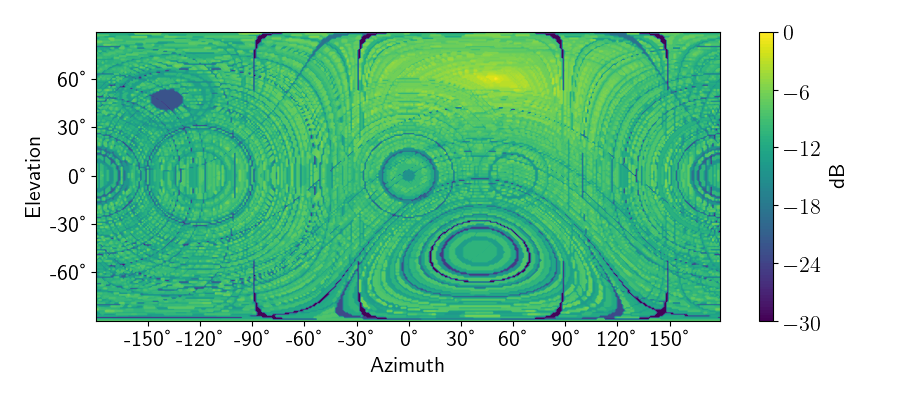
\includegraphics[width=0.8\textwidth]{Figures/Ind4mic1srcMinNeg6.png}
\end{subfigure}
\caption{Figures depict from top-to-bottom minimum power SRP-PHAT localization results with SNR = 20dB, SNR = 0dB, SNR = -6dB}
\label{fig:4mic1srcNoisyMinPow}
\end{figure}
The drawback of both product-SRP-PHAT and Minimum power SRP-PHAT is that in case of localizing point sources, even a minor error in temperature or wind recordings has the potential of not detecting the sound source completely. In real life however, the source is rarely a point source.

\subsection{Other Deconvolution methods}
CLEAN is an algorithm proposed by Jan Högbom in 1974 \cite{1974A&AS...15..417H} to perform the deconvolution of images in radio astronomy. Högbom observed the sky images being polluted by what he described as the "dirty beam". This "dirty beam" is the distortion introduced in the system output when the input is subject to a point source. It relates to the point spread function (PSF) in optic or the array response in our case. The CLEAN algorithm removes the side lobes of the beamformer when the PSF is known in advance throught simulation or measurement. CLEAN-SC is an extension of the CLEAN algorithm but does not rely on knowing the PSF in advance, it uses the coherence between the sidelobes and the main beam to identify the PSF and retrieve the level of the sources. Usually efficient deconvolution is performed in the frequency domain when the PSF is shift-invariant but in our case the PSF change for every scanned position as the array response is different therefore it can become challenging to perform the deconvolution on a real time system. The CLEAN and CLEAN-SC algorithm and some notation will be introduced as well as the algorithm issues. Methods to overcome those issues are also discussed.

\subsubsection{CLEAN deconvolution of the beamformed maps}

The energy map obtained with the SRP-PHAT algorithm is composed of N sound sources of complex amplitude $\hat{A_{N}}$ convoluted with the array response $p(t)$ and some noise n(t). This "image" I(t) can be expressed as in equation \ref{eq:imageclean}
\begin{equation}
    I(t)=\sum\limits_{n=1}^{N}{A_{n}p(t-t_{n})+n(t)}
    \label{eq:imageclean}
\end{equation}

In real situation it might be difficult to retrieve the sources information in this noisy map. A naive and straightforward solution consist in subtracting the array response of the strongest peak and so on until there is no prominent peak left on the map. By subtracting the array response (PSF), a residual image $I_{m}$ is created.

\begin{equation}
    I_{m}(t)=I(t)-\hat{A}_{m}p(t-\hat{t}_{m})
\end{equation}

This idea is among the line of the CLEAN algorithm where usually a fraction of the PSF is deconvoluted from the map. However this method has several drawbacks such as assuming the main peak to be a source and not an addition of interferences created by other sources. Also it assumes the number of sources to be known in advance. To overcome this problem and retrieve the real sources among interferences, a PSF correlation algorithm has been described in \cite{freedman1995techniques}. The PSF Correlation algorithm define the minimal target mass criterion as follow:

\subsubsection{The PSF correlation algorithm}

    \begin{equation}
        M_{m}=\int_{-\infty}^{\infty}|{(I_{m}(t))}|^2
    \end{equation}
    
    \begin{equation}
        \begin{split}
        M_{m} & =\int_{-\infty}^{\infty}\{{(I(t)-\hat{A}_{m}p(t-\hat{t}_{m})}\}\{{(I(t)-\hat{A}_{m}p(t-\hat{t}_{m})}\}^*dt \\
              & = M + |{\hat{A}_{m}}|^2M_{p}-2Re[{\hat{A}_{m}}{R^*_{pl}(\hat{t}_{m})}]\\
              & = M + |{\hat{A}_{m}}|^2M_{p}-2|{\hat{A}_{m}}||{R_{pl}(\hat{t}_{m})}|cos(\hat{\alpha}_{m}-\phi(\hat{t}_{m})
        \end{split}
    \end{equation}

$M_{p}$ is the mass of the point spread function and $R_{pl}(\hat{t_{m}})=\int_{-\infty}^{\infty}{p^{*}(t-\hat(t_{m})I(i)dt}$ is the cross-correlation function between the image and the PSF.
The intuition of the PSF correlation algorithm is that there exists an optimal position $\hat{t}$ which minimize this criteria. This optimal target position to cancel can then be inputed in the CLEAN Algorithm itself.\\

\subsubsection{CLEAN-SC deconvolution of the beamformed maps}

The CLEAN method is attractive in simulation as the cones intersect in one point but as explained earlier it will never happen in practice, there will never be clean cone intersections in the beamformed results due to microphone error position, speed of source shift or wind effect. It is therefore challenging to know what PSF to substract from the map since there is no clean peak in the map. CLEAN-SC is an addition to the CLEAN methods but no assumption about the PSF is made and the PSF is retrieved using the coherence information between the main lobes and the side lobes. The algorithm also retrieves the sources amplitudes, it is interesting to note that the computation time of the CLEAN-SC is usually twice the one to compute the beamformed map, as stated earlier no real time implementation is considered but it is nevertheless interesting to note. CLEAN-SC \cite{sijtsma2007clean} has been published in 2007 by Pieter Sijtsma and the algorithm basics will be explained in this section. Let's first define the Cross Spectrum Matrix (CSM) $\hat{C}$ given by
\begin{equation}
\hat{C}=
    \begin{bmatrix} 
      C_{11} & C_{12} & \cdots & C_{1m_{0}}\\
      \vdots &  C_{22} &       &  \vdots\\
      \vdots &         & \ddots &  \vdots\\
      C_{m_{0}1} &     &       &  C_{m_{0}m_{0}}\\
    \end{bmatrix}  
\end{equation}
where $C_{mm'}$ is the cross spectrum between microphone m  and m'. It is computed by taking the FFT of the pressure recording $p^{*}_{mk}(t)$ and $p_{m'k}(t)$ averaged over K data blocks. $w_{s}$ is a weight filter like Hamming window.
\begin{equation}
    C_{mm'}=\frac{2}{Kw_{s}T}\sum\limits_{k=0}^{K}[P^{*}_{mk}(f,T)P_{m'k}(f,T)]
\end{equation}

Usually a trimmed CSM is used in order to only get the information of independent pairs of microphones, ie all the possible (m,n) combinations of microphones forming the subset S, with m and n the microphones indices. The trimmed CSM  ${\xoverline{C}_{mn}}$ is defined in equation \ref{eq:trimmedcsm}

\begin{equation}
     \xoverline{C} = 
      \begin{cases} 
       C_{mn} & \text{for } (m,n) \in S \\
       0      & \text{for } (m,n) \notin  S
      \end{cases}
    \label{eq:trimmedcsm}
\end{equation}

Let's now define the degraded CSM  $D^{i}$ when source components are removed and the CSM induced by peak source steering vector , $G^{i}$. The indice i is due to the process being iterative as sources are removed from the map. The source cross powers $B_{jk}$ is defined by the equation \ref{eq:crosspow} 

\begin{equation}
    B_{jk}=w_{j}^{*}\xoverline{C}w_{k}
    \label{eq:crosspow}
\end{equation}

with w, the weight vector defined from the steering vector as in equation \ref{eq:weightcsm}

\begin{equation}
    w=g/\sum\limits_{m,n\in S}(|{(g_{m})}|^2|{(g_{n})}|^2)^{1/2}
    \label{eq:weightcsm}
\end{equation}

The CLEAN-SC algorithm demands the source cross-powers of any scan point to be determined entirely by $G^{i}$.

\begin{equation}
    w_{j}^{*}{\xoverline{D}}^{i-1}w^{i}_{k}=w_{j}^{*}\xoverline{G}^{i}w^{i}_{k} 
\end{equation}

This equation has several solution but we can assume the $G^{i}$ to due to a single coherent source component $h^{(i)}$. 

\begin{equation}
    G^{i}=P_{max}^{(i-1)}h^{i}h^{*(i)}
\end{equation}



\subsection{The MP-SRP-PHAT algorithm}

The MP-SRP-PHAT implementation steps are described in Fig. \ref{fig:systemimplementaiton}. The algorithm is basically the same as the normal SRP-PHAT algorithm discussed before, with the only change happening at the last step where the minimum power from the localization cones is considered, instead of summing the power from all the cones.  % there exist methods to improve the efficiency of the algorithm but this is not the focus of this work. \footnote{Dmochowski and Benesty \cite{dmochowski2007generalized} present a method which improve the full map search}. 
The computational complexity of the algorithm and the practical implementation details are discussed in this section. The delays across the microphones for each search location on the search map are computed in advance, stored in memory and fed to the algorithm which correspond to the `Compute array delays' system block in the figure, therefore this step will not be considered computational load. Upon running the algorithm, first of all the computer reads the stored .wav files into memory. The signal cross correlation between each pair of microphones are then computed. This step is the `GCC-PHAT' block in Fig. \ref{fig:systemimplementaiton}. The `SRP' system block is related to the array steering for each of the search location $(\theta,\phi)$. This step looks up the delay table corresponding the $(\theta,\phi)$ for each microphone pair, and saves the corresponding power associated with that delay and that pair into an array ($P_{all}$). So $P_{all}$ contains 6 power values for each location on the search map. The minimum power then selected from $P_{all}$ the 6 power values for each of the locations $(\theta,\phi)$ and this value is stored in the result array\footnote{One thing to note is that there is a limit to the granularity of the $(\theta,\phi)$, the achievable angular resolution. The angular resolution of localization is in fact not linear, as shown in \ref{fig:ang_res}(A delay of one sample does not always correspond to the same change in degree). The SRP-MAP can then be plotted by computing the delays sequentially for a particular angular resolution. However, these delays might be fractional. Since, the values of fractional delays cannot be picked from the cross-correlation array \textit{R}, these delays are rounded. One way to increase the angular resolution is to increase the sample rate. That way even if fractional delays are encountered, they would be less erroneous. Another way is to apply interpolation to find the value at the fractional delays. For the purpose of this thesis, the interpolation techniques are not considered.}.

\begin{figure}[!ht]
    \centering
    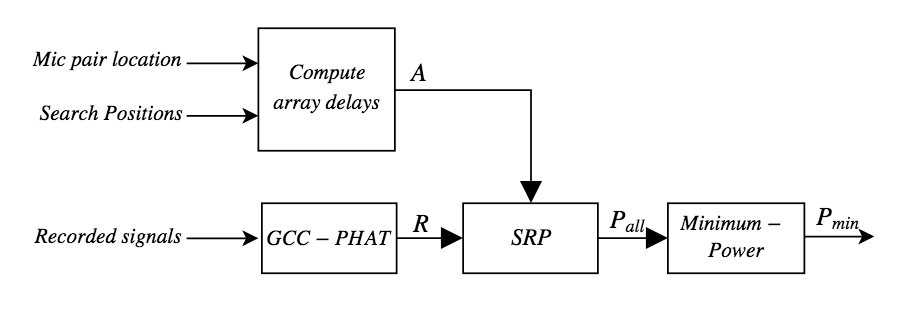
\includegraphics[width=1\textwidth]{Figures/system1.png}
    \caption{Overall localization algorithm}
    \label{fig:systemimplementaiton}
\end{figure}

The MP-SRP-PHAT algorithm combines beamforming techniques with cross correlation methods for several pairs of microphones. While the beamforming part does not depend on the size of the input data, it might become a challenge memory wise to store the delay for each search position. The most computationally demanding part of the algorithm is definitely the cross-correlation part. By performing the cross-correlation in the frequency domain, i.e by using the cross-spectrum between pairs of microphones, better averaging of the stationary sources are obtained as well as better efficiency compared to time domain cross-correlation ($\mathcal{O}(n^2)$). The cross-spectrum computation is described in Fig. \ref{fig:crossspectrumsystem}.
\begin{figure}[H]
    \centering
    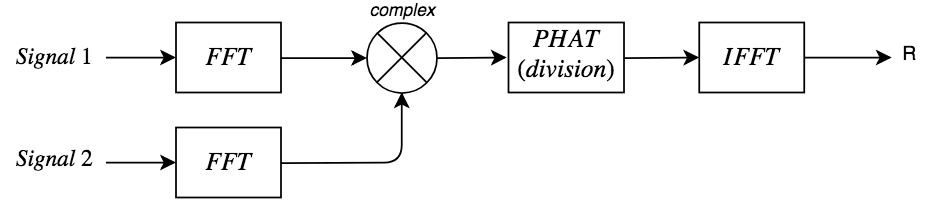
\includegraphics[width=1\textwidth]{Figures/crossspectra.png}
    \caption{Cross spectrum between two signals}
    \label{fig:crossspectrumsystem}
\end{figure}
%Dmochowski and Benesty \cite{dmochowski2007generalized} detailed the number of computation needed for the GCC-PHAT part,
Note that not the entire R computed this way is important for the purpose of localization. This is because only a finite number of samples can exist between two microphones, say \textit{d}. \textit{d} depends on the array aperture size as well as the sample rate. Delays$\gt$\textit{d} could not have been measured by the microphone array. For this reason the R is cropped down to \textit{d}. Since, the signals arriving at two microphones can be either in front or behind each other, both the first and last \textit{d} samples of R are taken. The worst-case complexity of the cross-spectrum computation is listed below, with \textit{n} being the number of input samples (signal length) in the algorithm. 
\begin{center}
  \begin{tabular}{ |c | c | }
    \hline
    Operation  & Worst-case Complexity \\ \hline
    FFT  & $\mathcal{O}(n\log{}n)$  \\ \hline
    Complex Multiplication  & $\mathcal{O}(n)$  \\ \hline
    PHAT (Division)  & $\mathcal{O}(n)$  \\ \hline
    IFFT  & $\mathcal{O}(n\log{}n)$  \\
    \hline
  \end{tabular}
\end{center}
The SRP block is also computationally heavy, however, it does not scale with the number of samples but rather with the number of locations to look up in the SRP block. %Dmochowski and Benesty \cite{dmochowski2007generalized} also proposed a more efficient way to perform the SRP.
Therefore the overall algorithm complexity scales with the FFT complexity $\mathcal{O}(n\log{}n)$ when n is the number of samples. %When n is small the FFT is negligible to the number of delay lookups.
\begin{figure}[!ht]
    \centering
    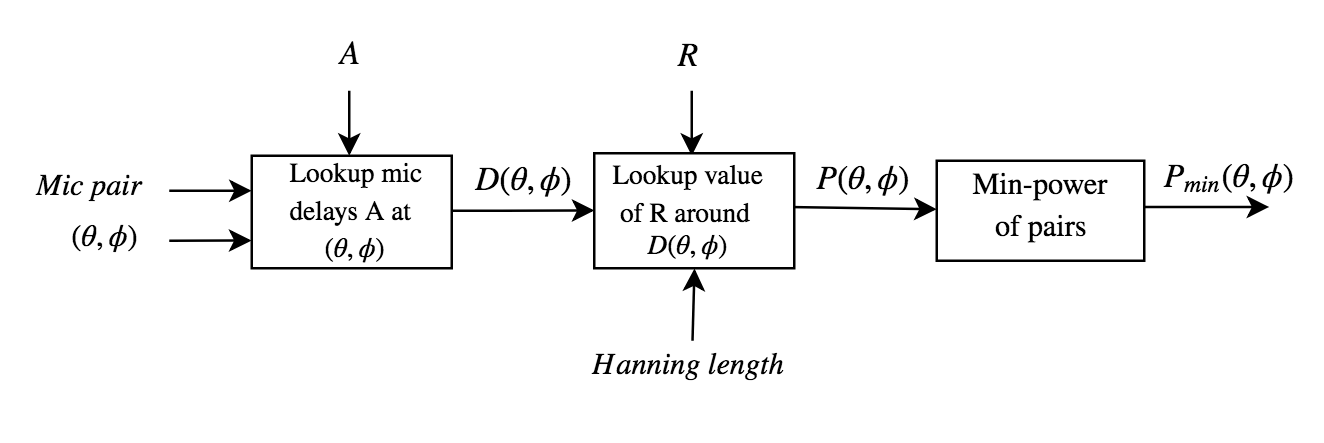
\includegraphics[width=1\textwidth]{Figures/system2.png}
    \caption{SRP block + Minimum Power}
    \label{fig:system2}
\end{figure}
%Table \ref{tab:extime} gives a measure of the execution time of the minimum SRP-PHAT script. 
%\begin{center}
%  \begin{tabular}{ c | c | c |}
%    \cline{2-3}
%    \multicolumn{1}{c|}{} & \multicolumn{2}{ c| }{Execution time} \\ \cline{2-3}
%    \hline
%    \multicolumn{1}{|c|}{signal lengths (seconds)}   & thinkpad i5 & Macbook 2012  \\ \cline{1-3}
%    \multicolumn{1}{|c|}{10}  &  &    \\ \cline{1-3}
%    \multicolumn{1}{|c|}{100} & &     \\ \cline{1-3}
%    \multicolumn{1}{|c|}{1000}  & &   \\
%    \hline
%  \end{tabular}
%  \label{tab:extime}
%\end{center}
Memory wise, the function computing the delays at each pair of microphones in the array can be expensive depending on the localization resolution used and the number of microphone pairs. If 1$\degree$ resolution is used $360*180=64800$ delays are computed for a pair of microphones. For 6 microphone pairs,$360*180*6=388800$.  Using type float64 (8 bytes), the delay table is  $360*180*6*8=3110400$ = 3.11 MB. However, if high resolution is needed, i.e suppose 0.1$\degree$ resolution $3600*1800=6480000$ delays are computed. For 6 microphones,$3600*1800*6=38880000$.  Using type float64 (8 bit), the delay table is  $3600*1800*6*8=311040000$ = 311.04 MB.
\section{Normal SRP-PHAT vs MP-SRP-PHAT}
Comparison between the performance of normal SRP-PHAT vs MP-SRP-PHAT are done in this section. Simulations are provided to outline the robustness of the normal SRP-PHAT vs the MP-SRP-PHAT for various environmental aspects and sound source conditions. Effects of practical considerations such as the choice of array aperture size the recording sample rate, and the length of recording are shown. Finally, the robustness of the algorithms for errors in the microphone array placement are given.
\subsection{Effect of outdoor environment}
When localizing sound sources, the propagation environment can affect the signals received at the microphones. For outdoor environments, understanding the localization results thus requires knowledge of the physical phenomena at play at the time of the measurement\footnote{For more information on the theory behind outdoor sound propagation are refer Appendix \ref{app_outdoor}}. The effect of ground reflections, temperature and wind are provided here.
\subsubsection{Effect of ground reflections}
\begin{figure}[!ht]
\centering
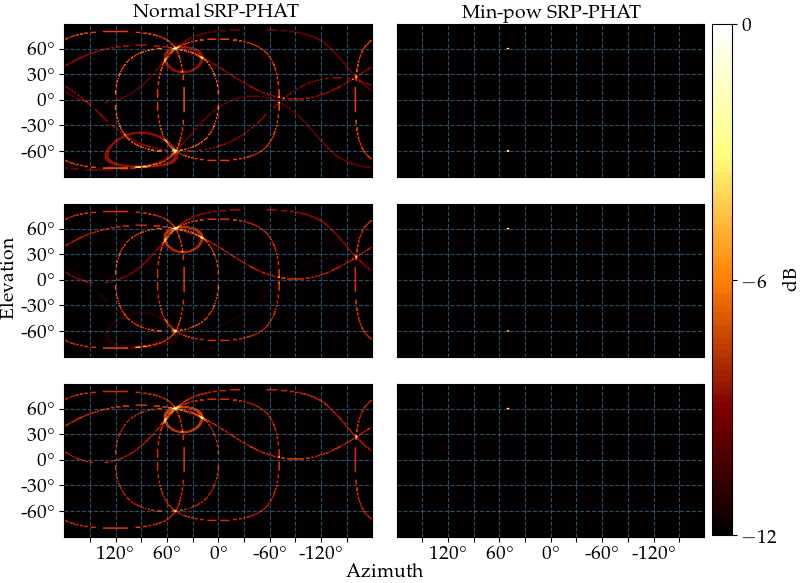
\includegraphics[width=\textwidth]{Figures/refSim.png}
\caption{Figures depict from top-to-bottom SRP-PHAT localization results for a source at ($50\degree$,$60\degree$) with ground reflection coefficients (R) of 1, 0.6 and 0.1. For normal SRP-PHAT, even though the image source should get significantly weaker for R=0.1, it does not as it is supported by the localization cones from the real source. MP-SRP-PHAT, however, is able to detect the source and the image powers correctly.}
\label{fig:4mic1srcRef}
\end{figure}
Sound received from a far-field sound source is the sum of a plane and a spherical wave component (Eq. \ref{Eq:GroundWave}). The spherical wave component creates a horizontal ground wave and quickly attenuates with distance. The plane wave component is reflected with the ground (image source), the magnitude of the reflection depends on the acoustic reflection coefficient of the ground material. Rudimentary simulations for a source located at $(\theta,\phi)$ can be made assuming image sound source located at $(\theta,-\phi)$. Fig. \ref{fig:4mic1srcRef} shows the localization results with a source at ($50\degree$,$60\degree$) for different ground reflection coefficients. The microphone pairs in the tetrahedral array that are parallel to the ground (horizontal) locate both the source and the image on the same cone. If the array is then placed such that three of its microphones are on the same horizontal plane, three out of the six possible cones will be shared. For normal SRP-PHAT, this causes the image to be localized at a higher level than it actually is\footnote{One way to mitigate this issue would be to not place the array horizontally, the simulations for this are given in Appendix \ref{sec:refTilted}}. 
\subsubsection{Effect of temperature}
\begin{figure}[!ht]
\centering
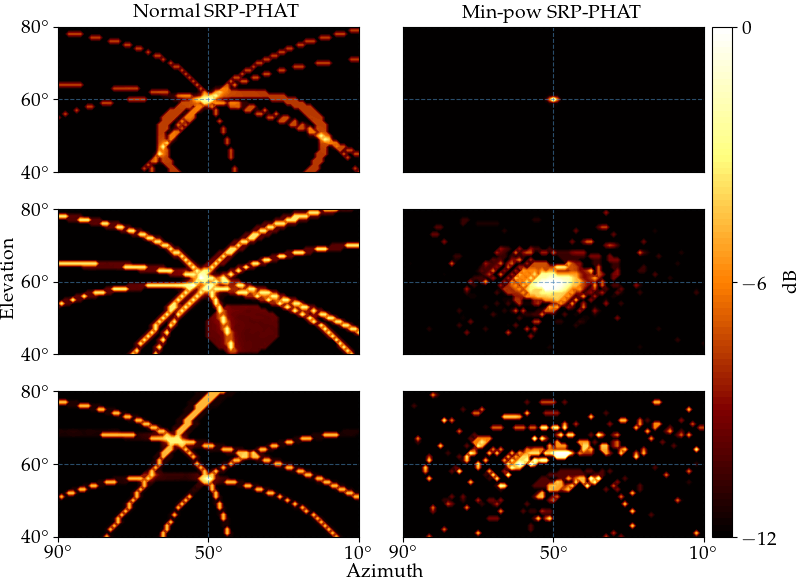
\includegraphics[width=\textwidth]{Figures/tempSim.png}
\caption{Figures depict from top-to-bottom SRP-PHAT localization results for a source at ($50\degree$,$60\degree$) with at temperatures of $20\degree C$, $0\degree C$ and $-40\degree C$. The extreme temperature of $-40\degree C$ is chosen to highlight the error.} 
\label{fig:4mic1srcTemp}
\end{figure}
Temperature affects the speed of sound and thus affects the delay time between the microphone pairs. During measurement, if the speed of sound is assumed to be 343m/sec, this could lead to errors in the localization results. Fig. \ref{fig:4mic1srcTemp} depicts the effect of temperature on localization results for a source at ($50\degree$,$60\degree$) , where wave files received by the tetrahedral microphone array at temperatures of $0\degree C$, $20\degree C$ and $-40\degree C$ are simulated. Then the localization is run assuming the speed of sound to be 343m/sec in every case. The figure shows zoomed in results around the source location. As can be seen in the figure, if temperature is not considered, it has the effect `de-focusing' the main peak. If temperature is recorded during measurements, the localization can be run using the correct speed of sound, which would remove this de-focusing issue\footnote{Since, the speed of sound is greater at higher temperatures, the number of samples that can fit within the array aperture would reduce. This can also have an effect on the localization results, however, this error is relatively minor. The effect of sample rates on localization results have been discussed later.}. For this reason, the temperature is recorded whenever outdoor measurements are done. 
\subsubsection{Effect of wind}
\begin{figure}[H]
\centering
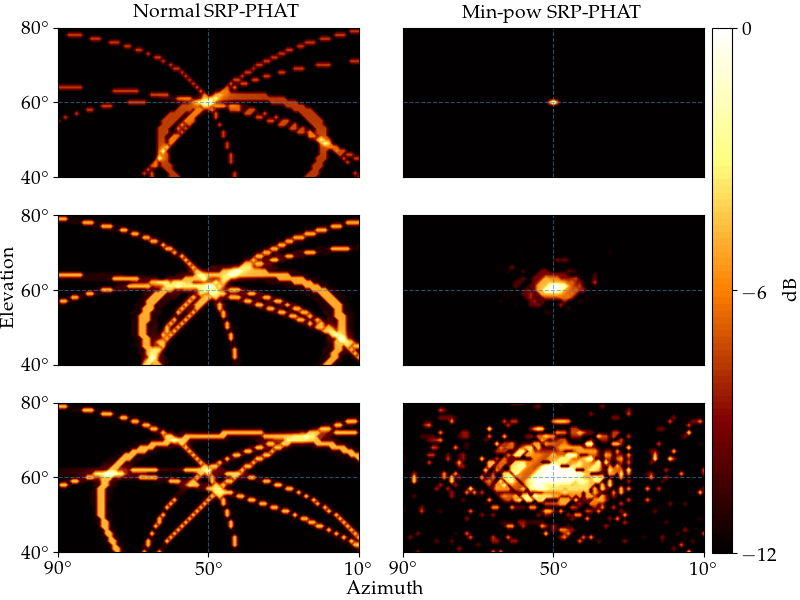
\includegraphics[width=\textwidth]{Figures/windSim.png}
\caption{Figures depict from top-to-bottom SRP-PHAT localization results with wind of $10 m/sec$ blowing $90\degree$, $10 m/sec$ blowing $45\degree$ and $30 m/sec$ blowing $45\degree$ to the source sound propagation direction. The extreme wind of $30 m/sec$ is chosen to highlight the error.}
\label{fig:4mic2srcWind}
\end{figure}
Wind speed effects the speed of sound in the direction of propagation. However unlike temperature, which causes a uniform difference in delays across the different microphone pairs, wind causes the delays to be affected differently depending on where the SRP search is looking and from what direction the wind is blowing. If wind blows perpendicular to the direction of propagation of the sound from the source, then it does not affect the localization. The maximum error happens exactly in and against the direction of the wind. Fig.\ref{fig:4mic2srcWind} depicts the effect of wind on localization results at wind of 10$m/s$ blowing at $90\degree$, $45\degree$ and $180\degree$ to the direction of propagation of sounds from a source at ($50\degree$,$60\degree$). It can be seen that when wind blows at $90\degree$, it does not affect the localization results. The magnitude of error when wind blows non-perpendicular to the sound propagation direction depends on the wind speed and the degree of alignment with the wind direction. For normal SRP-PHAT, an error in wind causes the localization cones to not overlap perfectly. For MP-SRP-PHAT, this causes a lowering of the peaks. This is because the localization circles are annular with peaks in the middle of the annular ring (a 3D torus). A movement in the tori causes the overlap to not happen perfectly, lowering the peaks. This error can be corrected during the SRP search, if the wind is recorded at the time of measurements. However, when doing outdoor measurements, the wind was rarely from a uniform direction. For this reason, the outdoor measurements were only done in relatively low wind conditions (<5m/sec), and no wind correction was applied.
\subsection{Effect of source conditions}
An extremely wide variety of outdoor sound sources exist. They can be spread-out or point sources, narrow-band or wide-band, be uniform across the frequency spectra, or have a lot of low frequency or high frequency content, moving or stationary, constant or transient. To keep the simulations within scope, some outdoor measurements were conducted to realize the major factors that can affect the localization. Based on those measurements, the effect of sound source SNR and the effect of coherence between multiple sound sources were selected. The simulations for those effects are given in this section.
\subsubsection{Effect of SNR}
\begin{figure}[H]
\centering
%\hspace*{-1cm}
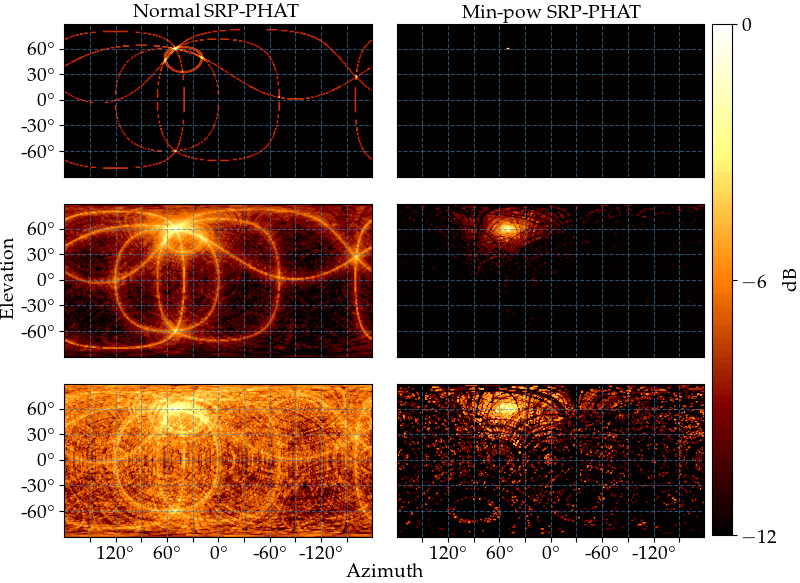
\includegraphics[width=\textwidth]{Figures/noiseSim.png}
\caption{Figures depict from top-to-bottom localization results with SNR = 20dB, SNR = 0dB, SNR = -6dB}
\label{fig:4mic1srcNoisy}
\end{figure}
The source SNR and overall magnitude is an important factor for localizing a source. Even if a source has a high sound level, if the SNR is low, the localization results might be poor. The error due to SNR has been discussed before for GCC comparison for a single pair of microphones, shown in Fig. \ref{fig:GCC_SIM}, where white noise is used for the simulations and it caused an almost uniform increase of the noise floor across all locations for GCC-PHAT. The same happens for tetrahedral localization, wherein, the noise floor across the entire noise map rises with falling SNR. Fig. \ref{fig:4mic1srcNoisy} shows the effect of source SNR on localization, with a point source at ($50\degree$, $60\degree$). As can be seen in the figure, the performance deteriorates as the SNR drops. However, understandably, the noise floor is lower for MP-SRP-PHAT, as it clears some of the noise results where not all cones overlap.
%\subsubsection{Minimum power SRP-PHAT}
\subsubsection{Effect of coherent sound sources}\label{sec:Coherent}\begin{figure}[H]
\centering
%\hspace*{-1cm}
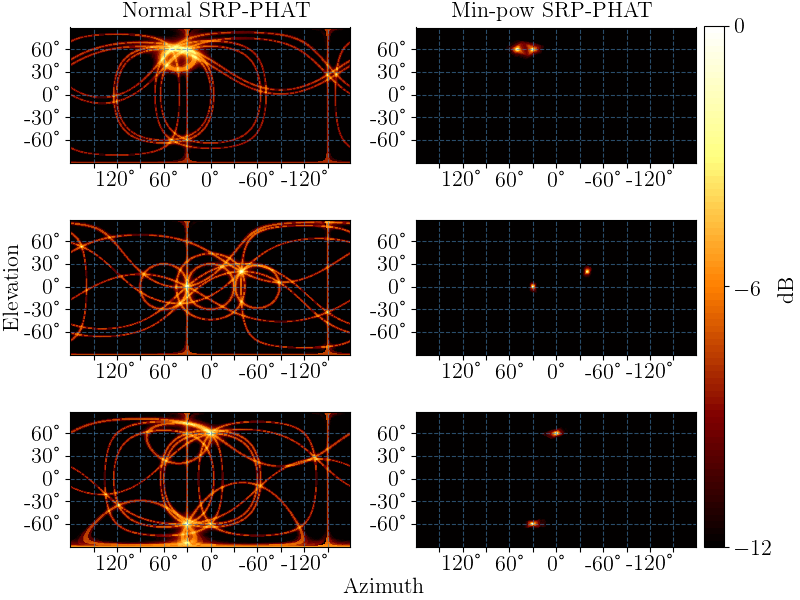
\includegraphics[width=\textwidth]{Figures/simCoherenceFalse.png}
\caption{Figures depict from top-to-bottom localization results for two sources located at ($50\degree$,$60\degree$) and ($30\degree$, $60\degree$), at ($40\degree$, $20\degree$) and ($30\degree$, $0\degree$), and at ($0\degree$, $60\degree$) and ($30\degree$, -$60\degree$) respectively. The sources are playing uncorrelated pink noise and the SNR is 6dB.}
\label{fig:4mic1srcCoherenceFalse}
\end{figure}
Fig. \ref{fig:4mic1srcCoherenceFalse} shows the localization results for two sound sources playing uncorrelated pink noise from different locations. As can be seen, both normal SRP-PHAT and MP-SRP-PHAT detect the peaks of the source correctly in all the cases. However, if multiple sound sources at different locations play coherently, i.e., the same waveform having a constant phase difference between each other, there is a possibility to detect a pseudo-source corresponding to the phase difference between the sound sources. This is because GCC algorithms inherently depend on the phase difference between the receiving waveforms to do the localization\footnote{The same error happens with human ears which causes detection of a stereo image in a 2 channel loudspeaker setup. Changing the inter-aural time difference causes this phantom image location to shift as well.}. The localization result for when 2 sources play the same pink noise are depicted in fig. \ref{fig:4mic1srcCoherence}. As can be seen in the figure, coherence has an effect on the localization, wherein, pseudo-peaks appear around the main sound source. The magnitude of these pseudo-peaks depends on their proximity and the phase difference. The effect of coherence is also seen later in an outdoor measurement, where multiple loudspeakers were playing music in an outdoor environment.
\begin{figure}[H]
\centering
%\hspace*{-1cm}
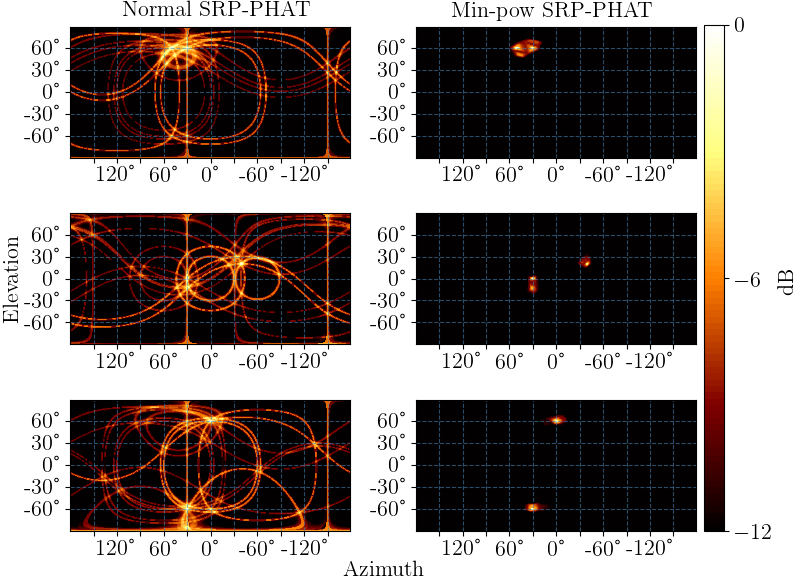
\includegraphics[width=\textwidth]{Figures/simCoherenceTrue.png}
\caption{Figures depict the localization results for when the sources from the previous figure play coherently. The sources here play the same pink noise. Pseudo-peaks can be seen to appear around the main sound sources.}
\label{fig:4mic1srcCoherence}
\end{figure}



\section{Practical measurement considerations}
Some practical measurement considerations can have a considerable effect on the localization results. For instance, the delay table that is computed for the SRP-MAP has a maximum magnitude, \textit{d}. This is because the microphone array can measure signal delays only within a finite value. Thus, \textit{d} is the number of samples that can fit within two microphones of the array. Obviously, \textit{d} depends on the array aperture and also the sample rate of recording. Higher \textit{d} values are preferable as that directly translates to a higher achievable resolution on the SRP-MAP (\ref{app:angRes}).
\subsubsection{Effect of array aperture and sample rate}
As discussed above and shown in Fig. \ref{fig:res_diff}, reducing the aperture size or sample rate also reduces the angular resolution of localization, which causes a direct degradation in SRP-PHAT performance. Fig. \ref{fig:4mic1srcAper} depicts the effect of reducing sample rate or aperture size on the SRP-PHAT localization results. Any reduction in the array aperture of the sample rate causes the localization circles to become annular. This is because more $\theta$s and $\phi$s correspond to the same integral delay. These issues can be somewhat alleviated if the algorithm considered fractional delays and interpolation. However, even with interpolation, some data between the integral delays is always lost. For the outdoor localization, a sample rate of 131072Hz is used, which results in an angular resolution of 
\begin{figure}[H]
    \centering
    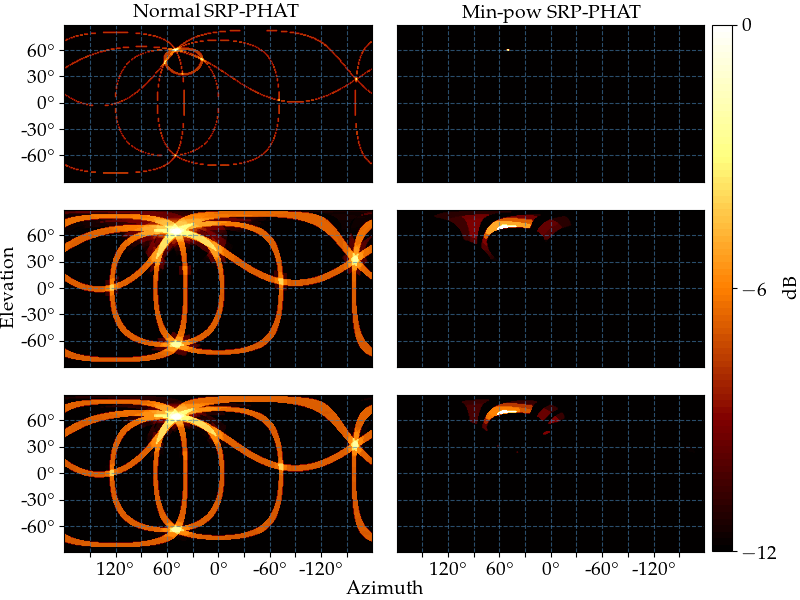
\includegraphics[width=\textwidth]{Figures/aperSampSim.png}
    \caption{Figures depict from top-to-bottom SRP-PHAT localization results with tetrahedral microphone array aperture size of 1m@48kHz, 10cm@48khz and 1m@4.8kHz.}
    \label{fig:4mic1srcAper}
\end{figure}
\subsubsection{Effect of audio recording length}
\begin{figure}[H]
    \centering
    \includegraphics[width=\textwidth]{Figures/audioLenSim.png}
    \caption{Figures depict from top-to-bottom SRP-PHAT localization results with tetrahedral microphone array with recording length of 1sec  (top), 10sec (middle) and 100sec (bottom)}
    \label{fig:micErrTilt}
\end{figure}
%\subsubsection{Effect of adding more microphones}
%It is of interest to test the scalability of the algorithm by adding more microphones. Theoretically, adding microphones should add independent pairs and thus lower the noise floor (normalized) to improve results in a low SNR scenario. 
%\begin{figure}[H]
%\begin{subfigure}[b]{0.96\textwidth}
%    \centering
%    \includegraphics[width=0.8\textwidth]{Figures/Ind4mic1srcResNeg10LowDyn.png}
%\end{subfigure}
%\vskip \baselineskip
%\begin{subfigure}[b]{0.96\textwidth}
%    \centering
%    \includegraphics[width=0.8\textwidth]{Figures/Dep4mic1srcResNeg10LowDyn.png}
%\end{subfigure}
%\caption{Figures depict from SRP-PHAT localization results with SNR = -10dB, for independent microphone pairs (top), and for all  microphone pairs (bottom)}
%\label{fig:4mic1srcRedun}
%\end{figure}
\
\subsubsection{Effect of error in mic position}
The microphones in the array could have an error in position, due to structural errors (structural fatigue and sag, thermal expansion/ contraction or just human error). This could lead to an error in localization. Fig. \ref{fig:micErrPos} illustrates this effect. 
\begin{figure}[H]
    \centering
    \includegraphics[width=\textwidth]{Figures/micErrPosSim.png}
    \caption{Figures depict from top-to-bottom SRP-PHAT localization results with tetrahedral microphone array with no mic error in placement (top), a 1cm placement error in 1 mic (middle), a 2cm placement error in all mics (bottom)}
    \label{fig:micErrPos}
\end{figure}

\subsubsection{Effect of error in array tilt}
\begin{figure}[H]
    \centering
    \includegraphics[width=\textwidth]{Figures/micErrTiltSim.png}
    \caption{Figures depict from top-to-bottom SRP-PHAT localization results with tetrahedral microphone array with no mic tilt error (top), a +10$\degree$ tilt  error (middle) along the x-axis and a -20$\degree$ tilt error along the x-axis (bottom)}
    \label{fig:micErrTilt}
\end{figure}



%\subsection{Deconvolution old part}

\subsubsection{CLEAN}

CLEAN is an algorithm used to remove the influence of the point spread function (PSF) on the beamformed result. It is possible to remove the side lobes of the beamformer and get a more accurate localization, but it requires many microphones. CLEAN-SC is an extension of the algorithm for the case of coherent sources, it performs the deconvolution in the frequency domain which usually assumes a shift-invariant PSF. A deconvolution technique in the time domain was developed named TIDY (add reference).

\subsubsection{DAMAS}

Conventional beamforming produces an output that is dependent on array geometry, size, source distance, and frequency. DAMAS removes those array-dependent beamforming characteristics from the output to give an explicit and non ambiguous source localization and level. The DAMAS use the steering vector $\hat{e}$ of the array defined in section.. and formulates that the output of a standard beamformer with $m_{0}$ microphones can be written as:

\begin{equation}
    Y=\frac{\hat{e}^{T}\hat{G}\hat{e}}{m_0^2}
    \label{eq:DAMASoutputbeamformer}
\end{equation}
where $\hat{G}$ is the Cross Spectral Matrix (CSM) given by
\begin{equation}
\hat{G}=
    \begin{bmatrix} 
      G_{11} & G_{12} & \cdots & G_{1m_{0}}\\
      \vdots &  G_{22} &       &  \vdots\\
      \vdots &         & \ddots &  \vdots\\
      G_{m_{0}1} &     &       &  G_{m_{0}m_{0}}\\
    \end{bmatrix}  
\end{equation}
$G_{mm'}$ is the cross spectrum between microphone m  and m'. It is computed by taking the FFT of the pressure recording $p^{*}_{mk}(t)$ and $p_{m'k}(t)$ averaged over K data blocks. $w_{s}$ is a weight filter like Hamming window.
\begin{equation}
    G_{mm'}=\frac{2}{Kw_{s}T}\sum\limits_{k=0}^{K}[P^{*}_{mk}(f,T)P_{m'k}(f,T)]
\end{equation}

Pressure at the two microphones $p^{*}_{mk}(t)$ and $p_{m'k}(t)$ can be split to form two terms accounting for the amplitude of the signal and the steering vector, such that the cross spectrum for a single source can be written as the product of the squared pressure with the cross spectrum of the steering vectors K:

\begin{equation}
\hat{G}_{n}= X_{n} 
\begin{bmatrix} 
      e_{1}^{-1}^{*}e_{1}^{-1} & e_{1}^{-1}^{*}e_{2}^{-1} & \cdots &   e_{1}^{-1}^{*}e_{m_{0}}^{-1}\\
      e_{2}^{-1}^{*}e_{1}^{-1} & e_{2}^{-1}^{*}e_{2}^{-1} &       &  \vdots\\
         &     & \ddots &   \vdots\\
       &     &   &   e_{m_{0}}^{-1}^{*}e_{m_{0}}^{-1}\\
    \end{bmatrix}_{ n}= X_{n}.K 
\end{equation}   

DAMAS assumes that the total CSM is the sum of all of N sources CSM
\begin{equation}
    \hat{G}=\sum_{n}\hat{G}_{n}
\end{equation}  

Therefore, the output of the output of the beamformer in equation \ref{eq:DAMASoutputbeamformer} can be rewritten as

\begin{equation}
    Y(\hat{e})=\frac{\hat{e}^{T}\sum_{n}\hat{G}_{n}\hat{e}}{m_0^2}=\frac{\hat{e}^{T}\sum_{n}X_{n}K\hat{e}}{m_0^2}=\sum_{n}\frac{\hat{e}^{T}K\hat{e}}{m_0^2} X_{n}
\end{equation}

The left term of the product being rewrote as the product of the propagation matrix A with $X_{n}$.
\begin{equation}
    A=\sum_{n}\frac{\hat{e}^{T}K\hat{e}}{m_0^2}
\end{equation}
Giving the following linear equation
\begin{equation}
    Y = A X_{n}
\end{equation}


\subsubsection{DAMAS-C}

As the classical array beamforming, it relies on the following assumption: noise regions under study are distributions of statistically independent sources. Therefore if coherent sources a present it can produce a distorted output. Therefore an extention to DAMAS has been developped to deal with the coherent sources case.


\subsubsection{Multiposition-DAMAS}

A method has been used to scan a large 2D plane using a small aperture array at several position. It is based on DAMAS and gave good resolution once again there is a lot of microphone on the array. The article proposes to solve the DAMAS problem using Covariance Matrix Fitting.






\subsubsection{Discussion}

Deconvolution methods are of great interest as they recover the source level and position at once. It is computationally heavy but it gives improves results over the classial beamforming method. The research current focus is on planar microphone array and nobody has applied deconvolution to tetrehedral arrays also the drawback of such as system is that they seem to relie on a high number of microphones, the low number of microphones case has not been investigated in term of robustness and multi sources.
Might be useful for coherent sources mapping (ground effect), it also solve the SPL. It is a good method designed for a moving microphone array. Drawback are that the bigger area to investigate, the bigger the aperture of the array must be (For one position). If there is several positions used to measure then it's ok.  More on that soon
%\subsection{Blind Deconvolution}
%\subsection{Eigenvalues decomposition algorithm}

%\subsection{Hybrid SRP-PHAT}

Peterson \cite{peterson2005hybrid} describes a novel approach for sound localization using a two stage approach in order to reduce the computational load. The first stage roughly identifies the sources locations while the second stage is a modified version of the SRP-PHAT algorithm that only performs a grid search around the estimated location from the first stage.  The method is well suited for near-field localization using large aperture array which is not our requirement but the idea can be adapted in the case of far-field sound localization. Section \ref{sec:TDOA} gives an introduction to TDOA based localization and introduces the cone approximation for the far-field. The idea of the hybrid approach is to do a classical GCC-PHAT estimation to get the relative delays between the sensors. The delays estimates are used to derive the cone intersections which give a location estimate which is then input into a SRP-PHAT algorithm where the search region is constrained around the location estimates. A system overview of the algorithm is given in figure \ref{fig:hybridalgo}.

\begin{figure}[H]
    \centering
    \includegraphics[width=1\textwidth]{Figures/hybridalgo.png}
    \caption{Simplified block diagram of the Hybrid algorithm}
    \label{fig:hybridalgo}
\end{figure}

\subsection{Improvements on SRP}

In \cite{salvati2017exploiting} the author proposes a method to improve the computational efficiency and coherence of the grid search using discreet sampling information where the method is called geometrically sampled grid (GSG). \cite{do2007real} uses Stochastic Region Contraction(SRC) to reduce the computational time of the search. \cite{salvati2014incoherent} introduces an incoherent Frequency Fusion based on a normalized arithmetic mean (NAM) which improves the localization performance of SRP, MVDR and MUSIC. Paper \cite{salvati2015frequency} introduces a SRP weighted MVDR, which combines machine learning power to the noise resilience of the MVDR beamformer, the method is improved in \cite{salvati2016use} by using SVM training. SRP-WMVDR is proved to be much more resilient to noise and better than SRP-PHAT for SNR up to 0. All of those papers uses a microphone array composed of mostly more than 8 microphones. Few experiment data are available for the case of 4 microphones and none for the case of a tetrahedral array, whereby a ULA is mostly used for the different test methods.



\input{7x1_Levels}
\section{Measurement system}
The purpose of the measurements is to test the algorithm real performance in outdoor conditions. The algorithm is first test in a controlled environment and in a second time to it put to the test in more challenging environements to find its limitation. A wide range of sources and environments are selected and tested in the following section.

\subsection{Microphone array and acquisition system}

A prototype microphone array is used to record sound on the field and in the anechoic chamber. 4 Brüel \& Kjaær microphones type 4935 are placed in a tetrahedral configuration as drawn in picture \ref{fig:micarraypic}. The height of the array can be ajusted by translating the middle vertical rode. The 4 microphones are omnidirectional and mounted on the array in a vertical position.
The Brüel \& Kjaær pulse acquisition system is used along with its own software suite. The module Type 3050-A-060 is the main interface of the chain and microphones are plugged throught BNC connection. During measurements outside, wind protection are also mounted on the microphones. The software records wave files with a sampling rate of 131072Hz which is the maximum sampling rate available.

\begin{figure}[H]
    \centering
    \includegraphics[width=0.7\textwidth]{Figures/micarraypic2.jpg}
    \caption{Prototype microphone array}
    \label{fig:micarraypic}
\end{figure}

\chapter{Experimental evaluation} \label{sec:experimentsoutside}
The simulations conducted in the previous chapter form the basis for real world measurements and experimental evaluation of the MP-SRP-PHAT algorithm, and to test its performance and robustness in various conditions. In order to test the algorithm under ideal, controlled conditions, anechoic measurements were conducted. After that a series of outdoor sources and environments were tested. This chapter contains the results of the experiments. 

\section{Microphone array and acquisition system}
The equipment used for the experiments are listed below.
\begin{table}[!ht]
    \centering
	\begin{tabular}{ll} \toprule
	{Item \#}	&	{Description}\\
	    \bottomrule 
	        &   \textbf{{General}}                                       \\
	    1   &   4 B\&K  Type 4935 microphones                            \\
	    2   &   1 B\&K Module Type 3050-A-060 interface module           \\
	    3   &   Prototype tetrahedral microphone stand                   \\
		4   &   PC with MATLAB, Python and B\&K Pulse software           \\
		5   &   Relevant cables and wires                                \\
		\bottomrule 
            &  \textbf{{Anechoic measurements}}                           \\
		6	&   1 B\&K OmniPower loudspeaker                              \\
		7   &   2 custom spherical speakers                               \\
		8   &   1 Pioneer A-656 amplifier                                 \\
		9   &   1 B\&K Type 2270 hand-held analyzer                       \\
		\bottomrule 
		    &   \textbf{{Outdoor measurements}}                           \\
		10  &   1 B\&K Module Type 2831 battery module                    \\
		11  &   4 B\&K microphone ellipsoidal windscreens                  \\
		\bottomrule 
	\end{tabular}
\end{table}
A prototype microphone array structure was used to record sound sources, on which 4 B\&K Type 4935 microphones could be placed in a tetrahedral configuration (Fig. \ref{fig:arraymic1}). The 4 microphones were mounted on the array vertically (pointing upwards). The microphones could be placed between 10cm-1m to each other in discrete steps. The middle vertical rod of the structure was placed on a tripod. The height of the array could be adjusted by moving the middle rod up-down, and also by adjusting the tripod height. During the measurements, the array was kept horizontally, such that three of the microphones were on the same horizontal plane. For the outdoor measurements, the array was kept as high as possible, such that the base of the array was $\approx1.5m$ above the ground. B\&K Pulse software suite was used for recording. B\&K Module Type 3050-A-060 was used as the main interface sound card and microphones were plugged into it with BNC connectors. During outside measurements, foam microphone windscreens were mounted on the microphones and a B\&K battery module was used to power the soundcard. The recordings were converted to 16bit .wav files, recorded with a sampling rate of 131072Hz (the maximum sampling rate available on the system). Two different values of the tetrahedral array aperture were used, 1m and 39.5cm, resulting in two different sizes for the tetrahedral array, large and small.
\begin{figure}
    \centering
    \includegraphics[width=0.4\textwidth]{Figures/Arraymicrophone.png}
    \caption{\label{fig:arraymic1}Prototype tetrahedral array used for measurements}
\end{figure}
\section{Anechoic Measurements}
The purpose of the anechoic measurements is to validate the MP-SRP-PHAT algorithm in a controlled environment. The criteria that are required to be validated are,
\begin{itemize}
    \item For a single source, the location is computed correctly.
    \item For multiple sources playing simultaneously, the locations are computed correctly.
    \item The relative levels of multiple sources are maintained.
    \item The actual levels of multiple sources are computed correctly.
\end{itemize}
\subsection{Experiment 1: Localizing a single sound source}
Pink noise from a single loudspeaker was recorded with the array\footnote{A recording of 300Hz sinusoidal wave was also performed to display the delays between the microphones (Appendix. \ref{add_Meas_1})}. The source was a B\&K Omnisource Type 4296 speaker with operating frequency of 100Hz-5kHz. Two separate measurements were done. For the first measurement, the loudspeaker was placed at (90$\degree$, 0$\degree$). For the second measurement, the loudspeaker position was kept the same and the microphone array was rotated $\approx$20$\degree$ around its axis in order to change the relative location (azimuth) of the speaker. The setup is described by Fig. \ref{fig:Anechoic1} where the source positions for the two measurements are shown. In order to approximate plane wave propagation, in the limited space of the anechoic chamber, the array was placed as far away from the source as possible and the array aperture was reduced to 0.395m. Temperature of the lab was 22 $\degree$C.
\begin{figure}[H]
    \centering
    \includegraphics[width=0.6\textwidth]{Figures/Anechoicexp1.png}
    \caption{Sketch of the experiment.}
    \label{fig:Anechoic1}
\end{figure}
\subsubsection{Results}
The energy maps of the SRP-PHAT and minimum power SRP-PHAT algorithms are computed and displayed in Fig. \ref{fig:1srcAnechoic}. The source peak was localized at (89$\degree$, 0$\degree$) for both AM-SRP-PHAT and MP-SRP-PHAT. The error of 1$\degree$ in localization of the speaker is attributed to errors in placement. Fig. \ref{fig:1srcAnechoic} shows the results for source at (20 $\degree$, 0$\degree$). The source was localized to (23$\degree$, 0$\degree$) by both AM-SRP-PHAT and MP-SRP-PHAT. The azimuth error in localization of the speaker is attributed to errors in placement.
\begin{figure}[H]
    \centering
    \begin{subfigure}[b]{0.865\textwidth}
    \centering
    \includegraphics[width=0.865\textwidth]{Figures/Anechoic0Deg1SrcNorm.png}
\end{subfigure}
\vskip \baselineskip
\begin{subfigure}[b]{0.865\textwidth}
    \centering
    \includegraphics[width=0.865\textwidth]{Figures/Anechoic0Deg1SrcMinPow.png}
\end{subfigure}
\vskip \baselineskip
\begin{subfigure}[b]{0.865\textwidth}
    \centering
    \includegraphics[width=0.865\textwidth]{Figures/Anechoic30Deg1SrcNorm.png}
\end{subfigure}
\vskip \baselineskip
\begin{subfigure}[b]{0.865\textwidth}
    \centering
    \includegraphics[width=0.865\textwidth]{Figures/Anechoic30Deg1SrcMinPow.png}
\end{subfigure}
\caption{Figures depict SRP-PHAT and minimum power SRP-PHAT localization for source around (90$\degree$,  0$\degree$) in an anechoic room (top 2), and for source at ($\approx$20$\degree$, 0$\degree$) in an anechoic room (bottom 2).}
\end{figure}
\subsection{Experiment 2: Localizing 2 sources and computing their levels}
 This experiment was run in the anechoic chamber to validate multiple source localization and retrieval of their relative sound level difference, as well as the absolute level of sources playing at the same time. Two custom spherical speakers were used to play the source signal and the aperture size of the array was set at 0.395m. One source was placed at (90$\degree$, 0$\degree$) and played pink noise at 46dB\footnote(The sound from each speaker was measured individually, using a level meter, at the array location.), the second source was placed at (130$\degree$, 0$\degree$) played uncorrelated pink noise at 52dB. The low frequencies (<200Hz) were filtered out in order to accommodate for the speakers used. Temperature of the room was recorded at 22$\degree$C.
\begin{figure}[H]
    \centering
    \includegraphics[width=0.8\textwidth]{Figures/AnechoicPic.jpg}
    \caption{Picture of the set up. The anechoic chamber was filled with misc. equipment, therefore the sources have been replaced by red dots for clarity. 90$\degree$ and 130$\degree$ azimuth are also drawn on top of the picture.}
    \label{fig:Anechoicpic1}
\end{figure}
\begin{figure}[H]
    \centering
    \includegraphics[width=0.6\textwidth]{Figures/Anechoicexp3.png}
    \caption{Sketch of the experiment}
    \label{fig:Anechoicexp3}
\end{figure}
\subsubsection{Results}
\begin{figure}[H]
    \centering
    \begin{subfigure}[b]{0.865\textwidth}
    \centering
    \includegraphics[width=0.865\textwidth]{Figures/Anechoic2SrcNorm.png}
\end{subfigure}
\vskip \baselineskip
\begin{subfigure}[b]{0.865\textwidth}
    \centering
    \includegraphics[width=0.865\textwidth]{Figures/Anechoic2SrcMinPow.png}
\end{subfigure}
\caption{Figure depicts SRP-PHAT (top) and minimum power SRP-PHAT (bottom) localization for 2 sources located at (90$\degree$, 0$\degree$) and (130$\degree$, 0$\degree$). The sources play uncorrelated pink noise at 52dB and 46dB respectively.}
\end{figure}
During the experiment, the anechoic chamber was not completely empty and some reflections can be observed at the 12dB dynamic range. Also, since the speakers were relatively close to the array, the cone approximation has larger errors. This can reduce the size of overlap of the multiple cones from the various microphones, or cause them to not overlap at all. This can be seen in the result for normal SRP-PHAT here, where the cones for the secondary cones barely overlap. Applying minimum power SRP-PHAT can then completely hide the secondary source. For this measurement however, the secondary source can be seen. The results from normal SRP-PHAT showed the secondary source level to be playing at -6.81dB relative to the main source. Understandably, due to the issues discussed here, the results for the MP-SRP-PHAT showed the secondary source level to be -8.18dB relative to the main source. Both AM-SRP-PHAT and MP-SRP-PHAT localized the peak of the main sound source at the same location (130$\degree$,-1$\degree$). The peak of the secondary source was localized at (95$\degree$,-2$\degree$) by  AM-SRP-PHAT and at (94$\degree$,-1$\degree$) by MP-SRP-PHAT. This minor difference can be attributed to the fact that the peak at (95$\degree$,-2$\degree$) was removed by the minimum power algorithm, due to no overlap at that location. The total power received at the array for the delay associated with the peak location was calculated according to Section \ref{srcLvlRetrieval}. It was computed to be 51.57dB. The results from here on will not be normalized to 0dB but shown as absolute source levels. 
\section{Outdoor measurements}
In order to test the algorithm in real conditions, several outdoor measurements in various conditions were conducted. Experiments were run in a construction field, in outdoor and indoor concerts, in traffic and in a chalk mining field. The recordings were done at the maximum sample rate available in the system, viz, 131072Hz. The microphone array aperture unless otherwise mentioned, was set at 1m, since the sources were always sufficiently far away for plane wave approximation to hold. Photos of the measured outdoor environment were taken using a camera having a known angle of view, such that the azimuth and elevation of the photos was known. Finally, the localization results were overlaid on the photos.
\subsection{Single static source on a construction field}
In this experiment, a single construction machine working in a fixed position was recorded by the microphone array. The source was more than 20 meters away. Fig. \ref{fig:Scenario1pic} describes the setup. The measurement system was set in the middle of a road, outside the construction field. There was a big office building with a smooth faćade behind the setup. Temperature was recorded at 23$\degree$C, speed of wind was 2m/s from (180$\degree$, 0$\degree$). Fig. \ref{Fig:OutdoorLast1Src} displays the full results.
\begin{figure}[H]
    \centering
    \hspace*{2.2cm}
    \begin{subfigure}[b]{0.85\textwidth}
    \includegraphics[width=0.85\textwidth]{Figures/Scenario1pic.jpg}
    \end{subfigure}
    \vskip \baselineskip
    \begin{subfigure}[b]{0.8\textwidth}
    \centering
    \includegraphics[width=0.8\textwidth]{Figures/scenario2diagram.png}
    \centering
    \end{subfigure}
    \caption{Figure shows the picture of the construction field (top) and the top view schematic of the construction field (bottom)}
    \label{fig:Scenario1pic}
\end{figure}
\subsubsection{Results}
\begin{figure}[H]
    \centering
    \begin{subfigure}[b]{0.865\textwidth}
    \centering
    \includegraphics[width=0.865\textwidth]{Figures/construction2_normal.png}
\end{subfigure}
\vskip \baselineskip
\begin{subfigure}[b]{0.865\textwidth}
    \centering
    \includegraphics[width=0.865\textwidth]{Figures/construction2_minPow.png}
\end{subfigure}
\caption{Figures depict from top-to-bottom SRP-PHAT and minimum power SRP-PHAT localization for a single construction machine working in a construction field.}
\label{Fig:OutdoorLast1Src}
\end{figure}
As can be seen in the MP-SRP-PHAT result, 2 clear sources are visible at $\approx$($\pm$90$\degree$, 0$\degree$). The source at (90$\degree$, 0$\degree$) is the actual construction machine and the one at (-90$\degree$, 0$\degree$) can be attributed to its reflection from the office wall behind the array. The recordings were only 51sec long, the duration during which the machine was in the same location. The overlaid results are shown in Fig. \ref{Fig:overlayimageoutside2}. Even though the machine itself did not move, the excavator arm moved around the body of the machine emitting noise as it excavated. The sounds emitted at different positions around the motor due to the arm do not appear on the result. This is because the transient sounds averaged out over the duration of 51sec. 

However, as can be seen the result is fairly noisy. It is indeed difficult to get a clean map for a larger dynamic range in this reverberant field, as more and more reflections from the source become apparent. Other distant sources in the construction field and their own reflections also appear on the results. In addition, other noise sources such as the wind noise or other diffuse reflections might be appearing on the results, since some results can be seen with relatively high elevation, where no source was present. Taking longer recordings can help reduce these transient sounds from appearing on the results and improve achievable dynamic range.
\begin{figure}[!ht]
    \centering
    \includegraphics[width=0.96\textwidth]{Figures/const2image.png}
\caption{Figures depict localization results overlaid on the photo of the measured source with dynamic range of 12dB (top) and 6dB (bottom)}
\label{Fig:overlayimageoutside2}
\end{figure}
\subsection{3 static sources on a construction field}
In this experiment, 3 distinct noise sources were measured: a tapping machine in a hole in the ground located at (180$\degree$,<0$\degree$) and two excavators located between (120$\degree$,0$\degree$) and (150$\degree$,0$\degree$). Fig. \ref{fig:Scenario2} describes the setup. Fig. \ref{Fig:Outdoorpicfull} displays the results.
\begin{figure}[H]
    \centering
    \begin{subfigure}[b]{0.85\textwidth}
    \includegraphics[width=0.85\textwidth]{Figures/scenario3pic.jpg}
    \end{subfigure}
    \vskip \baselineskip
    \begin{subfigure}[b]{0.8\textwidth}
    \centering
    \includegraphics[width=0.8\textwidth]{Figures/scenario1diagram.png}
    \end{subfigure}
    \caption{Panorama of the construction field at the center point of the microphone array (top) and Top view schematic of the construction field (bottom)}
    \label{fig:Scenario2}
\end{figure}
\subsubsection{Results}
\begin{figure}[H]
    \centering
    \begin{subfigure}[b]{0.865\textwidth}
    \centering
    \includegraphics[width=0.865\textwidth]{Figures/construction1_normal.png}
\end{subfigure}
\vskip \baselineskip
\begin{subfigure}[b]{0.865\textwidth}
    \centering
    \includegraphics[width=0.865\textwidth]{Figures/construction1_minPow.png}
\end{subfigure}
\caption{Figures depict from top-to-bottom SRP-PHAT and minimum power SRP-PHAT localization for two construction machines located between (120$\degree$,0$\degree$) and (150$\degree$,0$\degree$) working in a construction field. A tapping machine is also making sound at (180$\degree$,<0$\degree$).}
\label{Fig:OutdoorLast1Src}
\end{figure}
\begin{figure}[H]
    \centering
    \begin{subfigure}[b]{1\textwidth}
    \centering
     \includegraphics[width=1\textwidth]{Figures/Scenario1DYN6.png}
\end{subfigure}
\vskip \baselineskip
\begin{subfigure}[b]{1\textwidth}
    \centering
    \includegraphics[width=1\textwidth]{Figures/Scenario1DYN3.png}
\end{subfigure}
\caption{Figures depict from top-to-bottom Min SRP-PHAT with dynamic range of 6dB and 3dB}
\label{Fig:Outdoorpicfull}
\end{figure}
\begin{figure}[H]
\vskip \baselineskip
\begin{subfigure}[b]{1\textwidth}
    \centering
    \includegraphics[width=0.9\textwidth]{Figures/Scenario1DYN3Zoomed.png}
\end{subfigure}
\caption{Zoomed figure depict from top-to-bottom Min SRP-PHAT with dynamic range of 3 dB}
\label{Fig:Outdoorpicfull}
\end{figure}
As can be seen the overlaid results are not precise. In fact, capturing and overlaying panoramic pictures correctly is not a trivial task. Depending on the number of pictures the camera takes when rotated about its sensor, angle skews can happen. Also depending on the speed at which the camera is rotated, these angle skews can be variable through the image. The correct way when capturing panoramic images is to use a fish-eye camera so that the entire panorama can be captured in a single image. However, since, such a setup was not available to the authors, the overlaid results from here on are not shown as panoramas, but as single shots taken with the camera pointed at the source.
\subsection{Sport event with crowd and PA system }
Measurements were performed during a sport competition outside, two main noise sources are present. The first one was a distributed PA system that covers all the zone as shown in figure \ref{fig:Scenario1diagram}, the second one was a crowd at (0°,0°), however the crowd level was quite low compared to the music level.
\begin{figure}[H]
    \centering
    \includegraphics[width=1\textwidth]{Figures/bmxracepic.jpg}
    \caption{Panorama of the setup at the center point of the microphone array}
    \label{fig:Scenario3}
\end{figure}
\begin{figure}[H]
    \centering
    \includegraphics[width=0.8\textwidth]{Figures/bmxrace1.png}
    \caption{Top view of the scenario}
    \label{fig:Scenario1diagram}
\end{figure}
\subsubsection{Results}
\begin{figure}[H]
    \centering
    \begin{subfigure}[b]{1\textwidth}
    \centering
    \includegraphics[width=1\textwidth]{Figures/BMX_1_6.png}
\end{subfigure}
\vskip \baselineskip
\begin{subfigure}[b]{1\textwidth}
    \centering
    \includegraphics[width=1\textwidth]{Figures/BMX_1_3.png}
\end{subfigure}
\caption{Figures depict from top-to-bottom Min SRP-PHAT with dynamic range of 6dB and 3dB}
\label{Fig:bmxracedyn}
\end{figure}
\begin{figure}[H]
    \centering
    \begin{subfigure}[b]{1\textwidth}
    \centering
    \includegraphics[width=1\textwidth]{Figures/BMX_1_6_zoomed.png}
\end{subfigure}
\vskip \baselineskip
\begin{subfigure}[b]{1\textwidth}
    \centering
    \includegraphics[width=1\textwidth]{Figures/BMX_1_3_zoomed.png}
\end{subfigure}
\caption{Figures depict from top-to-bottom Min SRP-PHAT with dynamic range of 6dB and 3dB}
\label{Fig:bmxracezomm}
\end{figure}
As can be seen the results are not good. Based on these results, the localization performance of the algorithm was simulated when multiple sources were playing the same sound (Sec. \ref{sec:Coherent}). It was found that when multiple coherent sources are present, the algorithm can fail as the constant phase difference between the multiple sources can be detected as a pseudo-source. 
\subsection{Outdoor concert}
Measurements were performed during an outdoor concert where a DJ was playing music on a PA system. The PA system was composed of two tops and one sub. The setup can be seen in figure \ref{fig:Scenario4}
\begin{figure}[H]
    \centering
    \includegraphics[width=1\textwidth]{Figures/P4day.jpg}
    \caption{Picture of the setup at the center point of the microphone array}
    \label{fig:Scenario4}
\end{figure}
\subsubsection{Results}
\begin{figure}[H]
    \centering
    \begin{subfigure}[b]{1\textwidth}
    \centering
    \includegraphics[width=1\textwidth]{Figures/P4_Day_6.png}
\end{subfigure}
\vskip \baselineskip
\begin{subfigure}[b]{1\textwidth}
    \centering
    \includegraphics[width=1\textwidth]{Figures/P4_Day_3.png}
\end{subfigure}
\caption{Figures depict from top-to-bottom Min SRP-PHAT with dynamic range of 6dB and 3dB(Zoomed)}
\label{Fig:P4Day}
\end{figure}
\subsection{Indoor concert}
Measurements were made of a concert happening indoors. The event took place at midnight, however the photo was taken during the day so that the overlay is easier to see.
\begin{figure}[H]
    \centering
    \begin{subfigure}[b]{1\textwidth}[H]
    \centering
    \includegraphics[width=1\textwidth]{Figures/P4Night6dB.png}
\end{subfigure}
\vskip \baselineskip
\begin{subfigure}[b]{1\textwidth}[H]
    \centering
    \includegraphics[width=1\textwidth]{Figures/P4Night3dB_Zoomed.png}
\end{subfigure}
\caption{Figures depict from top-to-bottom Min SRP-PHAT with dynamic range of 6dB and 3dB(Zoomed)}
\label{Fig:P4Night}
\end{figure}
\subsection{Roadside noise}
Cars passing through a crossing were measured in a close range ($2-10m$). A single loud motorcycle passing through was measured.
\subsubsection{General traffic}
\subsubsection{Loud motorcycle}
\subsection{Chalk mine}
A chalk mining machine was measured from a large distance ($500m$), with different microphone aperture sizes. The same measurement was then run closer ($100m$) and even closer ($90m$).
\subsection{Lookout large aperture}
\begin{figure}[H]
    \centering
    \includegraphics[width=1\textwidth]{Figures/ChalkFarFar.png}
    \caption{Localization results of the chalk mine from a far away lookout close to traffic noise}
    \label{fig:ChalkCLose}
\end{figure}
%\subsubsection{Lookout small aperture}
\subsubsection{Close to mine, far from edge}
\begin{figure}[H]
    \centering
    \includegraphics[width=1\textwidth]{Figures/ChalkFar.png}
    \caption{Localization results of the chalk mine far from the edge}
    \label{fig:ChalkCLose}
\end{figure}
\subsubsection{Close to mine, close to edge}
\begin{figure}[H]
    \centering
    \includegraphics[width=1\textwidth]{Figures/ChalkClose.png}
    \caption{Localization results of the chalk mine close to the edge}
    \label{fig:ChalkCLose}
\end{figure}


\chapter{Discussion \& Conclusion}

\begin{appendices}
\chapter{Outdoor environment} \label{app_outdoor}

Outdoor localization of sound sources is not a trivial problem, numerous effects due to the propagation environment affect the signal received at the microphones. Therefore a review of the main distortion and the effect is accessed. A model of the signal propagation is also derived to take those effect into account in our simulations. 

Various different models have been designed for outdoor sound field received at a receiver. The ISO 9613-2 \cite{ISO9613} is an international standard model for attenuation of sound when propagating outdoors. The standard uses an empirical method to quantify attenuation in different circumstances. This is a disadvantage as the model might not fit particular real world scenarios and user discretion is needed when using the model. NMPB-2008 \cite{dutilleux2010nmpb} is a French standard model which uses simple engineering methods to model road traffic noise. Over time it has been extended to include other sound sources. Nord2000 \cite{plovsing2000nord2000} and Harmonoise \cite{defrance2007outdoor} are more advanced engineering models for outdoor sound propagation. Nord2000 was developed in the period 1996-2001 by DELTA (Denmark, project manager, SINTEF (Norway), and SP (Sweden). Harmonoise is a more recent method and is made with a collaboration of various European countries. Nord2000 and Harmonoise are based on a similar approach and often produce quite similar models. Various inconclusive studies have been conducted comparing the two \cite{garg2014critical},\cite{jonsson2008comparison}. Eventually, to have a harmonized and coherent approach, a common framework for noise assessment (CNOSSOS-EU) was developed by the European Commission \cite{kephalopoulos2012common} in co-operation with the EU Member States to be applied for strategic noise mapping as required by the Environment Noise Directive (2002/49/EC). CNOSSUS-EU investigates the various existing methods and their advantages and disadvantages. It takes into consideration the accuracy as well as the computational complexities of the various methods. In general, the effect of different factors on outdoor sound propagation are described below.

\section{Ground effects}\label{sec:ground}
On acoustically hard surfaces such as non-porous asphalt or concrete, ground effects cause sound pressure to approximately double across a wide range of frequency. For porous surfaces, lower frequencies are enhanced while the higher frequencies get absorbed by the ground. When both source and receiver are close to the ground, interference of sound travelling directly from  source-to-receiver and sound reflected from the ground causes various ground effects. This interference can be both constructive or destructive. The pressure at a location $(x,y,z)$ due to a sound source can be given as a sum of the direct wave component, $P_{dir}$ and the reflected wave component $P_{ref}$ multiplied with the reflection coefficient R,
\begin{equation}
    P(x,y,z)=P_{dir}(x,y,z)+R.P_{ref}(x,y,z),    
\end{equation}
Here, $P_{dir} \neq P_{ref}$ as the two might have different propagation path lengths $r_ {dir}$ and $r_{ref}$. We have,
\begin{equation}
    P(x,y,z)=\frac{e^{-ikr_{dir}}}{4\pi r_{dir}} + R.\frac{e^{-ikr_{ref}}}{4\pi r_{ref}},
\end{equation}
For plane waves, the reflection coefficient of sound waves reflecting from the ground at angle $\phi$ is given by
\begin{equation}
    R = \frac{cos (\phi) - \beta}{cos (\phi) + \beta},
\end{equation}
here $\beta$ is specific normalized admittance of ground with respect to air. For infinitely hard surfaces $\beta \to 0$ and $R \to 1$. For infinitely soft surfaces  $\beta \to \infty$ and $R \to -1$. This can be interpreted as a phase change upon reflection from acoustically soft surfaces, which causes destructive interference and can also be seen as ground absorption. Note that for large distances, $\phi \to 90\degree$ (grazing incidence),  $r_2 \to r_1$ which makes $P_{ref} \to P_{dir}$ causing
\begin{equation}
\begin{split}
    P_{plane}(x,y,z)&=P_{dir}(x,y,z)+ \frac{0-\beta}{0+\beta}.P_{dir}(x,y,z)\\
            &=0.
\end{split}
\end{equation}
This predicts a net zero field over large distances irrespective of the value of $\beta$. The plane wavefront assumption is the cause of this error. Taking spherical waves, the equation for pressure becomes (Chap. 2 \cite{attenborough2006predicting})
\begin{equation}
    P(x,y,z)=\frac{e^{-ikr_{dir}}}{4\pi r_{dir}} + [R + (1-R)F(\omega)]\frac{e^{-ikr_{ref}}}{4\pi r_{ref}}
    \label{Eq:SphPressure}
\end{equation}
The $F(\omega)$, known as the boundary loss factor, is given by
\begin{equation}
    F(\omega)=1-i\sqrt{\pi}\omega e^{-\omega^2}\text{erfc}(i\omega).
\end{equation}
The $\omega$, often called the numerical distance, given by
\begin{equation}
    \omega \approx \frac{1}{2}(1+i)\sqrt{kr_{ref}}(cos(\phi)+\beta)
\end{equation}
and finally the erfc(i$\omega$) is known as the complementary error function given by 
\begin{equation}
    \text{erfc}(i\omega) = 1-\text{erf}(i\omega)
\end{equation}
where
\begin{equation}
    \text{erf}(i\omega)=\frac{1}{\sqrt\pi}\int_{-i\omega}^{i\omega}e^{-t^2}dt,
\end{equation}
which is a sigmoid shaped error function. Now by setting
\begin{equation}
    P_{plane}(x,y,z)=\frac{e^{-ikr_{dir}}}{4\pi r_{dir}} + R.\frac{e^{-ikr_{ref}}}{4\pi r_{ref}},
\end{equation}
and 
\begin{equation}
    P_{sph}(x,y,z)=(1-R)F(\omega).\frac{e^{-ikr_{ref}}}{4\pi r_{ref}},
\end{equation}
Eq. \ref{Eq:SphPressure} becomes
\begin{equation}
    P(x,y,z)=P_{plane}(x,y,z) + P_{sph}(x,y,z),
    \label{Eq:GroundWave}
\end{equation}
here the $P_{sph}(x,y,z)$ contribution is known as the ground wave component. It corresponds to the contribution from the vicinity of the image source in the ground plane. It includes a component known as the surface wave, which propagates close and parallel to a porous ground surface and decays with inverse square root of range.
The ground itself impedes sound propagation by a variety of factors. Attenborough \cite{attenborough2011outdoor} created a more detailed 4-parameter model that requires porosity, flow resistivity, tortuosity and pore shape factor for modelling ground impedance on outdoor sound propagation. 
\section{Meteorological effects}
Wind and temperature have different effects on sound propagation. They directly change the speed of sound
\begin{equation}
    c_z = c_0\sqrt\frac{T+273.15}{273.15} + u_z,
\end{equation}
where $c_z$ is the speed of sound for temperature T above 0\degree C, $c_0$ is the speed of sound for no wind and 0\degree C, and $u_z$ is the wind velocity in the direction of propagation of sound. 
They also cause acoustic gradients (varying refractive index) to occur in the atmosphere. Usually, with increasing height, the temperature decreases. This causes sound to travel slower with height. In the absence of wind this causes the sound to refract upwards leading to less sound received at the receiver. Wind speed can increase or decrease the sound speed. Generally, speed of wind increases with height, which causes the sound travelling along the wind to refract downwards. Conversely, if the sound is travelling against the wind, this would cause the sound to refract upwards.
\begin{figure}[h]
\includegraphics[width=0.8\textwidth]{Figures/airAbsorption.png}
\caption{Total absorption of sound in air as a function of frequency. The curves range from 0 to 100\% relative humidity and are for 20\degree C \cite{evans1972atmospheric} (Notice that the y-axis units are per 1000ft).}
\label{Fig:airAbsorption}
\end{figure}
\section{Atmospheric absorption} \label{app_atmabs}
Sound energy converts to heat as it travels through air. The conversion of sound-to-heat in air can happen due to conduction, shear viscosity or by molecular relaxation. The portion of sound absorbed by air becomes increasingly important as distance of propagation increases. For a plane wave, the loudness $L$ at a distance $x$ from a position of known loudness $L_0$ is given by
\begin{equation}
    L= L_0 - k.x,
\end{equation}
where k depends on the humidity, temperature, pressure as well as the molecular composition of atmosphere and is proportional to the square of the frequency. Thus, higher frequencies are absorbed by a far greater magnitude. This causes air to act as a low-pass filter over large distances. Molecular relaxation \cite{bass1990atmospheric}, \cite{evans1972atmospheric} is an important factor and losses due to oxygen-water vapour molecular relaxation are predominant above 500Hz. The absorption due to this factor is atleast 2 dB/kilometer irrespective of humidity and increases rapidly with frequency. The total absorption below 200 Hz is less than 1 dB/kilometer and decreases with frequency. If the air is extremely dry ($< 10\%$ relative humidity), the oxygen-carbon dioxide relaxation becomes significant and causes an almost constant absorption down from 500Hz to 80Hz of around 2dB/kilometer. The total air absorption as a function of frequency can be seen in Fig. \ref{Fig:airAbsorption}.


\section{Other outdoor propagation effects}
\subsection{Spreading loss} 
The sound intensity from an omni-directional sound source drops as a function of distance due to wavefront spreading. The intensity I received at distance r from a source with power P, is given by
\begin{equation}
    I = \frac{P}{4\pi r^2}.
\end{equation}
This is due to spherical propagation, where the surface of the sphere has area $4\pi r^2$. In logarithm form this becomes
\begin{equation}
\begin{split}
    10\log(I) &= 10\log\bigg(\frac{P}{4\pi r^2}\bigg) \\
    L_p &= L_w - 20 \log(r) - 11,
\end{split}
\end{equation}
which means a reduction of $20\log2 = 6 dB$, every doubling of r. This equation assumes uniform omni-directional directivity. For directional sources a Directivity Index DI can be added giving
\begin{equation}
    L_p = L_w + DI - 20 \log(r) - 11.
\end{equation}
It is important to remember that such a directivity can be inherent to the source or might be induced due to the location of the source. An omni-directional source placed on a perfectly reflecting plane can only propagate sound into a hemisphere, in which case the DI is 3 dB.  
An infinite line source can be viewed as a linear array of omni-directional point sources. The wavefront spread is cylindrical (surface area $= 2\pi r$),  which gives
\begin{equation}
\begin{split}
    10\log(I) &= 10\log\bigg(\frac{P}{2\pi r}\bigg) \\
    L_p &= L_w - 10 \log(r) - 8,
\end{split}
\end{equation}
The DI is again 3 dB and the reduction is $10\log2 = 3$ dB, every doubling of r. Highway traffic is modelled in a similar manner, assuming 3 dB drop every doubling of distance.

\subsection{Diffraction and barriers}
Barriers are sometimes purposefully built to block the direct path from the sound source to the receiver. Sound reaches the receiver either going through the barrier or by diffracting around the top of the barrier. Ground reflections and multi-path-propagation may lead to multiple diffracted wave paths. For a barrier, the ISO 9613-2 \cite{ISO9613} provides the following equation for loss due to barrier insertion
\begin{equation}
    IL = 10\log\bigg[3+\bigg(C_2\frac{\delta_1}{\lambda}\bigg)C_3K_{met}\bigg],
\end{equation}
where $\lambda=wavelength$. The value of $C_2$ determines if ground reflections are taken care of ($C_2 = 20$) or not ($C_2 = 40$), $C_3$ is a factor to take care of double diffraction due to a barrier of finite thickness (or two thin barriers placed some distance apart), $\delta_1$ is the difference in distance between the direct source-to-receiver path and the wave propagation path caused by the barrier, and $K_{met}$ is a correction factor for average downwind meteorological effects. For thin barriers the equation simplifies to 
\begin{equation}
    IL = 10\log\bigg(3+40\frac{\delta_1}{\lambda}\bigg). 
\end{equation}
Over large distances even buildings act like barriers, with the rooftop causing double diffraction. ISO 9613-2 \cite{ISO9613} provides a simple empirical method to calculate attenuation due to buildings.



\chapter{Other measurements}\label{add_Meas_1}
\section{Tetrahedral array delays for a 300Hz Sine Wave}
An experiment to visualize the delays between the microphones in the tetrahedral array is conducted. In order to avoid the pressure field frequency zone of the anechoic chamber and array aliasing, 300 Hz sine wave is used. The array aperture is kept at 0.395m to approximate plane wave better. The sampling rate is 131072Hz.

\begin{figure}[H]
    \centering
    \includegraphics[width=0.8\textwidth]{Figures/delaytetra300Hz.png}
    \caption{Sine wave recorded by the four microphones}
    \label{fig:pinknoise}
\end{figure}

\begin{center}
  \begin{tabular}{ | l | c | r | r | r |}
    \hline
    Delays & Mic 1 & Mic 2 & Mic 3 & Mic 4 \\ \hline
    Mic 1 & 0 & -6&114 & 52  \\ \hline
    Mic 2 & 6  & 0 &120 & 58  \\ \hline
    Mic 3 & -114  & -120  & 0  &-61  \\ \hline
    Mic 4 & -52  & -58  &  61  & 0   \\ \hline
  \end{tabular}
  \captionof{table}{Sample delay measured between the microphones at 0 incidence (Fs= 131072Hz)}
\end{center}

Mic 1 and Mic 2 were faced towards the sound source, with Mic 3 behind and in line with the sound source. Mic 4 being the top microphone. The arrangement was such that the sound source was approximately at (90$\degree$,0$\degree$). As can be seen the delay between Mic 1 and Mic 2 is almost zero, indicating source close to 90$\degree$ azimuth. The combination of these delays can be used to predict the source direction, both in azimuth and elevation. However, if the plane wave approximation does not hold, the combination might result in a null set (No single intersection point of all the cones from the various microphone pairs).

%Variation in delay are due to the source position inaccuracies or could be due to the plane wave approximation not holding. Therefore wider peaks are to be expected and a slight shift from the zero degree position. The microphones are not calibrated in this experiment as we can see difference in amplitude are noticeable.
\chapter{Other deconvolution}
\section{Product-SRP-PHAT}
A simple deconvolution approach could be to penalize sources which are only detected by a subset of the microphone pair combinations. This could be done by taking a product and not a sum in Eq. \ref{eq:srpSumInd}.
\begin{equation}
    S_{SRP}(\theta,\phi)=\prod\limits_{i=1}^{M-1}{R_{x_0,x_i}[f_{0,i}(\theta,\phi)]}
     \label{eq:srpProdInd}
\end{equation}
This way, if a peak is caused by a single localization circle, the cross-correlation values from other microphone pairs would be close to zero, and thus would scale the false peak down. The localization results from this are given in fig. \ref{fig:4mic1srcNoisyProd}.
\begin{figure}[!ht]
    \centering
    \begin{subfigure}[b]{0.96\textwidth}
    \centering
    \includegraphics[width=0.8\textwidth]{Figures/Ind4mic1srcProd20.png}
\end{subfigure}
\vskip \baselineskip
\begin{subfigure}[b]{0.96\textwidth}
    \centering
    \includegraphics[width=0.8\textwidth]{Figures/Ind4mic1srcProd0.png}
\end{subfigure}
\vskip \baselineskip
\begin{subfigure}[b]{0.96\textwidth}
    \centering
    \includegraphics[width=0.8\textwidth]{Figures/Ind4mic1srcProdNeg10.png}
\end{subfigure}
\caption{Figures depict from top-to-bottom product-SRP-PHAT localization results  with SNR = 20dB, SNR = 0dB, SNR = -10dB}
\label{fig:4mic1srcNoisyProd}
\end{figure}
\newpage
The drawback of using product-SRP-PHAT is that the sound level difference between the different sound sources is lost. In normal SRP-PHAT, the array magnitude response at a particular azimuth and elevation is averaged over all microphone pair combinations. Then the level difference between 2 sources is maintained. In product-SRP-PHAT this would not be the case. However if it is assumed that a particular source will have similar magnitude response for all microphone pairs (which is not a strong assumption in far-field), then taking source power $P_{SRP}={S_{SRP}}^{1/M}$, the level difference can be maintained.  Fig. \ref{fig:4mic2srcNoisyCompare} depicts the results of product-SRP-PHAT after level correction.
\begin{figure}[!ht]
    \centering
    \begin{subfigure}[b]{0.96\textwidth}
    \centering
    \includegraphics[width=0.8\textwidth]{Figures/Ind4mic1srcProd20Corr.png}
\end{subfigure}
\vskip \baselineskip
\begin{subfigure}[b]{0.96\textwidth}
    \centering
    \includegraphics[width=0.8\textwidth]{Figures/Ind4mic1srcProd0Corr.png}
\end{subfigure}
\vskip \baselineskip
\begin{subfigure}[b]{0.96\textwidth}
    \centering
    \includegraphics[width=0.8\textwidth]{Figures//Ind4mic1srcProdNeg10Corr.png}
\end{subfigure}
\caption{Figures depict from top-to-bottom level corrected product-SRP-PHAT localization results with SNR = 20dB, SNR = 0dB, SNR = -10dB}
\label{fig:4mic2srcNoisyCompare}
\end{figure}

\section{Threshold SRP-PHAT}
For product SRP-PHAT, if one of the cones is really high is magnitude, the algorithm might not be able to penalize a wrong location enough by simple multiplication with low power from other microphone pairs. This means that if one of the microphone pairs detects a very low power at a particular location, it should have a higher priority when deciding the power at that location. One way to achieve this could be to sort the power for the different cones at each location, and then divide the values with each other. If the numbers are quite different in magnitude, the division could then cross a certain pre-defined threshold, and the power at that location could be set to zero. However, while this methodology could work for a single source, for multiple sources playing at different levels, and which share a localization cone, this would lead to the masking of the lower magnitude source.   
\chapter{Other Simulations}
\section{Effect of array tilt on ground reflections}\label{sec:refTilted}
Keeping the tetrahedral array horizontal\footnote{Such that three of its microphones are at the same height}, causes ground image source and the main source to share 3 out of 6 localization cones. This can cause magnitude errors when localizing with normal SRP-PHAT. This issue can be solved by tilting the microphone array as can be seen in Fig. \ref{fig:4mic1srcRefTilt}. As an effect of tilting the tetrahedron 30$\degree$ along the X-axis and 15$\degree$ along the Y-axis, the localization cones stop overlapping. 
\begin{figure}[H]
\centering
\includegraphics[width=\textwidth]{Figures/refSim.png}
\caption{Figures depict from top-to-bottom SRP-PHAT localization results with ground reflection coefficients (R) of 1, 0.6 and 0.1. The array has been tilted 30$\degree$ along the X-axis and 15$\degree$ along the Y-axis. This causes the ground image source to stop sharing cones with the real source and the correct relative power level between the image and real source is maintained for both normal SRP-PHAT and Min-pow SRP-PHAT}
\label{fig:4mic1srcRefTilt}
\end{figure}




\section{Filtering of the signal}

\begin{figure}[!ht]
    \centering
    \begin{subfigure}[b]{0.96\textwidth}
    \centering
    \includegraphics[width=0.8\textwidth]{Figures/chalkHi300MinPow.png}
\end{subfigure}
\vskip \baselineskip
\begin{subfigure}[b]{0.96\textwidth}
    \centering
    \includegraphics[width=0.8\textwidth]{Figures/chalklow300MinPow.png}
\end{subfigure}
\vskip \baselineskip
\begin{subfigure}[b]{0.96\textwidth}
    \centering
    \includegraphics[width=0.8\textwidth]{Figures/chalkHi300Normal.png}
\end{subfigure}
\vskip \baselineskip
\begin{subfigure}[b]{0.96\textwidth}
    \centering
    \includegraphics[width=0.8\textwidth]{Figures/chalkLow300Normal.png}
\end{subfigure}
\caption{Figures depict from top-to-bottom level SRP-PHAT localization results with high pass and low pass at 300Hz}
\label{fig:hilowfilter}
\end{figure}
\chapter{Practical details}



\section{Cross-correlation levels against recording length}
\begin{figure}[H]
    \centering
    \includegraphics[width=0.8\textwidth]{Figures/20200500.png}
    \caption{Magnitude of the cross-correlation of a pair of microphones. No additive noise. The blue line is the magnitude of the cross correlation with PHAT weighting for a 50Hz sin wave with different recording time 500s (blue), 200s (orange) and 20s (orange)}
    \label{fig:xcorr20500hz}
\end{figure}

\section{Field of view calculation}
\begin{figure}[H]
    \centering
    \includegraphics[width=0.8\textwidth]{Figures/FOV.png}
    \caption{Field of view}
    \label{fig:fov}
\end{figure}
In order to overlap the map to the picture, the field of view (FOV) is calculated.
\begin{equation}
    FOV = 2 * arctan(\frac{y}{f})
\end{equation}
with f the focal length of the lens and y the height or width of the sensor. In some camera, there is a crop factor which need to be multiply to y. In the case of the FUJIFILM xt-20, the crop factor is 1.5 and sensor dimensions is $23.5*15.6$mm. For a focal length of $16mm$ The horizontal FOV is $44\degree$ and the vertical FOV is $33\degree$. Therefore the horizontal span is $88\degree$ and the vertical span is $66\degree$

\section{Generation of white noise}

\section{Generation of pink noise}

\section{Simulating a tetrahedral array}

\section{Other system diagram}


\section{Microphone information}\label{app:micLocs}
The sensitivities of the microphones used for the tetrahedral array are tabulated below. These sensitivities are only relevant for the outdoor measurements. For simulations all microphones are assumed to have equal sensitivity.
\begin{table}[H]
\centering
    \begin{tabular}{ll} \toprule
	{Mic}	&	{Sensitivity}\\
	    \bottomrule 
	    $M_1$   &   6.694 mV/Pa                   \\
	    $M_2$   &   5.863 mV/Pa                   \\
	    $M_3$   &   5.743 mV/Pa                   \\
		$M_4$   &   5.696 mV/Pa                   \\
		\bottomrule 
	\end{tabular}
\end{table}
The tetrahedral array was used with two different apertures, 1m and 39.5cm, resulting in two different array configurations, large and small. The (x,y,z) placement of the 4 microphones for the configurations are given below. The origin of the coordinate system signifies the viewpoint of the array, i.e, the (azimuth,elevation) shown in the results are relative to the origin on these co-ordinates.
For the large aperture,
\begin{table}[H]
\centering
    \begin{tabular}{ll} \toprule
	{Mic}	&	{Position (m)}\\
	    \bottomrule 
     $M_1$   &   (0.5, 0, 0) \\
     $M_2$   &   (-0.5, 0, 0) \\
     $M_3$   &   (0, -0.866, 0) \\
     $M_4$   &   (0, -0.433, 0.7071) \\
	\bottomrule 
	\end{tabular}
\end{table}

And for the small aperture,
\begin{table}[H]
\centering
    \begin{tabular}{ll} \toprule
	{Mic}	&	{Position (m)}\\
	    \bottomrule 
     $M_1$   &   (0.1975, 0, 0) \\
     $M_2$   &   (-0.1975, 0, 0)\\
     $M_3$   &   (0, -0.3421, 0)\\
     $M_4$   &   (0, -0.171, 0.2793) \\	\bottomrule 
	\end{tabular}
\end{table}
For simulations where less than 4 microphones are used, the microphone used are
\begin{itemize}
    \item 2 Microphones: Only $M_1$ and $M_2$
    \item 3 Microphones: $M_1$, $M_2$ and $M_3$
\end{itemize}
\chapter{Filter Design}
\label{app:filterdesign}

Filtering the recorded signal can be useful to isolate certain frequencies of the signal as well as unmasking source with different frequency content or different levels. The min-power SRP-PHAT algorithm use the PHAT transform, which whiten the magnitude of the signal in order to only use the phase information to localize. For this reason a zero-phase filter is considered in our specific case where causality is not an issue but a linear-phase filter could also be used. The low pass and high pass filter are design using Matlab Filter Designer. Design specification of the low pass is $fs = 131072 Hz$, minimum order, FIR equiripple, stop band $80dB$, stop band frequency $300Hz$ and pass band frequency $100Hz$. The filter order is 1659. Figure \ref{fig:filterlowpass300} and \ref{fig:filterhighpass300} shows the frequency and impulse response of each filters.

\begin{figure}[H]
    \centering
\vskip \baselineskip
\begin{subfigure}[b]{0.96\textwidth}
    \centering
    \includegraphics[width=0.9\textwidth]{Figures/lowpass300zommed.png}
\end{subfigure}
\vskip \baselineskip
\begin{subfigure}[b]{0.96\textwidth}
    \centering
    \includegraphics[width=0.9\textwidth]{Figures/lowpass300IR.png}
\end{subfigure}
\caption{Figures depict the frequency response and impulse response of the 300Hz low pass filter}
\label{fig:filterlowpass300}
\end{figure}

Design specification of the High pass is $fs = 131072 Hz$, minimum order, FIR equiripple, stop band $80dB$, stop band frequency $100Hz$ and pass band frequency $300Hz$. The filter order is 1801.
\begin{figure}[H]
    \centering
\vskip \baselineskip
\begin{subfigure}[b]{0.96\textwidth}
    \centering
    \includegraphics[width=0.9\textwidth]{Figures/highpass300zoomed.png}
\end{subfigure}
\vskip \baselineskip
\begin{subfigure}[b]{0.96\textwidth}
    \centering
    \includegraphics[width=0.9\textwidth]{Figures/highpass300IR.png}
\end{subfigure}
\caption{Figures depict the frequency response and impulse response of the 300Hz High pass filter}
\label{fig:filterhighpass300}
\end{figure}

In order to zero-phase filter the signal, the signal are filter once, then inverted and filer again. Matlab function filtfilt is used.
\end{appendices}
\backmatter
\printbibliography
\end{document}